\documentclass[twoside]{book}

% Packages required by doxygen
\usepackage{fixltx2e}
\usepackage{calc}
\usepackage{doxygen}
\usepackage[export]{adjustbox} % also loads graphicx
\usepackage{graphicx}
\usepackage[utf8]{inputenc}
\usepackage{makeidx}
\usepackage{multicol}
\usepackage{multirow}
\PassOptionsToPackage{warn}{textcomp}
\usepackage{textcomp}
\usepackage[nointegrals]{wasysym}
\usepackage[table]{xcolor}

% Font selection
\usepackage[T1]{fontenc}
\usepackage[scaled=.90]{helvet}
\usepackage{courier}
\usepackage{amssymb}
\usepackage{sectsty}
\renewcommand{\familydefault}{\sfdefault}
\allsectionsfont{%
  \fontseries{bc}\selectfont%
  \color{darkgray}%
}
\renewcommand{\DoxyLabelFont}{%
  \fontseries{bc}\selectfont%
  \color{darkgray}%
}
\newcommand{\+}{\discretionary{\mbox{\scriptsize$\hookleftarrow$}}{}{}}

% Page & text layout
\usepackage{geometry}
\geometry{%
  a4paper,%
  top=2.5cm,%
  bottom=2.5cm,%
  left=2.5cm,%
  right=2.5cm%
}
\tolerance=750
\hfuzz=15pt
\hbadness=750
\setlength{\emergencystretch}{15pt}
\setlength{\parindent}{0cm}
\setlength{\parskip}{3ex plus 2ex minus 2ex}
\makeatletter
\renewcommand{\paragraph}{%
  \@startsection{paragraph}{4}{0ex}{-1.0ex}{1.0ex}{%
    \normalfont\normalsize\bfseries\SS@parafont%
  }%
}
\renewcommand{\subparagraph}{%
  \@startsection{subparagraph}{5}{0ex}{-1.0ex}{1.0ex}{%
    \normalfont\normalsize\bfseries\SS@subparafont%
  }%
}
\makeatother

% Headers & footers
\usepackage{fancyhdr}
\pagestyle{fancyplain}
\fancyhead[LE]{\fancyplain{}{\bfseries\thepage}}
\fancyhead[CE]{\fancyplain{}{}}
\fancyhead[RE]{\fancyplain{}{\bfseries\leftmark}}
\fancyhead[LO]{\fancyplain{}{\bfseries\rightmark}}
\fancyhead[CO]{\fancyplain{}{}}
\fancyhead[RO]{\fancyplain{}{\bfseries\thepage}}
\fancyfoot[LE]{\fancyplain{}{}}
\fancyfoot[CE]{\fancyplain{}{}}
\fancyfoot[RE]{\fancyplain{}{\bfseries\scriptsize Generated by Doxygen }}
\fancyfoot[LO]{\fancyplain{}{\bfseries\scriptsize Generated by Doxygen }}
\fancyfoot[CO]{\fancyplain{}{}}
\fancyfoot[RO]{\fancyplain{}{}}
\renewcommand{\footrulewidth}{0.4pt}
\renewcommand{\chaptermark}[1]{%
  \markboth{#1}{}%
}
\renewcommand{\sectionmark}[1]{%
  \markright{\thesection\ #1}%
}

% Indices & bibliography
\usepackage{natbib}
\usepackage[titles]{tocloft}
\setcounter{tocdepth}{3}
\setcounter{secnumdepth}{5}
\makeindex

% Hyperlinks (required, but should be loaded last)
\usepackage{ifpdf}
\ifpdf
  \usepackage[pdftex,pagebackref=true]{hyperref}
\else
  \usepackage[ps2pdf,pagebackref=true]{hyperref}
\fi
\hypersetup{%
  colorlinks=true,%
  linkcolor=blue,%
  citecolor=blue,%
  unicode%
}

% Custom commands
\newcommand{\clearemptydoublepage}{%
  \newpage{\pagestyle{empty}\cleardoublepage}%
}

\usepackage{caption}
\captionsetup{labelsep=space,justification=centering,font={bf},singlelinecheck=off,skip=4pt,position=top}

%===== C O N T E N T S =====

\begin{document}

% Titlepage & ToC
\hypersetup{pageanchor=false,
             bookmarksnumbered=true,
             pdfencoding=unicode
            }
\pagenumbering{alph}
\begin{titlepage}
\vspace*{7cm}
\begin{center}%
{\Large Lime4 \\[1ex]\large beta-\/0.\+1 }\\
\vspace*{1cm}
{\large Generated by Doxygen 1.8.13}\\
\end{center}
\end{titlepage}
\clearemptydoublepage
\pagenumbering{roman}
\tableofcontents
\clearemptydoublepage
\pagenumbering{arabic}
\hypersetup{pageanchor=true}

%--- Begin generated contents ---
\chapter{Hierarchical Index}
\section{Class Hierarchy}
This inheritance list is sorted roughly, but not completely, alphabetically\+:\begin{DoxyCompactList}
\item \contentsline{section}{lime.\+antlr4.\+Builder}{\pageref{classlime_1_1antlr4_1_1Builder}}{}
\item Comparable\begin{DoxyCompactList}
\item \contentsline{section}{lime.\+antlr4.\+Lime\+Value}{\pageref{classlime_1_1antlr4_1_1LimeValue}}{}
\end{DoxyCompactList}
\item \contentsline{section}{lime.\+codegen.\+Lime\+X86\+Code\+Gen}{\pageref{classlime_1_1codegen_1_1LimeX86CodeGen}}{}
\item \contentsline{section}{lime.\+codegen.\+Main}{\pageref{classlime_1_1codegen_1_1Main}}{}
\item \contentsline{section}{lime.\+backend.\+Register\+Manager}{\pageref{interfacelime_1_1backend_1_1RegisterManager}}{}
\begin{DoxyCompactList}
\item \contentsline{section}{lime.\+backend.\+X86\+Register\+Manager}{\pageref{classlime_1_1backend_1_1X86RegisterManager}}{}
\end{DoxyCompactList}
\item \contentsline{section}{lime.\+antlr4.\+Scope}{\pageref{interfacelime_1_1antlr4_1_1Scope}}{}
\begin{DoxyCompactList}
\item \contentsline{section}{lime.\+antlr4.\+Base\+Scope}{\pageref{classlime_1_1antlr4_1_1BaseScope}}{}
\begin{DoxyCompactList}
\item \contentsline{section}{lime.\+antlr4.\+Global\+Scope}{\pageref{classlime_1_1antlr4_1_1GlobalScope}}{}
\item \contentsline{section}{lime.\+antlr4.\+Local\+Scope}{\pageref{classlime_1_1antlr4_1_1LocalScope}}{}
\item \contentsline{section}{lime.\+antlr4.\+Predefined\+Scope}{\pageref{classlime_1_1antlr4_1_1PredefinedScope}}{}
\item \contentsline{section}{lime.\+antlr4.\+Symbol\+With\+Scope}{\pageref{classlime_1_1antlr4_1_1SymbolWithScope}}{}
\begin{DoxyCompactList}
\item \contentsline{section}{lime.\+antlr4.\+Data\+Aggregate\+Symbol}{\pageref{classlime_1_1antlr4_1_1DataAggregateSymbol}}{}
\begin{DoxyCompactList}
\item \contentsline{section}{lime.\+antlr4.\+Class\+Symbol}{\pageref{classlime_1_1antlr4_1_1ClassSymbol}}{}
\end{DoxyCompactList}
\item \contentsline{section}{lime.\+antlr4.\+Function\+Symbol}{\pageref{classlime_1_1antlr4_1_1FunctionSymbol}}{}
\begin{DoxyCompactList}
\item \contentsline{section}{lime.\+antlr4.\+Action\+Symbol}{\pageref{classlime_1_1antlr4_1_1ActionSymbol}}{}
\item \contentsline{section}{lime.\+antlr4.\+Method\+Symbol}{\pageref{classlime_1_1antlr4_1_1MethodSymbol}}{}
\end{DoxyCompactList}
\end{DoxyCompactList}
\end{DoxyCompactList}
\item \contentsline{section}{lime.\+antlr4.\+Symbol\+With\+Scope}{\pageref{classlime_1_1antlr4_1_1SymbolWithScope}}{}
\end{DoxyCompactList}
\item \contentsline{section}{lime.\+antlr4.\+Symbol}{\pageref{interfacelime_1_1antlr4_1_1Symbol}}{}
\begin{DoxyCompactList}
\item \contentsline{section}{lime.\+antlr4.\+Base\+Symbol}{\pageref{classlime_1_1antlr4_1_1BaseSymbol}}{}
\begin{DoxyCompactList}
\item \contentsline{section}{lime.\+antlr4.\+Primitive\+Type}{\pageref{classlime_1_1antlr4_1_1PrimitiveType}}{}
\item \contentsline{section}{lime.\+antlr4.\+Type\+Alias}{\pageref{classlime_1_1antlr4_1_1TypeAlias}}{}
\item \contentsline{section}{lime.\+antlr4.\+Variable\+Symbol}{\pageref{classlime_1_1antlr4_1_1VariableSymbol}}{}
\begin{DoxyCompactList}
\item \contentsline{section}{lime.\+antlr4.\+Field\+Symbol}{\pageref{classlime_1_1antlr4_1_1FieldSymbol}}{}
\item \contentsline{section}{lime.\+antlr4.\+Parameter\+Symbol}{\pageref{classlime_1_1antlr4_1_1ParameterSymbol}}{}
\end{DoxyCompactList}
\end{DoxyCompactList}
\item \contentsline{section}{lime.\+antlr4.\+Member\+Symbol}{\pageref{interfacelime_1_1antlr4_1_1MemberSymbol}}{}
\begin{DoxyCompactList}
\item \contentsline{section}{lime.\+antlr4.\+Action\+Symbol}{\pageref{classlime_1_1antlr4_1_1ActionSymbol}}{}
\item \contentsline{section}{lime.\+antlr4.\+Data\+Aggregate\+Symbol}{\pageref{classlime_1_1antlr4_1_1DataAggregateSymbol}}{}
\item \contentsline{section}{lime.\+antlr4.\+Field\+Symbol}{\pageref{classlime_1_1antlr4_1_1FieldSymbol}}{}
\item \contentsline{section}{lime.\+antlr4.\+Method\+Symbol}{\pageref{classlime_1_1antlr4_1_1MethodSymbol}}{}
\end{DoxyCompactList}
\item \contentsline{section}{lime.\+antlr4.\+Symbol\+With\+Scope}{\pageref{classlime_1_1antlr4_1_1SymbolWithScope}}{}
\end{DoxyCompactList}
\item \contentsline{section}{lime.\+antlr4.\+Symbol\+Table}{\pageref{classlime_1_1antlr4_1_1SymbolTable}}{}
\item \contentsline{section}{lime.\+antlr4.\+Type}{\pageref{interfacelime_1_1antlr4_1_1Type}}{}
\begin{DoxyCompactList}
\item \contentsline{section}{lime.\+antlr4.\+Array\+Type}{\pageref{classlime_1_1antlr4_1_1ArrayType}}{}
\item \contentsline{section}{lime.\+antlr4.\+Data\+Aggregate\+Symbol}{\pageref{classlime_1_1antlr4_1_1DataAggregateSymbol}}{}
\item \contentsline{section}{lime.\+antlr4.\+Function\+Type}{\pageref{classlime_1_1antlr4_1_1FunctionType}}{}
\item \contentsline{section}{lime.\+antlr4.\+Invalid\+Type}{\pageref{classlime_1_1antlr4_1_1InvalidType}}{}
\item \contentsline{section}{lime.\+antlr4.\+Pointer\+Type}{\pageref{classlime_1_1antlr4_1_1PointerType}}{}
\item \contentsline{section}{lime.\+antlr4.\+Primitive\+Type}{\pageref{classlime_1_1antlr4_1_1PrimitiveType}}{}
\item \contentsline{section}{lime.\+antlr4.\+Type\+Alias}{\pageref{classlime_1_1antlr4_1_1TypeAlias}}{}
\end{DoxyCompactList}
\item \contentsline{section}{lime.\+antlr4.\+Typed\+Symbol}{\pageref{interfacelime_1_1antlr4_1_1TypedSymbol}}{}
\begin{DoxyCompactList}
\item \contentsline{section}{lime.\+antlr4.\+Function\+Symbol}{\pageref{classlime_1_1antlr4_1_1FunctionSymbol}}{}
\item \contentsline{section}{lime.\+antlr4.\+Variable\+Symbol}{\pageref{classlime_1_1antlr4_1_1VariableSymbol}}{}
\end{DoxyCompactList}
\item \contentsline{section}{lime.\+antlr4.\+Utils}{\pageref{classlime_1_1antlr4_1_1Utils}}{}
\item \contentsline{section}{lime.\+backend.\+Value}{\pageref{classlime_1_1backend_1_1Value}}{}
\begin{DoxyCompactList}
\item \contentsline{section}{lime.\+backend.\+Integer\+Literal}{\pageref{classlime_1_1backend_1_1IntegerLiteral}}{}
\item \contentsline{section}{lime.\+backend.\+Register}{\pageref{classlime_1_1backend_1_1Register}}{}
\begin{DoxyCompactList}
\item \contentsline{section}{lime.\+backend.\+Register\+Dereference}{\pageref{classlime_1_1backend_1_1RegisterDereference}}{}
\end{DoxyCompactList}
\item \contentsline{section}{lime.\+backend.\+Stack\+Offset}{\pageref{classlime_1_1backend_1_1StackOffset}}{}
\end{DoxyCompactList}
\item Base\+Error\+Listener\begin{DoxyCompactList}
\item \contentsline{section}{lime.\+antlr4.\+Descriptive\+Bail\+Error\+Listener}{\pageref{classlime_1_1antlr4_1_1DescriptiveBailErrorListener}}{}
\end{DoxyCompactList}
\item Lime\+Grammar\+Base\+Listener\begin{DoxyCompactList}
\item \contentsline{section}{lime.\+codegen.\+Lime\+Parser\+Tree\+Listener}{\pageref{classlime_1_1codegen_1_1LimeParserTreeListener}}{}
\item \contentsline{section}{lime.\+codegen.\+Lime\+Ske\+Code\+Gen\+Listener}{\pageref{classlime_1_1codegen_1_1LimeSkeCodeGenListener}}{}
\end{DoxyCompactList}
\item Lime\+Grammar\+Base\+Visitor\begin{DoxyCompactList}
\item \contentsline{section}{lime.\+codegen.\+Lime\+L\+L\+V\+M\+Code\+Gen\+Visitor}{\pageref{classlime_1_1codegen_1_1LimeLLVMCodeGenVisitor}}{}
\end{DoxyCompactList}
\end{DoxyCompactList}

\chapter{Class Index}
\section{Class List}
Here are the classes, structs, unions and interfaces with brief descriptions\+:\begin{DoxyCompactList}
\item\contentsline{section}{\hyperlink{classlime_1_1antlr4_1_1ActionSymbol}{lime.\+antlr4.\+Action\+Symbol} }{\pageref{classlime_1_1antlr4_1_1ActionSymbol}}{}
\item\contentsline{section}{\hyperlink{classlime_1_1antlr4_1_1ArrayType}{lime.\+antlr4.\+Array\+Type} }{\pageref{classlime_1_1antlr4_1_1ArrayType}}{}
\item\contentsline{section}{\hyperlink{classlime_1_1antlr4_1_1BaseScope}{lime.\+antlr4.\+Base\+Scope} }{\pageref{classlime_1_1antlr4_1_1BaseScope}}{}
\item\contentsline{section}{\hyperlink{classlime_1_1antlr4_1_1BaseSymbol}{lime.\+antlr4.\+Base\+Symbol} }{\pageref{classlime_1_1antlr4_1_1BaseSymbol}}{}
\item\contentsline{section}{\hyperlink{classlime_1_1antlr4_1_1Builder}{lime.\+antlr4.\+Builder} }{\pageref{classlime_1_1antlr4_1_1Builder}}{}
\item\contentsline{section}{\hyperlink{classlime_1_1antlr4_1_1ClassSymbol}{lime.\+antlr4.\+Class\+Symbol} }{\pageref{classlime_1_1antlr4_1_1ClassSymbol}}{}
\item\contentsline{section}{\hyperlink{classlime_1_1antlr4_1_1DataAggregateSymbol}{lime.\+antlr4.\+Data\+Aggregate\+Symbol} }{\pageref{classlime_1_1antlr4_1_1DataAggregateSymbol}}{}
\item\contentsline{section}{\hyperlink{classlime_1_1antlr4_1_1DescriptiveBailErrorListener}{lime.\+antlr4.\+Descriptive\+Bail\+Error\+Listener} }{\pageref{classlime_1_1antlr4_1_1DescriptiveBailErrorListener}}{}
\item\contentsline{section}{\hyperlink{classlime_1_1antlr4_1_1FieldSymbol}{lime.\+antlr4.\+Field\+Symbol} }{\pageref{classlime_1_1antlr4_1_1FieldSymbol}}{}
\item\contentsline{section}{\hyperlink{classlime_1_1antlr4_1_1FunctionSymbol}{lime.\+antlr4.\+Function\+Symbol} }{\pageref{classlime_1_1antlr4_1_1FunctionSymbol}}{}
\item\contentsline{section}{\hyperlink{classlime_1_1antlr4_1_1FunctionType}{lime.\+antlr4.\+Function\+Type} }{\pageref{classlime_1_1antlr4_1_1FunctionType}}{}
\item\contentsline{section}{\hyperlink{classlime_1_1antlr4_1_1GlobalScope}{lime.\+antlr4.\+Global\+Scope} }{\pageref{classlime_1_1antlr4_1_1GlobalScope}}{}
\item\contentsline{section}{\hyperlink{classlime_1_1backend_1_1IntegerLiteral}{lime.\+backend.\+Integer\+Literal} }{\pageref{classlime_1_1backend_1_1IntegerLiteral}}{}
\item\contentsline{section}{\hyperlink{classlime_1_1antlr4_1_1InvalidType}{lime.\+antlr4.\+Invalid\+Type} }{\pageref{classlime_1_1antlr4_1_1InvalidType}}{}
\item\contentsline{section}{\hyperlink{classlime_1_1codegen_1_1LimeLLVMCodeGenVisitor}{lime.\+codegen.\+Lime\+L\+L\+V\+M\+Code\+Gen\+Visitor} }{\pageref{classlime_1_1codegen_1_1LimeLLVMCodeGenVisitor}}{}
\item\contentsline{section}{\hyperlink{classlime_1_1codegen_1_1LimeParserTreeListener}{lime.\+codegen.\+Lime\+Parser\+Tree\+Listener} }{\pageref{classlime_1_1codegen_1_1LimeParserTreeListener}}{}
\item\contentsline{section}{\hyperlink{classlime_1_1codegen_1_1LimeSkeCodeGenListener}{lime.\+codegen.\+Lime\+Ske\+Code\+Gen\+Listener} }{\pageref{classlime_1_1codegen_1_1LimeSkeCodeGenListener}}{}
\item\contentsline{section}{\hyperlink{classlime_1_1antlr4_1_1LimeValue}{lime.\+antlr4.\+Lime\+Value} }{\pageref{classlime_1_1antlr4_1_1LimeValue}}{}
\item\contentsline{section}{\hyperlink{classlime_1_1codegen_1_1LimeX86CodeGen}{lime.\+codegen.\+Lime\+X86\+Code\+Gen} }{\pageref{classlime_1_1codegen_1_1LimeX86CodeGen}}{}
\item\contentsline{section}{\hyperlink{classlime_1_1antlr4_1_1LocalScope}{lime.\+antlr4.\+Local\+Scope} }{\pageref{classlime_1_1antlr4_1_1LocalScope}}{}
\item\contentsline{section}{\hyperlink{classlime_1_1codegen_1_1Main}{lime.\+codegen.\+Main} }{\pageref{classlime_1_1codegen_1_1Main}}{}
\item\contentsline{section}{\hyperlink{interfacelime_1_1antlr4_1_1MemberSymbol}{lime.\+antlr4.\+Member\+Symbol} }{\pageref{interfacelime_1_1antlr4_1_1MemberSymbol}}{}
\item\contentsline{section}{\hyperlink{classlime_1_1antlr4_1_1MethodSymbol}{lime.\+antlr4.\+Method\+Symbol} }{\pageref{classlime_1_1antlr4_1_1MethodSymbol}}{}
\item\contentsline{section}{\hyperlink{classlime_1_1antlr4_1_1ParameterSymbol}{lime.\+antlr4.\+Parameter\+Symbol} }{\pageref{classlime_1_1antlr4_1_1ParameterSymbol}}{}
\item\contentsline{section}{\hyperlink{classlime_1_1antlr4_1_1PointerType}{lime.\+antlr4.\+Pointer\+Type} }{\pageref{classlime_1_1antlr4_1_1PointerType}}{}
\item\contentsline{section}{\hyperlink{classlime_1_1antlr4_1_1PredefinedScope}{lime.\+antlr4.\+Predefined\+Scope} }{\pageref{classlime_1_1antlr4_1_1PredefinedScope}}{}
\item\contentsline{section}{\hyperlink{classlime_1_1antlr4_1_1PrimitiveType}{lime.\+antlr4.\+Primitive\+Type} }{\pageref{classlime_1_1antlr4_1_1PrimitiveType}}{}
\item\contentsline{section}{\hyperlink{classlime_1_1backend_1_1Register}{lime.\+backend.\+Register} }{\pageref{classlime_1_1backend_1_1Register}}{}
\item\contentsline{section}{\hyperlink{classlime_1_1backend_1_1RegisterDereference}{lime.\+backend.\+Register\+Dereference} }{\pageref{classlime_1_1backend_1_1RegisterDereference}}{}
\item\contentsline{section}{\hyperlink{interfacelime_1_1backend_1_1RegisterManager}{lime.\+backend.\+Register\+Manager} }{\pageref{interfacelime_1_1backend_1_1RegisterManager}}{}
\item\contentsline{section}{\hyperlink{interfacelime_1_1antlr4_1_1Scope}{lime.\+antlr4.\+Scope} }{\pageref{interfacelime_1_1antlr4_1_1Scope}}{}
\item\contentsline{section}{\hyperlink{classlime_1_1backend_1_1StackOffset}{lime.\+backend.\+Stack\+Offset} }{\pageref{classlime_1_1backend_1_1StackOffset}}{}
\item\contentsline{section}{\hyperlink{interfacelime_1_1antlr4_1_1Symbol}{lime.\+antlr4.\+Symbol} }{\pageref{interfacelime_1_1antlr4_1_1Symbol}}{}
\item\contentsline{section}{\hyperlink{classlime_1_1antlr4_1_1SymbolTable}{lime.\+antlr4.\+Symbol\+Table} }{\pageref{classlime_1_1antlr4_1_1SymbolTable}}{}
\item\contentsline{section}{\hyperlink{classlime_1_1antlr4_1_1SymbolWithScope}{lime.\+antlr4.\+Symbol\+With\+Scope} }{\pageref{classlime_1_1antlr4_1_1SymbolWithScope}}{}
\item\contentsline{section}{\hyperlink{interfacelime_1_1antlr4_1_1Type}{lime.\+antlr4.\+Type} }{\pageref{interfacelime_1_1antlr4_1_1Type}}{}
\item\contentsline{section}{\hyperlink{classlime_1_1antlr4_1_1TypeAlias}{lime.\+antlr4.\+Type\+Alias} }{\pageref{classlime_1_1antlr4_1_1TypeAlias}}{}
\item\contentsline{section}{\hyperlink{interfacelime_1_1antlr4_1_1TypedSymbol}{lime.\+antlr4.\+Typed\+Symbol} }{\pageref{interfacelime_1_1antlr4_1_1TypedSymbol}}{}
\item\contentsline{section}{\hyperlink{classlime_1_1antlr4_1_1Utils}{lime.\+antlr4.\+Utils} }{\pageref{classlime_1_1antlr4_1_1Utils}}{}
\item\contentsline{section}{\hyperlink{classlime_1_1backend_1_1Value}{lime.\+backend.\+Value} }{\pageref{classlime_1_1backend_1_1Value}}{}
\item\contentsline{section}{\hyperlink{classlime_1_1antlr4_1_1VariableSymbol}{lime.\+antlr4.\+Variable\+Symbol} }{\pageref{classlime_1_1antlr4_1_1VariableSymbol}}{}
\item\contentsline{section}{\hyperlink{classlime_1_1backend_1_1X86RegisterManager}{lime.\+backend.\+X86\+Register\+Manager} }{\pageref{classlime_1_1backend_1_1X86RegisterManager}}{}
\end{DoxyCompactList}

\chapter{Class Documentation}
\hypertarget{classlime_1_1antlr4_1_1ActionSymbol}{}\section{lime.\+antlr4.\+Action\+Symbol Class Reference}
\label{classlime_1_1antlr4_1_1ActionSymbol}\index{lime.\+antlr4.\+Action\+Symbol@{lime.\+antlr4.\+Action\+Symbol}}


Inheritance diagram for lime.\+antlr4.\+Action\+Symbol\+:
\nopagebreak
\begin{figure}[H]
\begin{center}
\leavevmode
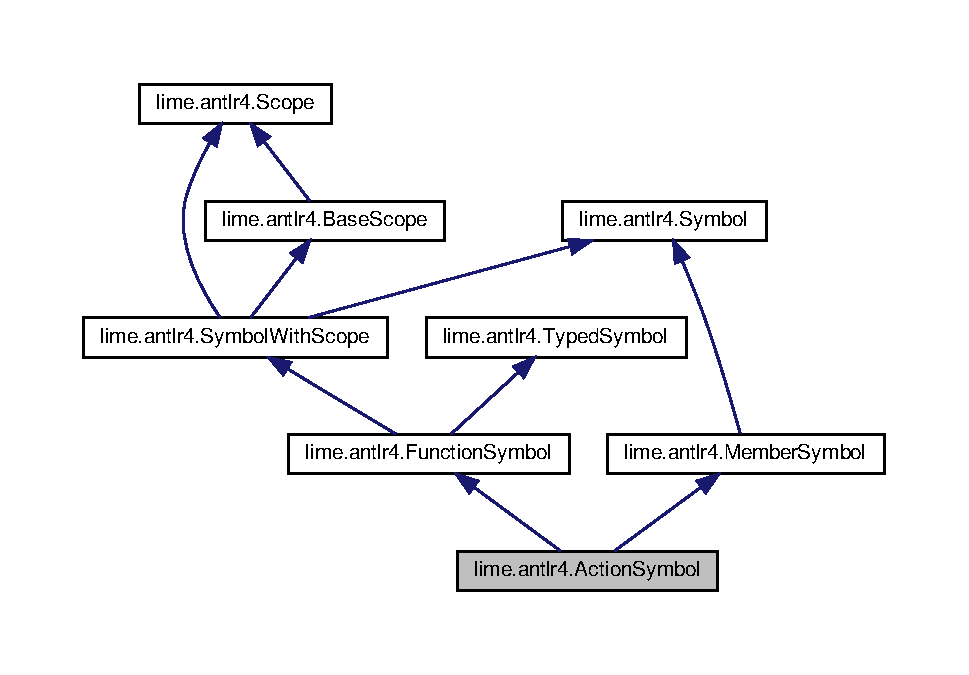
\includegraphics[width=350pt]{classlime_1_1antlr4_1_1ActionSymbol__inherit__graph}
\end{center}
\end{figure}


Collaboration diagram for lime.\+antlr4.\+Action\+Symbol\+:
\nopagebreak
\begin{figure}[H]
\begin{center}
\leavevmode
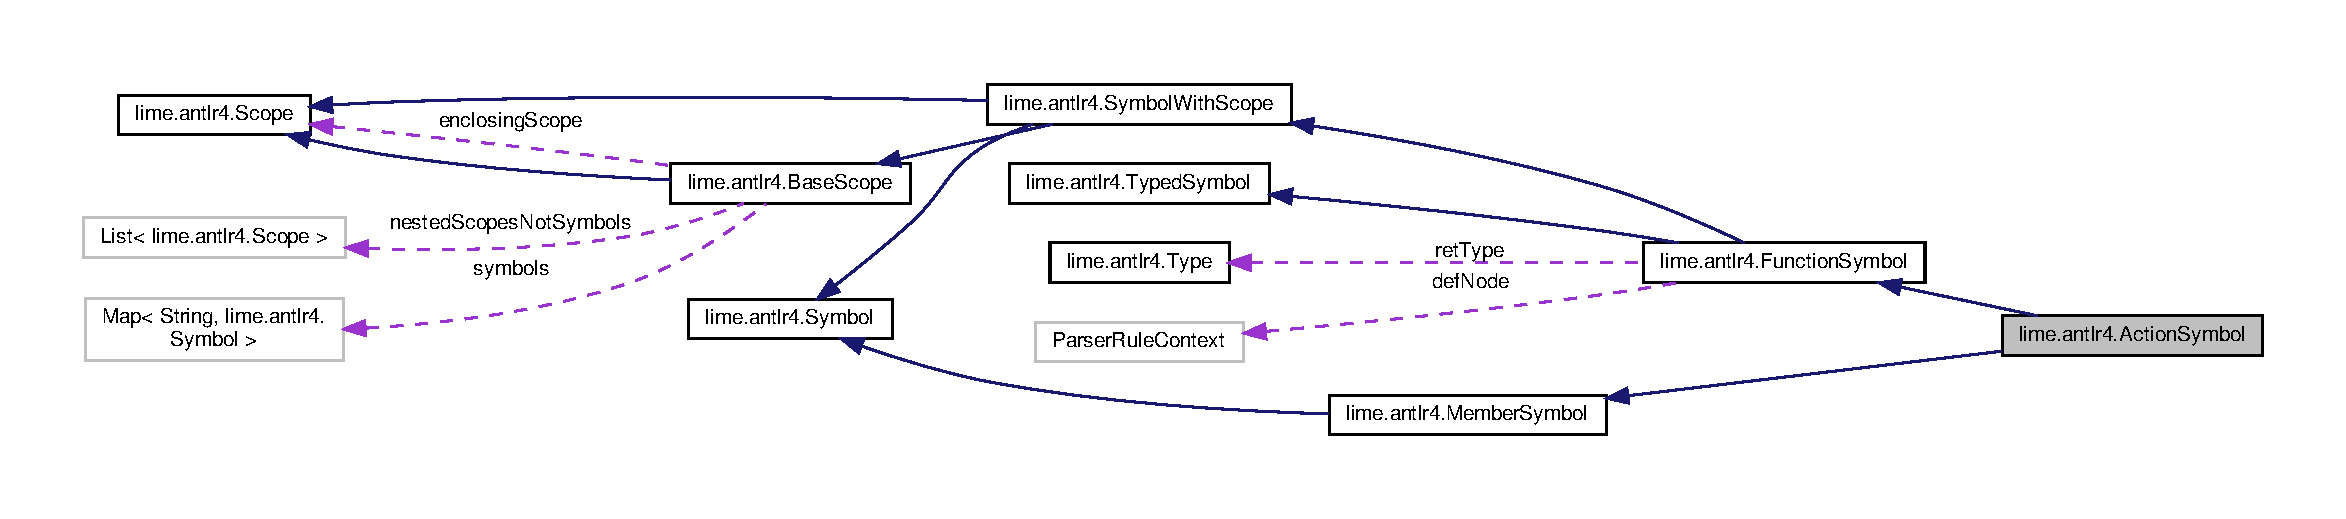
\includegraphics[width=350pt]{classlime_1_1antlr4_1_1ActionSymbol__coll__graph}
\end{center}
\end{figure}
\subsection*{Public Member Functions}
\begin{DoxyCompactItemize}
\item 
\mbox{\Hypertarget{classlime_1_1antlr4_1_1ActionSymbol_ad57bb5544fd2c738af25c16059d8ff0b}\label{classlime_1_1antlr4_1_1ActionSymbol_ad57bb5544fd2c738af25c16059d8ff0b}} 
{\bfseries Action\+Symbol} (String name)
\item 
\mbox{\Hypertarget{classlime_1_1antlr4_1_1ActionSymbol_a9a452118578a30c3cb31d9cade8cd81f}\label{classlime_1_1antlr4_1_1ActionSymbol_a9a452118578a30c3cb31d9cade8cd81f}} 
int {\bfseries get\+Slot\+Number} ()
\item 
\mbox{\Hypertarget{classlime_1_1antlr4_1_1ActionSymbol_a46ea3400662234b1382164bb38efacda}\label{classlime_1_1antlr4_1_1ActionSymbol_a46ea3400662234b1382164bb38efacda}} 
String {\bfseries to\+String} ()
\end{DoxyCompactItemize}
\subsection*{Static Protected Attributes}
\begin{DoxyCompactItemize}
\item 
\mbox{\Hypertarget{classlime_1_1antlr4_1_1ActionSymbol_a727c5b49c2845b1158796364ac0d923d}\label{classlime_1_1antlr4_1_1ActionSymbol_a727c5b49c2845b1158796364ac0d923d}} 
static int {\bfseries slot} = 0
\end{DoxyCompactItemize}
\subsection*{Additional Inherited Members}


The documentation for this class was generated from the following file\+:\begin{DoxyCompactItemize}
\item 
src/lime/antlr4/Action\+Symbol.\+java\end{DoxyCompactItemize}

\hypertarget{classlime_1_1antlr4_1_1ArrayType}{}\section{lime.\+antlr4.\+Array\+Type Class Reference}
\label{classlime_1_1antlr4_1_1ArrayType}\index{lime.\+antlr4.\+Array\+Type@{lime.\+antlr4.\+Array\+Type}}


Inheritance diagram for lime.\+antlr4.\+Array\+Type\+:
\nopagebreak
\begin{figure}[H]
\begin{center}
\leavevmode
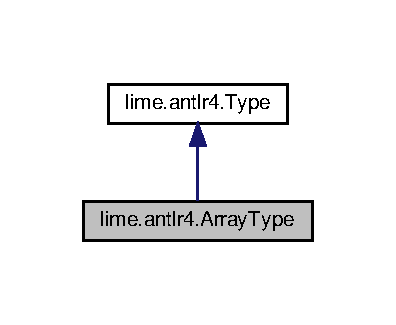
\includegraphics[width=190pt]{classlime_1_1antlr4_1_1ArrayType__inherit__graph}
\end{center}
\end{figure}


Collaboration diagram for lime.\+antlr4.\+Array\+Type\+:
\nopagebreak
\begin{figure}[H]
\begin{center}
\leavevmode
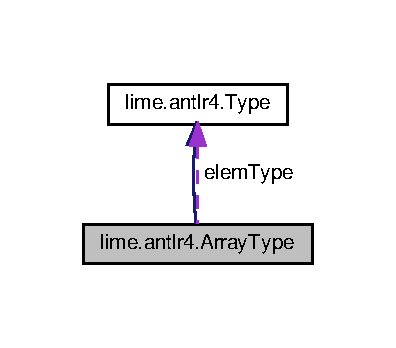
\includegraphics[width=190pt]{classlime_1_1antlr4_1_1ArrayType__coll__graph}
\end{center}
\end{figure}
\subsection*{Public Member Functions}
\begin{DoxyCompactItemize}
\item 
\mbox{\Hypertarget{classlime_1_1antlr4_1_1ArrayType_afe6a490ca32c9b6d5798fcfaf231c7ff}\label{classlime_1_1antlr4_1_1ArrayType_afe6a490ca32c9b6d5798fcfaf231c7ff}} 
{\bfseries Array\+Type} (\hyperlink{interfacelime_1_1antlr4_1_1Type}{Type} elem\+Type)
\item 
\mbox{\Hypertarget{classlime_1_1antlr4_1_1ArrayType_af36ad0edba10de016979212b51e2877d}\label{classlime_1_1antlr4_1_1ArrayType_af36ad0edba10de016979212b51e2877d}} 
{\bfseries Array\+Type} (\hyperlink{interfacelime_1_1antlr4_1_1Type}{Type} elem\+Type, int num\+Elems)
\item 
\mbox{\Hypertarget{classlime_1_1antlr4_1_1ArrayType_af14ca91720af7e3167b4eade114272ef}\label{classlime_1_1antlr4_1_1ArrayType_af14ca91720af7e3167b4eade114272ef}} 
String {\bfseries get\+Name} ()
\item 
\mbox{\Hypertarget{classlime_1_1antlr4_1_1ArrayType_ad5346eef4f4d200839de637a6abb5828}\label{classlime_1_1antlr4_1_1ArrayType_ad5346eef4f4d200839de637a6abb5828}} 
int {\bfseries get\+Type\+Index} ()
\item 
\mbox{\Hypertarget{classlime_1_1antlr4_1_1ArrayType_ad18c4bf92630ebfe65c3b37e22ef0010}\label{classlime_1_1antlr4_1_1ArrayType_ad18c4bf92630ebfe65c3b37e22ef0010}} 
String {\bfseries to\+String} ()
\end{DoxyCompactItemize}
\subsection*{Protected Attributes}
\begin{DoxyCompactItemize}
\item 
\mbox{\Hypertarget{classlime_1_1antlr4_1_1ArrayType_acdf1025cc8bdc8fd500a5033310b192b}\label{classlime_1_1antlr4_1_1ArrayType_acdf1025cc8bdc8fd500a5033310b192b}} 
final \hyperlink{interfacelime_1_1antlr4_1_1Type}{Type} {\bfseries elem\+Type}
\item 
\mbox{\Hypertarget{classlime_1_1antlr4_1_1ArrayType_afd97729bd1d371c2a008608298abfd5f}\label{classlime_1_1antlr4_1_1ArrayType_afd97729bd1d371c2a008608298abfd5f}} 
final int {\bfseries num\+Elems}
\end{DoxyCompactItemize}


The documentation for this class was generated from the following file\+:\begin{DoxyCompactItemize}
\item 
src/lime/antlr4/Array\+Type.\+java\end{DoxyCompactItemize}

\hypertarget{classlime_1_1antlr4_1_1BaseScope}{}\section{lime.\+antlr4.\+Base\+Scope Class Reference}
\label{classlime_1_1antlr4_1_1BaseScope}\index{lime.\+antlr4.\+Base\+Scope@{lime.\+antlr4.\+Base\+Scope}}


Inheritance diagram for lime.\+antlr4.\+Base\+Scope\+:
\nopagebreak
\begin{figure}[H]
\begin{center}
\leavevmode
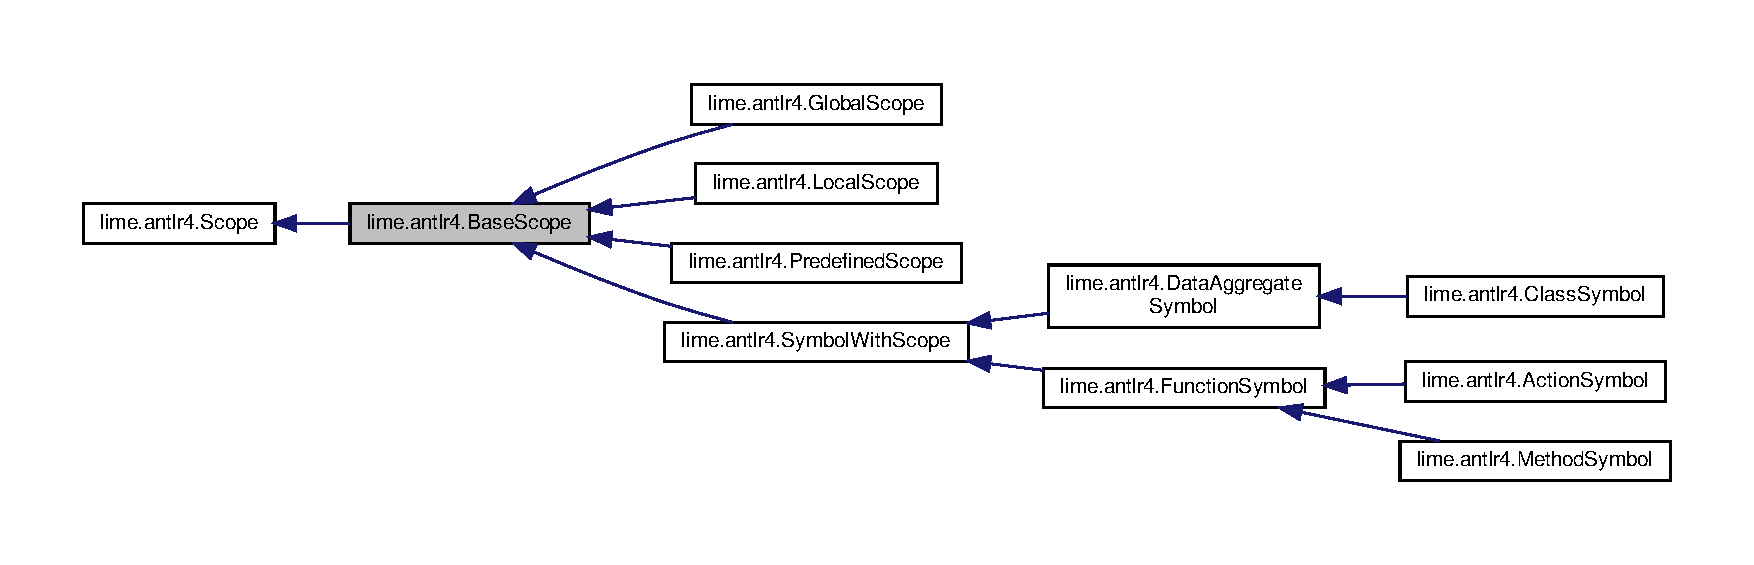
\includegraphics[width=350pt]{classlime_1_1antlr4_1_1BaseScope__inherit__graph}
\end{center}
\end{figure}


Collaboration diagram for lime.\+antlr4.\+Base\+Scope\+:
\nopagebreak
\begin{figure}[H]
\begin{center}
\leavevmode
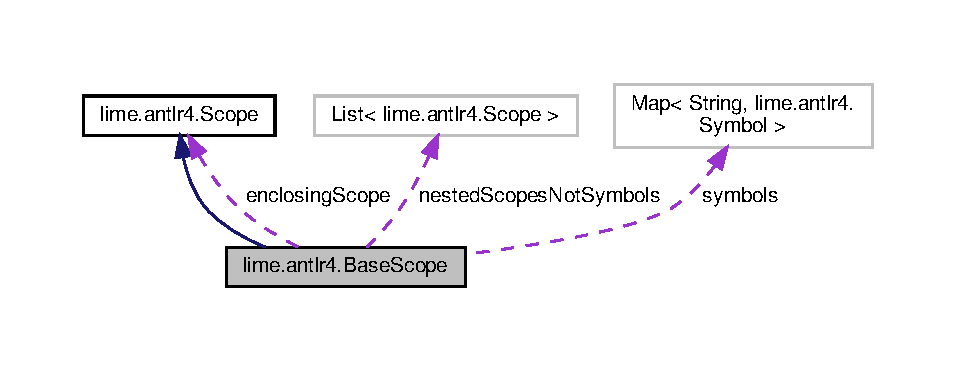
\includegraphics[width=350pt]{classlime_1_1antlr4_1_1BaseScope__coll__graph}
\end{center}
\end{figure}
\subsection*{Public Member Functions}
\begin{DoxyCompactItemize}
\item 
\mbox{\Hypertarget{classlime_1_1antlr4_1_1BaseScope_a8ca5b696eb960331183f728abe8086dd}\label{classlime_1_1antlr4_1_1BaseScope_a8ca5b696eb960331183f728abe8086dd}} 
{\bfseries Base\+Scope} (\hyperlink{interfacelime_1_1antlr4_1_1Scope}{Scope} enclosing\+Scope)
\item 
\mbox{\Hypertarget{classlime_1_1antlr4_1_1BaseScope_ae9182f1b315cc947b4eaf3ac538a6480}\label{classlime_1_1antlr4_1_1BaseScope_ae9182f1b315cc947b4eaf3ac538a6480}} 
Map$<$ String, ? extends \hyperlink{interfacelime_1_1antlr4_1_1Symbol}{Symbol} $>$ {\bfseries get\+Members} ()
\item 
\mbox{\Hypertarget{classlime_1_1antlr4_1_1BaseScope_a533c64421d34fe713263c587ebd7005b}\label{classlime_1_1antlr4_1_1BaseScope_a533c64421d34fe713263c587ebd7005b}} 
\hyperlink{interfacelime_1_1antlr4_1_1Symbol}{Symbol} {\bfseries get\+Symbol} (String name)
\item 
\mbox{\Hypertarget{classlime_1_1antlr4_1_1BaseScope_a5fbd1a473713f803eec4604d071cb317}\label{classlime_1_1antlr4_1_1BaseScope_a5fbd1a473713f803eec4604d071cb317}} 
void {\bfseries set\+Enclosing\+Scope} (\hyperlink{interfacelime_1_1antlr4_1_1Scope}{Scope} enclosing\+Scope)
\item 
\mbox{\Hypertarget{classlime_1_1antlr4_1_1BaseScope_acdbbd2fea0ca793aa75d506b99f1bdd8}\label{classlime_1_1antlr4_1_1BaseScope_acdbbd2fea0ca793aa75d506b99f1bdd8}} 
List$<$ \hyperlink{interfacelime_1_1antlr4_1_1Scope}{Scope} $>$ {\bfseries get\+All\+Nested\+Scoped\+Symbols} ()
\item 
\mbox{\Hypertarget{classlime_1_1antlr4_1_1BaseScope_a7bfdd5d3427f26887759f6e4ddc7497a}\label{classlime_1_1antlr4_1_1BaseScope_a7bfdd5d3427f26887759f6e4ddc7497a}} 
List$<$ \hyperlink{interfacelime_1_1antlr4_1_1Scope}{Scope} $>$ {\bfseries get\+Nested\+Scoped\+Symbols} ()
\item 
\mbox{\Hypertarget{classlime_1_1antlr4_1_1BaseScope_a6c3b48f4544d9bd317b3a276eef8b75d}\label{classlime_1_1antlr4_1_1BaseScope_a6c3b48f4544d9bd317b3a276eef8b75d}} 
List$<$ \hyperlink{interfacelime_1_1antlr4_1_1Scope}{Scope} $>$ {\bfseries get\+Nested\+Scopes} ()
\item 
void \hyperlink{classlime_1_1antlr4_1_1BaseScope_abef111b3380ebe06ea7ee7f160dae1d5}{nest} (\hyperlink{interfacelime_1_1antlr4_1_1Scope}{Scope} scope)  throws Illegal\+Argument\+Exception 
\item 
\mbox{\Hypertarget{classlime_1_1antlr4_1_1BaseScope_a02c825647d68c572b33fd3eae4f5aba4}\label{classlime_1_1antlr4_1_1BaseScope_a02c825647d68c572b33fd3eae4f5aba4}} 
\hyperlink{interfacelime_1_1antlr4_1_1Symbol}{Symbol} {\bfseries resolve} (String name)
\item 
\mbox{\Hypertarget{classlime_1_1antlr4_1_1BaseScope_a8c1c91f0ecf891905b1578ac026e453f}\label{classlime_1_1antlr4_1_1BaseScope_a8c1c91f0ecf891905b1578ac026e453f}} 
void {\bfseries define} (\hyperlink{interfacelime_1_1antlr4_1_1Symbol}{Symbol} sym)  throws Illegal\+Argument\+Exception 
\item 
\mbox{\Hypertarget{classlime_1_1antlr4_1_1BaseScope_a0ae6247a1ace7ef18fb30bd3cb10b2f1}\label{classlime_1_1antlr4_1_1BaseScope_a0ae6247a1ace7ef18fb30bd3cb10b2f1}} 
\hyperlink{interfacelime_1_1antlr4_1_1Scope}{Scope} {\bfseries get\+Enclosing\+Scope} ()
\item 
\hyperlink{interfacelime_1_1antlr4_1_1Scope}{Scope} \hyperlink{classlime_1_1antlr4_1_1BaseScope_affbef0d910750e3da48f581d10f68b68}{get\+Outer\+Most\+Enclosing\+Scope} ()
\item 
\hyperlink{classlime_1_1antlr4_1_1MethodSymbol}{Method\+Symbol} \hyperlink{classlime_1_1antlr4_1_1BaseScope_a3ec1571964f0556d2137fcaeacfe6ef2}{get\+Enclosing\+Scope\+Of\+Type} (Class$<$?$>$ type)
\item 
\mbox{\Hypertarget{classlime_1_1antlr4_1_1BaseScope_ad949a2376b037a965a06c5f12f3a0a8f}\label{classlime_1_1antlr4_1_1BaseScope_ad949a2376b037a965a06c5f12f3a0a8f}} 
List$<$ \hyperlink{interfacelime_1_1antlr4_1_1Scope}{Scope} $>$ {\bfseries get\+Enclosing\+Path\+To\+Root} ()
\item 
\mbox{\Hypertarget{classlime_1_1antlr4_1_1BaseScope_ad2e894a88f4b93ee6ea599953ee95954}\label{classlime_1_1antlr4_1_1BaseScope_ad2e894a88f4b93ee6ea599953ee95954}} 
List$<$? extends \hyperlink{interfacelime_1_1antlr4_1_1Symbol}{Symbol} $>$ {\bfseries get\+Symbols} ()
\item 
\mbox{\Hypertarget{classlime_1_1antlr4_1_1BaseScope_aef2ab699bb0b24e97d94435ee0b20de5}\label{classlime_1_1antlr4_1_1BaseScope_aef2ab699bb0b24e97d94435ee0b20de5}} 
List$<$? extends \hyperlink{interfacelime_1_1antlr4_1_1Symbol}{Symbol} $>$ {\bfseries get\+All\+Symbols} ()
\item 
\mbox{\Hypertarget{classlime_1_1antlr4_1_1BaseScope_a9c2788f3e688f3c3c33eb5044919c4a5}\label{classlime_1_1antlr4_1_1BaseScope_a9c2788f3e688f3c3c33eb5044919c4a5}} 
\hyperlink{interfacelime_1_1antlr4_1_1Symbol}{Symbol} {\bfseries find\+Symbol} (String name)
\item 
\mbox{\Hypertarget{classlime_1_1antlr4_1_1BaseScope_afbe0ff3e90cbba8ad2e9486f71e1a38b}\label{classlime_1_1antlr4_1_1BaseScope_afbe0ff3e90cbba8ad2e9486f71e1a38b}} 
int {\bfseries get\+Number\+Of\+Symbols} ()
\item 
\mbox{\Hypertarget{classlime_1_1antlr4_1_1BaseScope_a2df91cc9ada5859c7827f3fcfad32153}\label{classlime_1_1antlr4_1_1BaseScope_a2df91cc9ada5859c7827f3fcfad32153}} 
Set$<$ String $>$ {\bfseries get\+Symbol\+Names} ()
\item 
\mbox{\Hypertarget{classlime_1_1antlr4_1_1BaseScope_a58c2ca0ff03936e91d080ed2b0213f42}\label{classlime_1_1antlr4_1_1BaseScope_a58c2ca0ff03936e91d080ed2b0213f42}} 
String {\bfseries to\+String} ()
\item 
\mbox{\Hypertarget{classlime_1_1antlr4_1_1BaseScope_a6cb0d6a6a322a651becba56ce2082425}\label{classlime_1_1antlr4_1_1BaseScope_a6cb0d6a6a322a651becba56ce2082425}} 
String {\bfseries to\+Scope\+Stack\+String} (String separator)
\item 
\mbox{\Hypertarget{classlime_1_1antlr4_1_1BaseScope_a7cba137da26469b1ec56c29a74ba749f}\label{classlime_1_1antlr4_1_1BaseScope_a7cba137da26469b1ec56c29a74ba749f}} 
String {\bfseries to\+Qualifier\+String} (String separator)
\item 
\mbox{\Hypertarget{classlime_1_1antlr4_1_1BaseScope_ae8278e6d3457895e73bd180334ced59f}\label{classlime_1_1antlr4_1_1BaseScope_ae8278e6d3457895e73bd180334ced59f}} 
String {\bfseries to\+Test\+String} ()
\item 
\mbox{\Hypertarget{classlime_1_1antlr4_1_1BaseScope_ac9c771b481325b78aab6a06630314c0e}\label{classlime_1_1antlr4_1_1BaseScope_ac9c771b481325b78aab6a06630314c0e}} 
String {\bfseries to\+Test\+String} (String separator, String scope\+Path\+Separator)
\end{DoxyCompactItemize}
\subsection*{Protected Attributes}
\begin{DoxyCompactItemize}
\item 
\mbox{\Hypertarget{classlime_1_1antlr4_1_1BaseScope_a03d117a3d5c9d40796ffdf3e74f7866f}\label{classlime_1_1antlr4_1_1BaseScope_a03d117a3d5c9d40796ffdf3e74f7866f}} 
\hyperlink{interfacelime_1_1antlr4_1_1Scope}{Scope} {\bfseries enclosing\+Scope}
\item 
\mbox{\Hypertarget{classlime_1_1antlr4_1_1BaseScope_ade889728bb27b5aa13f772f5ab18bdc4}\label{classlime_1_1antlr4_1_1BaseScope_ade889728bb27b5aa13f772f5ab18bdc4}} 
Map$<$ String, \hyperlink{interfacelime_1_1antlr4_1_1Symbol}{Symbol} $>$ {\bfseries symbols} = new Linked\+Hash\+Map$<$$>$()
\item 
\mbox{\Hypertarget{classlime_1_1antlr4_1_1BaseScope_afe902a8fa79fe6e6efe74b9209d6bfef}\label{classlime_1_1antlr4_1_1BaseScope_afe902a8fa79fe6e6efe74b9209d6bfef}} 
List$<$ \hyperlink{interfacelime_1_1antlr4_1_1Scope}{Scope} $>$ {\bfseries nested\+Scopes\+Not\+Symbols} = new Array\+List$<$$>$()
\end{DoxyCompactItemize}


\subsection{Member Function Documentation}
\mbox{\Hypertarget{classlime_1_1antlr4_1_1BaseScope_a3ec1571964f0556d2137fcaeacfe6ef2}\label{classlime_1_1antlr4_1_1BaseScope_a3ec1571964f0556d2137fcaeacfe6ef2}} 
\index{lime\+::antlr4\+::\+Base\+Scope@{lime\+::antlr4\+::\+Base\+Scope}!get\+Enclosing\+Scope\+Of\+Type@{get\+Enclosing\+Scope\+Of\+Type}}
\index{get\+Enclosing\+Scope\+Of\+Type@{get\+Enclosing\+Scope\+Of\+Type}!lime\+::antlr4\+::\+Base\+Scope@{lime\+::antlr4\+::\+Base\+Scope}}
\subsubsection{\texorpdfstring{get\+Enclosing\+Scope\+Of\+Type()}{getEnclosingScopeOfType()}}
{\footnotesize\ttfamily \hyperlink{classlime_1_1antlr4_1_1MethodSymbol}{Method\+Symbol} lime.\+antlr4.\+Base\+Scope.\+get\+Enclosing\+Scope\+Of\+Type (\begin{DoxyParamCaption}\item[{Class$<$?$>$}]{type }\end{DoxyParamCaption})}

Walk up enclosing\+Scope until we find an object of a specific type. E.\+g., if you want to get enclosing method, you would pass in Method\+Symbol.\+class, unless of course you have created a subclass for your language implementation. Here is the call graph for this function\+:
\nopagebreak
\begin{figure}[H]
\begin{center}
\leavevmode
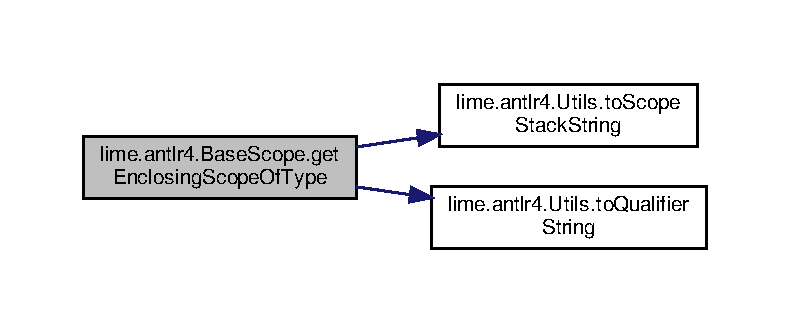
\includegraphics[width=350pt]{classlime_1_1antlr4_1_1BaseScope_a3ec1571964f0556d2137fcaeacfe6ef2_cgraph}
\end{center}
\end{figure}
\mbox{\Hypertarget{classlime_1_1antlr4_1_1BaseScope_affbef0d910750e3da48f581d10f68b68}\label{classlime_1_1antlr4_1_1BaseScope_affbef0d910750e3da48f581d10f68b68}} 
\index{lime\+::antlr4\+::\+Base\+Scope@{lime\+::antlr4\+::\+Base\+Scope}!get\+Outer\+Most\+Enclosing\+Scope@{get\+Outer\+Most\+Enclosing\+Scope}}
\index{get\+Outer\+Most\+Enclosing\+Scope@{get\+Outer\+Most\+Enclosing\+Scope}!lime\+::antlr4\+::\+Base\+Scope@{lime\+::antlr4\+::\+Base\+Scope}}
\subsubsection{\texorpdfstring{get\+Outer\+Most\+Enclosing\+Scope()}{getOuterMostEnclosingScope()}}
{\footnotesize\ttfamily \hyperlink{interfacelime_1_1antlr4_1_1Scope}{Scope} lime.\+antlr4.\+Base\+Scope.\+get\+Outer\+Most\+Enclosing\+Scope (\begin{DoxyParamCaption}{ }\end{DoxyParamCaption})}

Walk up enclosing\+Scope until we find topmost. Note this is enclosing scope not necessarily parent. This will usually be a global scope or something, depending on your scope tree. \mbox{\Hypertarget{classlime_1_1antlr4_1_1BaseScope_abef111b3380ebe06ea7ee7f160dae1d5}\label{classlime_1_1antlr4_1_1BaseScope_abef111b3380ebe06ea7ee7f160dae1d5}} 
\index{lime\+::antlr4\+::\+Base\+Scope@{lime\+::antlr4\+::\+Base\+Scope}!nest@{nest}}
\index{nest@{nest}!lime\+::antlr4\+::\+Base\+Scope@{lime\+::antlr4\+::\+Base\+Scope}}
\subsubsection{\texorpdfstring{nest()}{nest()}}
{\footnotesize\ttfamily void lime.\+antlr4.\+Base\+Scope.\+nest (\begin{DoxyParamCaption}\item[{\hyperlink{interfacelime_1_1antlr4_1_1Scope}{Scope}}]{scope }\end{DoxyParamCaption}) throws Illegal\+Argument\+Exception}

Add a nested scope to this scope; could also be a \hyperlink{classlime_1_1antlr4_1_1FunctionSymbol}{Function\+Symbol} if your language allows nested functions. 

Implements \hyperlink{interfacelime_1_1antlr4_1_1Scope}{lime.\+antlr4.\+Scope}.



The documentation for this class was generated from the following file\+:\begin{DoxyCompactItemize}
\item 
src/lime/antlr4/Base\+Scope.\+java\end{DoxyCompactItemize}

\hypertarget{classlime_1_1antlr4_1_1BaseSymbol}{}\section{lime.\+antlr4.\+Base\+Symbol Class Reference}
\label{classlime_1_1antlr4_1_1BaseSymbol}\index{lime.\+antlr4.\+Base\+Symbol@{lime.\+antlr4.\+Base\+Symbol}}


Inheritance diagram for lime.\+antlr4.\+Base\+Symbol\+:
\nopagebreak
\begin{figure}[H]
\begin{center}
\leavevmode
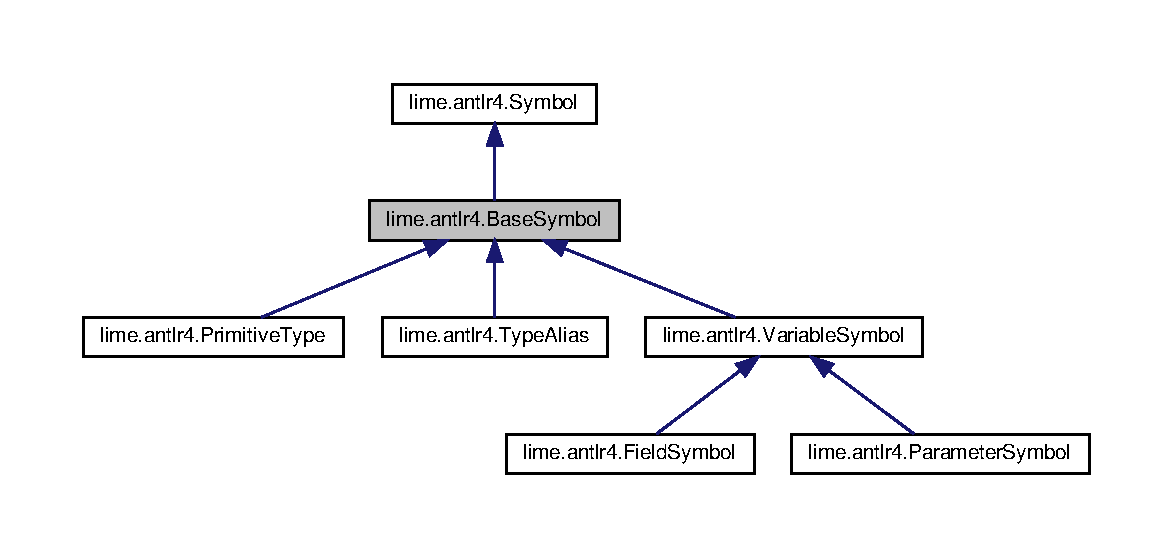
\includegraphics[width=350pt]{classlime_1_1antlr4_1_1BaseSymbol__inherit__graph}
\end{center}
\end{figure}


Collaboration diagram for lime.\+antlr4.\+Base\+Symbol\+:
\nopagebreak
\begin{figure}[H]
\begin{center}
\leavevmode
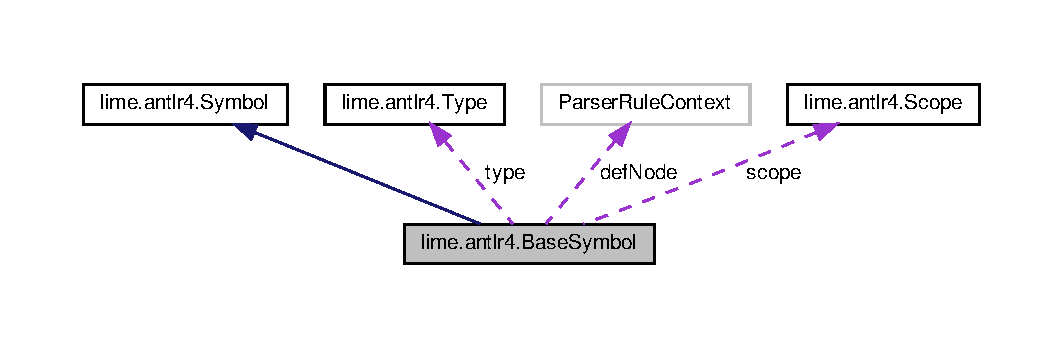
\includegraphics[width=350pt]{classlime_1_1antlr4_1_1BaseSymbol__coll__graph}
\end{center}
\end{figure}
\subsection*{Public Member Functions}
\begin{DoxyCompactItemize}
\item 
\mbox{\Hypertarget{classlime_1_1antlr4_1_1BaseSymbol_ac575dfc1fadf1efd8c7197017355bf7e}\label{classlime_1_1antlr4_1_1BaseSymbol_ac575dfc1fadf1efd8c7197017355bf7e}} 
{\bfseries Base\+Symbol} (String name)
\item 
\mbox{\Hypertarget{classlime_1_1antlr4_1_1BaseSymbol_a6cd9f668fd2553d3444dec00f078fce8}\label{classlime_1_1antlr4_1_1BaseSymbol_a6cd9f668fd2553d3444dec00f078fce8}} 
String {\bfseries get\+Name} ()
\item 
\mbox{\Hypertarget{classlime_1_1antlr4_1_1BaseSymbol_a754f241ca15fe70367daf886ee4f4758}\label{classlime_1_1antlr4_1_1BaseSymbol_a754f241ca15fe70367daf886ee4f4758}} 
\hyperlink{interfacelime_1_1antlr4_1_1Scope}{Scope} {\bfseries get\+Scope} ()
\item 
\mbox{\Hypertarget{classlime_1_1antlr4_1_1BaseSymbol_a89120a47e263a491a108be43f9a9d212}\label{classlime_1_1antlr4_1_1BaseSymbol_a89120a47e263a491a108be43f9a9d212}} 
void {\bfseries set\+Scope} (\hyperlink{interfacelime_1_1antlr4_1_1Scope}{Scope} scope)
\item 
\mbox{\Hypertarget{classlime_1_1antlr4_1_1BaseSymbol_a5129b86389fda744a1c6607240a18e64}\label{classlime_1_1antlr4_1_1BaseSymbol_a5129b86389fda744a1c6607240a18e64}} 
\hyperlink{interfacelime_1_1antlr4_1_1Type}{Type} {\bfseries get\+Type} ()
\item 
\mbox{\Hypertarget{classlime_1_1antlr4_1_1BaseSymbol_a8cd6f5d691c221a5fea181ff956a2d5a}\label{classlime_1_1antlr4_1_1BaseSymbol_a8cd6f5d691c221a5fea181ff956a2d5a}} 
void {\bfseries set\+Type} (\hyperlink{interfacelime_1_1antlr4_1_1Type}{Type} type)
\item 
\mbox{\Hypertarget{classlime_1_1antlr4_1_1BaseSymbol_a6136bb5d8b7fd373b75f809bf216660c}\label{classlime_1_1antlr4_1_1BaseSymbol_a6136bb5d8b7fd373b75f809bf216660c}} 
void {\bfseries set\+Def\+Node} (Parser\+Rule\+Context def\+Node)
\item 
\mbox{\Hypertarget{classlime_1_1antlr4_1_1BaseSymbol_affe1bffdbf0663559e15130b1388fad4}\label{classlime_1_1antlr4_1_1BaseSymbol_affe1bffdbf0663559e15130b1388fad4}} 
Parser\+Rule\+Context {\bfseries get\+Def\+Node} ()
\item 
\mbox{\Hypertarget{classlime_1_1antlr4_1_1BaseSymbol_a3d8c2602c8d04f5d9d1d47b2d8e92c20}\label{classlime_1_1antlr4_1_1BaseSymbol_a3d8c2602c8d04f5d9d1d47b2d8e92c20}} 
boolean {\bfseries equals} (Object obj)
\item 
\mbox{\Hypertarget{classlime_1_1antlr4_1_1BaseSymbol_a751b0abe7249c5fe0d3b1d6d7df8fe42}\label{classlime_1_1antlr4_1_1BaseSymbol_a751b0abe7249c5fe0d3b1d6d7df8fe42}} 
int {\bfseries hash\+Code} ()
\item 
\mbox{\Hypertarget{classlime_1_1antlr4_1_1BaseSymbol_aa6fe99025a62bc81423dbc06d979ca94}\label{classlime_1_1antlr4_1_1BaseSymbol_aa6fe99025a62bc81423dbc06d979ca94}} 
int {\bfseries get\+Insertion\+Order\+Number} ()
\item 
\mbox{\Hypertarget{classlime_1_1antlr4_1_1BaseSymbol_a58a350b374bb0f0de7babdd90ab9bd84}\label{classlime_1_1antlr4_1_1BaseSymbol_a58a350b374bb0f0de7babdd90ab9bd84}} 
void {\bfseries set\+Insertion\+Order\+Number} (int i)
\item 
\mbox{\Hypertarget{classlime_1_1antlr4_1_1BaseSymbol_a994af1cc58ec3d293c8c4af4465889ad}\label{classlime_1_1antlr4_1_1BaseSymbol_a994af1cc58ec3d293c8c4af4465889ad}} 
String {\bfseries get\+Fully\+Qualified\+Name} (String scope\+Path\+Separator)
\item 
\mbox{\Hypertarget{classlime_1_1antlr4_1_1BaseSymbol_a04a7f7972a61c30e9ea4cf02350286b4}\label{classlime_1_1antlr4_1_1BaseSymbol_a04a7f7972a61c30e9ea4cf02350286b4}} 
String {\bfseries to\+String} ()
\end{DoxyCompactItemize}
\subsection*{Protected Attributes}
\begin{DoxyCompactItemize}
\item 
\mbox{\Hypertarget{classlime_1_1antlr4_1_1BaseSymbol_ab56d427263f9becd162f7f2c5ee6bac8}\label{classlime_1_1antlr4_1_1BaseSymbol_ab56d427263f9becd162f7f2c5ee6bac8}} 
final String {\bfseries name}
\item 
\mbox{\Hypertarget{classlime_1_1antlr4_1_1BaseSymbol_a950da5974a979aff4431e27a067fc67a}\label{classlime_1_1antlr4_1_1BaseSymbol_a950da5974a979aff4431e27a067fc67a}} 
\hyperlink{interfacelime_1_1antlr4_1_1Type}{Type} {\bfseries type}
\item 
\mbox{\Hypertarget{classlime_1_1antlr4_1_1BaseSymbol_a2466b0e9d5abfffcdcfd85872175af9a}\label{classlime_1_1antlr4_1_1BaseSymbol_a2466b0e9d5abfffcdcfd85872175af9a}} 
\hyperlink{interfacelime_1_1antlr4_1_1Scope}{Scope} {\bfseries scope}
\item 
\mbox{\Hypertarget{classlime_1_1antlr4_1_1BaseSymbol_a29643bf09e99211b2c7c622426c90fdf}\label{classlime_1_1antlr4_1_1BaseSymbol_a29643bf09e99211b2c7c622426c90fdf}} 
Parser\+Rule\+Context {\bfseries def\+Node}
\item 
\mbox{\Hypertarget{classlime_1_1antlr4_1_1BaseSymbol_aa96ed257b534e0652e37cb2cb7b510ac}\label{classlime_1_1antlr4_1_1BaseSymbol_aa96ed257b534e0652e37cb2cb7b510ac}} 
int {\bfseries lexical\+Order}
\end{DoxyCompactItemize}


The documentation for this class was generated from the following file\+:\begin{DoxyCompactItemize}
\item 
src/lime/antlr4/Base\+Symbol.\+java\end{DoxyCompactItemize}

\hypertarget{classlime_1_1antlr4_1_1Builder}{}\section{lime.\+antlr4.\+Builder Class Reference}
\label{classlime_1_1antlr4_1_1Builder}\index{lime.\+antlr4.\+Builder@{lime.\+antlr4.\+Builder}}
\subsection*{Classes}
\begin{DoxyCompactItemize}
\item 
class {\bfseries Lexer}
\item 
class {\bfseries Parser}
\item 
class {\bfseries Tree}
\end{DoxyCompactItemize}


The documentation for this class was generated from the following file\+:\begin{DoxyCompactItemize}
\item 
src/lime/antlr4/Builder.\+java\end{DoxyCompactItemize}

\hypertarget{classlime_1_1antlr4_1_1ClassSymbol}{}\section{lime.\+antlr4.\+Class\+Symbol Class Reference}
\label{classlime_1_1antlr4_1_1ClassSymbol}\index{lime.\+antlr4.\+Class\+Symbol@{lime.\+antlr4.\+Class\+Symbol}}


Inheritance diagram for lime.\+antlr4.\+Class\+Symbol\+:
\nopagebreak
\begin{figure}[H]
\begin{center}
\leavevmode
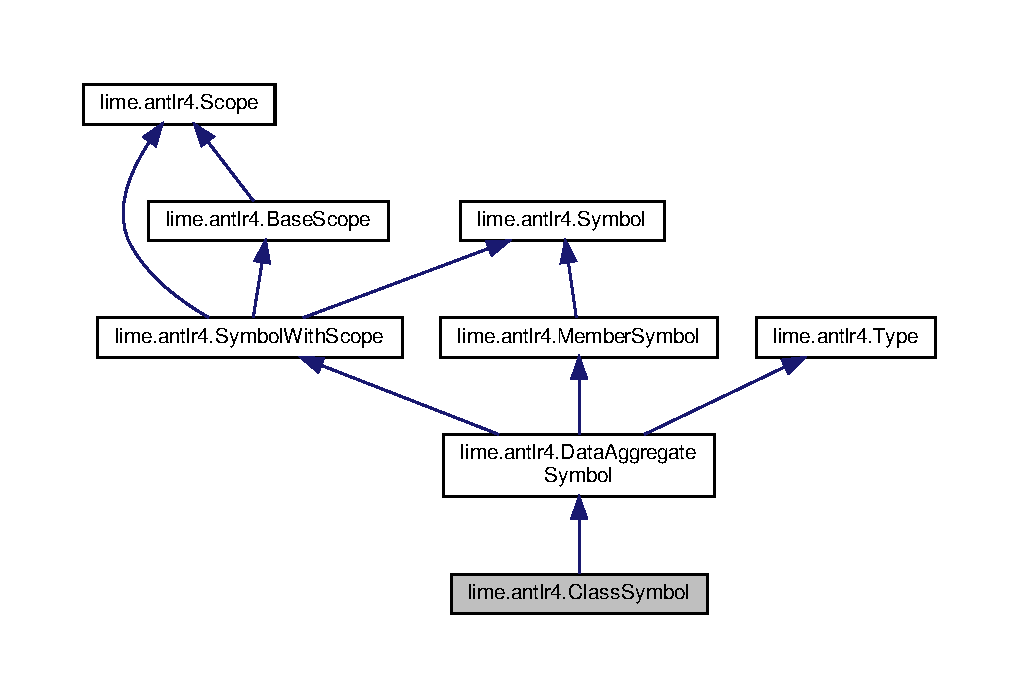
\includegraphics[width=350pt]{classlime_1_1antlr4_1_1ClassSymbol__inherit__graph}
\end{center}
\end{figure}


Collaboration diagram for lime.\+antlr4.\+Class\+Symbol\+:
\nopagebreak
\begin{figure}[H]
\begin{center}
\leavevmode
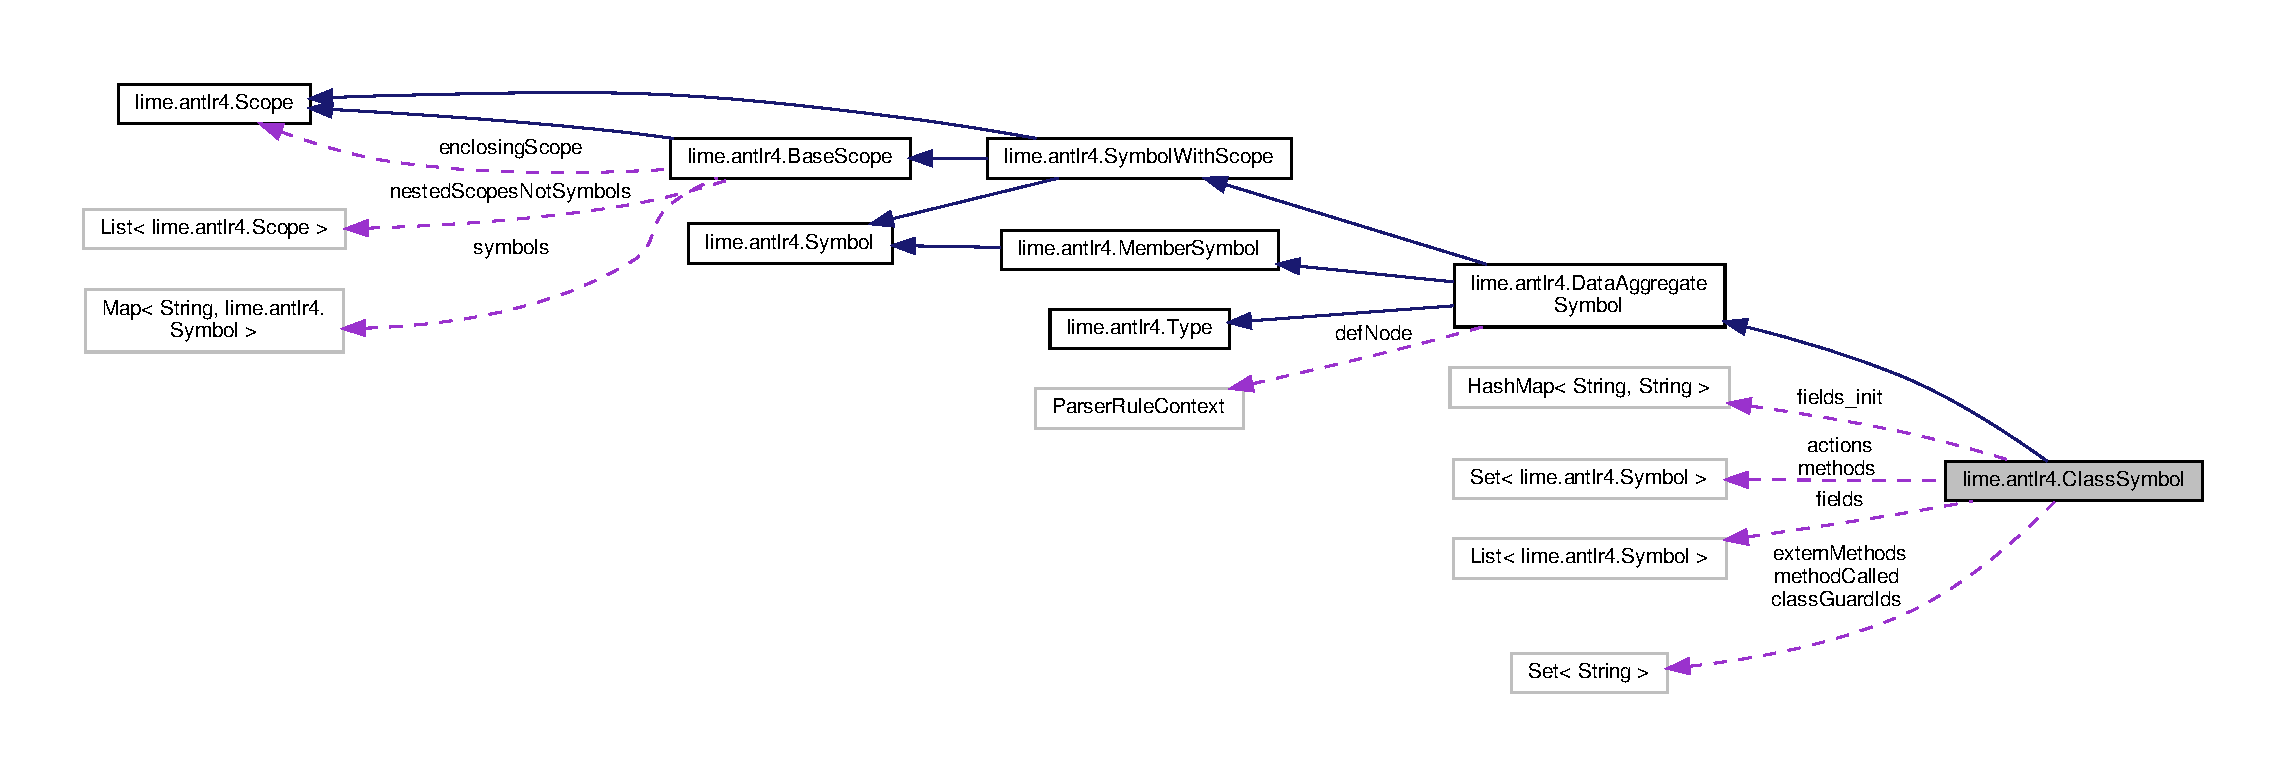
\includegraphics[width=350pt]{classlime_1_1antlr4_1_1ClassSymbol__coll__graph}
\end{center}
\end{figure}
\subsection*{Public Member Functions}
\begin{DoxyCompactItemize}
\item 
\mbox{\Hypertarget{classlime_1_1antlr4_1_1ClassSymbol_a2aca5ee207d7ea16740b505a0e9409f6}\label{classlime_1_1antlr4_1_1ClassSymbol_a2aca5ee207d7ea16740b505a0e9409f6}} 
{\bfseries Class\+Symbol} (String name)
\item 
\mbox{\Hypertarget{classlime_1_1antlr4_1_1ClassSymbol_ab9deb43e9c146c98c8f988f8eda8ab4a}\label{classlime_1_1antlr4_1_1ClassSymbol_ab9deb43e9c146c98c8f988f8eda8ab4a}} 
void {\bfseries add\+External\+Function} ()
\item 
\mbox{\Hypertarget{classlime_1_1antlr4_1_1ClassSymbol_a50068ed8eba46e8e4d59305b69649f52}\label{classlime_1_1antlr4_1_1ClassSymbol_a50068ed8eba46e8e4d59305b69649f52}} 
void {\bfseries set\+Obj\+Init\+Code} (String in)
\item 
\mbox{\Hypertarget{classlime_1_1antlr4_1_1ClassSymbol_a79ea5e2f896c15184664d53f2b96c0c4}\label{classlime_1_1antlr4_1_1ClassSymbol_a79ea5e2f896c15184664d53f2b96c0c4}} 
String {\bfseries get\+Obj\+Init\+Code} ()
\item 
\hyperlink{classlime_1_1antlr4_1_1ClassSymbol}{Class\+Symbol} \hyperlink{classlime_1_1antlr4_1_1ClassSymbol_a9f660dd54d7ab8643fb885669adad106}{get\+Super\+Class\+Scope} ()
\item 
List$<$ \hyperlink{classlime_1_1antlr4_1_1ClassSymbol}{Class\+Symbol} $>$ \hyperlink{classlime_1_1antlr4_1_1ClassSymbol_a6505cf7d9bbc2b32620eab9e20ddb881}{get\+Super\+Class\+Scopes} ()
\item 
\mbox{\Hypertarget{classlime_1_1antlr4_1_1ClassSymbol_ae4de50f9edf4a6aff80835352e9a8039}\label{classlime_1_1antlr4_1_1ClassSymbol_ae4de50f9edf4a6aff80835352e9a8039}} 
\hyperlink{interfacelime_1_1antlr4_1_1Symbol}{Symbol} {\bfseries resolve} (String name)
\item 
\hyperlink{interfacelime_1_1antlr4_1_1Symbol}{Symbol} \hyperlink{classlime_1_1antlr4_1_1ClassSymbol_a6bf9bcc8721faa0f5c61b9134e8ddf37}{resolve\+Member} (String name)
\item 
\hyperlink{interfacelime_1_1antlr4_1_1Symbol}{Symbol} \hyperlink{classlime_1_1antlr4_1_1ClassSymbol_a3b5e6abcf9e0c8be368f0aa77f58db1e}{resolve\+Field} (String name)
\item 
\hyperlink{classlime_1_1antlr4_1_1MethodSymbol}{Method\+Symbol} \hyperlink{classlime_1_1antlr4_1_1ClassSymbol_a8b22f82d150b8c2fce1330ce7e570bb9}{resolve\+Method} (String name)
\item 
\hyperlink{classlime_1_1antlr4_1_1ActionSymbol}{Action\+Symbol} \hyperlink{classlime_1_1antlr4_1_1ClassSymbol_a5f03ec543ef043695007844d15614b2c}{resolve\+Action} (String name)
\item 
\mbox{\Hypertarget{classlime_1_1antlr4_1_1ClassSymbol_a7a572167b09bb6e79fa4df1560bafb2b}\label{classlime_1_1antlr4_1_1ClassSymbol_a7a572167b09bb6e79fa4df1560bafb2b}} 
void {\bfseries set\+Super\+Class} (String super\+Class\+Name)
\item 
\mbox{\Hypertarget{classlime_1_1antlr4_1_1ClassSymbol_af6106c3a7c1701e59c88ff87a7ecdb64}\label{classlime_1_1antlr4_1_1ClassSymbol_af6106c3a7c1701e59c88ff87a7ecdb64}} 
String {\bfseries get\+Super\+Class\+Name} ()
\item 
\mbox{\Hypertarget{classlime_1_1antlr4_1_1ClassSymbol_a524d88d04bb503fab001ce85cdf3b47f}\label{classlime_1_1antlr4_1_1ClassSymbol_a524d88d04bb503fab001ce85cdf3b47f}} 
void {\bfseries set\+Slot\+Number} (\hyperlink{interfacelime_1_1antlr4_1_1Symbol}{Symbol} sym)
\item 
Set$<$ \hyperlink{classlime_1_1antlr4_1_1MethodSymbol}{Method\+Symbol} $>$ \hyperlink{classlime_1_1antlr4_1_1ClassSymbol_aefa7b605f712bc843830b4e66d547962}{get\+Defined\+Methods} ()
\item 
Set$<$ \hyperlink{classlime_1_1antlr4_1_1MethodSymbol}{Method\+Symbol} $>$ \hyperlink{classlime_1_1antlr4_1_1ClassSymbol_a0bb56898dfcbdc91a1f81151524b54f5}{get\+Methods} ()
\item 
Set$<$ \hyperlink{classlime_1_1antlr4_1_1ActionSymbol}{Action\+Symbol} $>$ \hyperlink{classlime_1_1antlr4_1_1ClassSymbol_a44bf9a31b2d4f8f92ae7314ccb7fac8a}{get\+Defined\+Actions} ()
\item 
Set$<$ \hyperlink{classlime_1_1antlr4_1_1ActionSymbol}{Action\+Symbol} $>$ \hyperlink{classlime_1_1antlr4_1_1ClassSymbol_a18650f607ed0d77dda29df41cfd0f1cc}{get\+Actions} ()
\item 
\mbox{\Hypertarget{classlime_1_1antlr4_1_1ClassSymbol_a00d51f3e82f50c3a2c0bcaf03db5f29e}\label{classlime_1_1antlr4_1_1ClassSymbol_a00d51f3e82f50c3a2c0bcaf03db5f29e}} 
List$<$? extends \hyperlink{classlime_1_1antlr4_1_1FieldSymbol}{Field\+Symbol} $>$ {\bfseries get\+Fields} ()
\item 
\mbox{\Hypertarget{classlime_1_1antlr4_1_1ClassSymbol_a96bdb39c0c64f2ecb26aeee3057f8ec3}\label{classlime_1_1antlr4_1_1ClassSymbol_a96bdb39c0c64f2ecb26aeee3057f8ec3}} 
int {\bfseries get\+Field\+Index} (String s)
\item 
int \hyperlink{classlime_1_1antlr4_1_1ClassSymbol_a885f4e871c5b078980c39db6385506cb}{get\+Number\+Of\+Defined\+Methods} ()
\item 
int \hyperlink{classlime_1_1antlr4_1_1ClassSymbol_a2cbf5115ef39f615447ea46a777cbb9f}{get\+Number\+Of\+Defined\+Actions} ()
\item 
int \hyperlink{classlime_1_1antlr4_1_1ClassSymbol_a3f6bef449ae63455b81793f897a0c7e9}{get\+Number\+Of\+Methods} ()
\item 
int \hyperlink{classlime_1_1antlr4_1_1ClassSymbol_a2d505f3b8d3fe0727ff72b55195a3b6e}{get\+Number\+Of\+Actions} ()
\item 
\mbox{\Hypertarget{classlime_1_1antlr4_1_1ClassSymbol_ae60eda30124bbcefd3adb0c694c7f3c4}\label{classlime_1_1antlr4_1_1ClassSymbol_ae60eda30124bbcefd3adb0c694c7f3c4}} 
int {\bfseries get\+Number\+Of\+Fields} ()
\item 
\mbox{\Hypertarget{classlime_1_1antlr4_1_1ClassSymbol_adc9fde793561674436cfd7c13ce61e93}\label{classlime_1_1antlr4_1_1ClassSymbol_adc9fde793561674436cfd7c13ce61e93}} 
String {\bfseries to\+String} ()
\end{DoxyCompactItemize}
\subsection*{Public Attributes}
\begin{DoxyCompactItemize}
\item 
\mbox{\Hypertarget{classlime_1_1antlr4_1_1ClassSymbol_a9f999815c2d73172a6cf39537646dc44}\label{classlime_1_1antlr4_1_1ClassSymbol_a9f999815c2d73172a6cf39537646dc44}} 
Set$<$ String $>$ {\bfseries method\+Called}
\item 
\mbox{\Hypertarget{classlime_1_1antlr4_1_1ClassSymbol_a680722e0d3e297093b3f731986491cf9}\label{classlime_1_1antlr4_1_1ClassSymbol_a680722e0d3e297093b3f731986491cf9}} 
Set$<$ String $>$ {\bfseries class\+Guard\+Ids}
\item 
\mbox{\Hypertarget{classlime_1_1antlr4_1_1ClassSymbol_a705d66c00e52c5987258a7c5bc913e2d}\label{classlime_1_1antlr4_1_1ClassSymbol_a705d66c00e52c5987258a7c5bc913e2d}} 
Set$<$ String $>$ {\bfseries extern\+Methods}
\end{DoxyCompactItemize}
\subsection*{Protected Attributes}
\begin{DoxyCompactItemize}
\item 
\mbox{\Hypertarget{classlime_1_1antlr4_1_1ClassSymbol_a614bdac77f637b1a26d4dd77adec48de}\label{classlime_1_1antlr4_1_1ClassSymbol_a614bdac77f637b1a26d4dd77adec48de}} 
String {\bfseries super\+Class\+Name}
\item 
\mbox{\Hypertarget{classlime_1_1antlr4_1_1ClassSymbol_a43628f8649fc6107ccb5dba1045e3f39}\label{classlime_1_1antlr4_1_1ClassSymbol_a43628f8649fc6107ccb5dba1045e3f39}} 
int {\bfseries next\+Free\+Method\+Slot} = 0
\item 
\mbox{\Hypertarget{classlime_1_1antlr4_1_1ClassSymbol_a1612136c011a497c79963acedc55308c}\label{classlime_1_1antlr4_1_1ClassSymbol_a1612136c011a497c79963acedc55308c}} 
int {\bfseries next\+Free\+Action\+Slot} = 0
\end{DoxyCompactItemize}


\subsection{Detailed Description}
A symbol representing the class. It is a kind of data aggregate that has much in common with a struct. 

\subsection{Member Function Documentation}
\mbox{\Hypertarget{classlime_1_1antlr4_1_1ClassSymbol_a18650f607ed0d77dda29df41cfd0f1cc}\label{classlime_1_1antlr4_1_1ClassSymbol_a18650f607ed0d77dda29df41cfd0f1cc}} 
\index{lime\+::antlr4\+::\+Class\+Symbol@{lime\+::antlr4\+::\+Class\+Symbol}!get\+Actions@{get\+Actions}}
\index{get\+Actions@{get\+Actions}!lime\+::antlr4\+::\+Class\+Symbol@{lime\+::antlr4\+::\+Class\+Symbol}}
\subsubsection{\texorpdfstring{get\+Actions()}{getActions()}}
{\footnotesize\ttfamily Set$<$\hyperlink{classlime_1_1antlr4_1_1ActionSymbol}{Action\+Symbol}$>$ lime.\+antlr4.\+Class\+Symbol.\+get\+Actions (\begin{DoxyParamCaption}{ }\end{DoxyParamCaption})}

Return the set of all actions either inherited or not Here is the call graph for this function\+:
\nopagebreak
\begin{figure}[H]
\begin{center}
\leavevmode
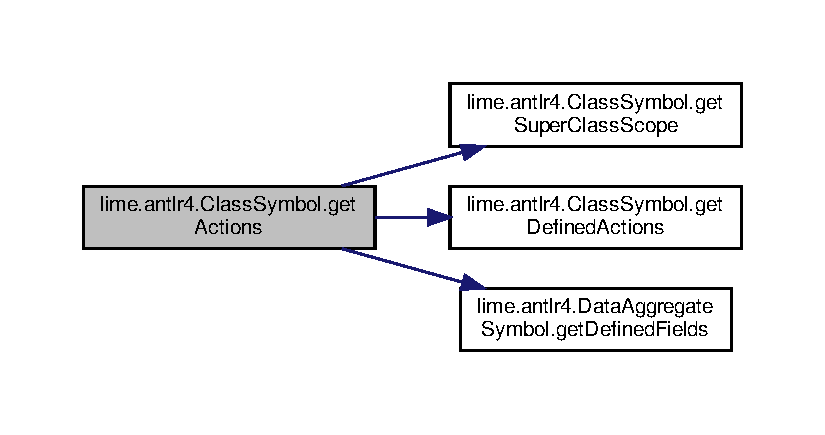
\includegraphics[width=350pt]{classlime_1_1antlr4_1_1ClassSymbol_a18650f607ed0d77dda29df41cfd0f1cc_cgraph}
\end{center}
\end{figure}
\mbox{\Hypertarget{classlime_1_1antlr4_1_1ClassSymbol_a44bf9a31b2d4f8f92ae7314ccb7fac8a}\label{classlime_1_1antlr4_1_1ClassSymbol_a44bf9a31b2d4f8f92ae7314ccb7fac8a}} 
\index{lime\+::antlr4\+::\+Class\+Symbol@{lime\+::antlr4\+::\+Class\+Symbol}!get\+Defined\+Actions@{get\+Defined\+Actions}}
\index{get\+Defined\+Actions@{get\+Defined\+Actions}!lime\+::antlr4\+::\+Class\+Symbol@{lime\+::antlr4\+::\+Class\+Symbol}}
\subsubsection{\texorpdfstring{get\+Defined\+Actions()}{getDefinedActions()}}
{\footnotesize\ttfamily Set$<$\hyperlink{classlime_1_1antlr4_1_1ActionSymbol}{Action\+Symbol}$>$ lime.\+antlr4.\+Class\+Symbol.\+get\+Defined\+Actions (\begin{DoxyParamCaption}{ }\end{DoxyParamCaption})}

Return the set of all actions defined within this class \mbox{\Hypertarget{classlime_1_1antlr4_1_1ClassSymbol_aefa7b605f712bc843830b4e66d547962}\label{classlime_1_1antlr4_1_1ClassSymbol_aefa7b605f712bc843830b4e66d547962}} 
\index{lime\+::antlr4\+::\+Class\+Symbol@{lime\+::antlr4\+::\+Class\+Symbol}!get\+Defined\+Methods@{get\+Defined\+Methods}}
\index{get\+Defined\+Methods@{get\+Defined\+Methods}!lime\+::antlr4\+::\+Class\+Symbol@{lime\+::antlr4\+::\+Class\+Symbol}}
\subsubsection{\texorpdfstring{get\+Defined\+Methods()}{getDefinedMethods()}}
{\footnotesize\ttfamily Set$<$\hyperlink{classlime_1_1antlr4_1_1MethodSymbol}{Method\+Symbol}$>$ lime.\+antlr4.\+Class\+Symbol.\+get\+Defined\+Methods (\begin{DoxyParamCaption}{ }\end{DoxyParamCaption})}

Return the set of all methods defined within this class \mbox{\Hypertarget{classlime_1_1antlr4_1_1ClassSymbol_a0bb56898dfcbdc91a1f81151524b54f5}\label{classlime_1_1antlr4_1_1ClassSymbol_a0bb56898dfcbdc91a1f81151524b54f5}} 
\index{lime\+::antlr4\+::\+Class\+Symbol@{lime\+::antlr4\+::\+Class\+Symbol}!get\+Methods@{get\+Methods}}
\index{get\+Methods@{get\+Methods}!lime\+::antlr4\+::\+Class\+Symbol@{lime\+::antlr4\+::\+Class\+Symbol}}
\subsubsection{\texorpdfstring{get\+Methods()}{getMethods()}}
{\footnotesize\ttfamily Set$<$\hyperlink{classlime_1_1antlr4_1_1MethodSymbol}{Method\+Symbol}$>$ lime.\+antlr4.\+Class\+Symbol.\+get\+Methods (\begin{DoxyParamCaption}{ }\end{DoxyParamCaption})}

Return the set of all methods either inherited or not Here is the call graph for this function\+:
\nopagebreak
\begin{figure}[H]
\begin{center}
\leavevmode
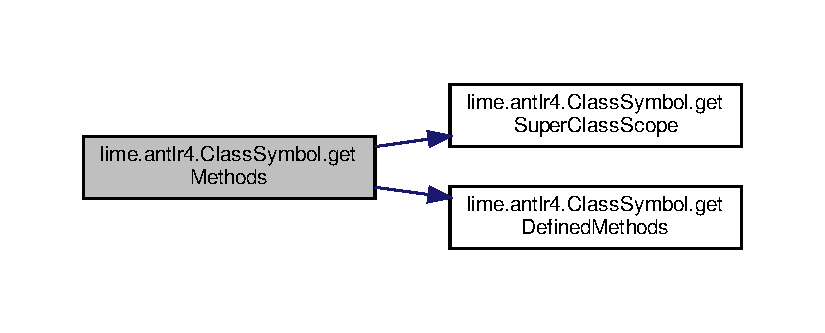
\includegraphics[width=350pt]{classlime_1_1antlr4_1_1ClassSymbol_a0bb56898dfcbdc91a1f81151524b54f5_cgraph}
\end{center}
\end{figure}
\mbox{\Hypertarget{classlime_1_1antlr4_1_1ClassSymbol_a2d505f3b8d3fe0727ff72b55195a3b6e}\label{classlime_1_1antlr4_1_1ClassSymbol_a2d505f3b8d3fe0727ff72b55195a3b6e}} 
\index{lime\+::antlr4\+::\+Class\+Symbol@{lime\+::antlr4\+::\+Class\+Symbol}!get\+Number\+Of\+Actions@{get\+Number\+Of\+Actions}}
\index{get\+Number\+Of\+Actions@{get\+Number\+Of\+Actions}!lime\+::antlr4\+::\+Class\+Symbol@{lime\+::antlr4\+::\+Class\+Symbol}}
\subsubsection{\texorpdfstring{get\+Number\+Of\+Actions()}{getNumberOfActions()}}
{\footnotesize\ttfamily int lime.\+antlr4.\+Class\+Symbol.\+get\+Number\+Of\+Actions (\begin{DoxyParamCaption}{ }\end{DoxyParamCaption})}

get the total number of actions visible to this class Here is the call graph for this function\+:
\nopagebreak
\begin{figure}[H]
\begin{center}
\leavevmode
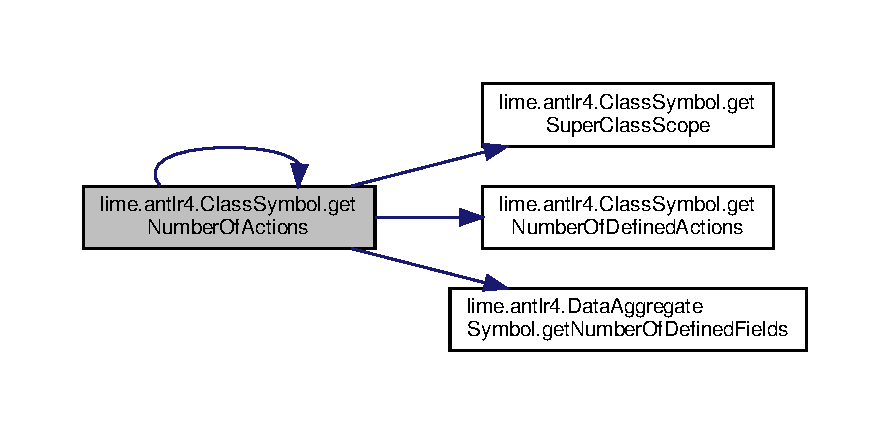
\includegraphics[width=350pt]{classlime_1_1antlr4_1_1ClassSymbol_a2d505f3b8d3fe0727ff72b55195a3b6e_cgraph}
\end{center}
\end{figure}
\mbox{\Hypertarget{classlime_1_1antlr4_1_1ClassSymbol_a2cbf5115ef39f615447ea46a777cbb9f}\label{classlime_1_1antlr4_1_1ClassSymbol_a2cbf5115ef39f615447ea46a777cbb9f}} 
\index{lime\+::antlr4\+::\+Class\+Symbol@{lime\+::antlr4\+::\+Class\+Symbol}!get\+Number\+Of\+Defined\+Actions@{get\+Number\+Of\+Defined\+Actions}}
\index{get\+Number\+Of\+Defined\+Actions@{get\+Number\+Of\+Defined\+Actions}!lime\+::antlr4\+::\+Class\+Symbol@{lime\+::antlr4\+::\+Class\+Symbol}}
\subsubsection{\texorpdfstring{get\+Number\+Of\+Defined\+Actions()}{getNumberOfDefinedActions()}}
{\footnotesize\ttfamily int lime.\+antlr4.\+Class\+Symbol.\+get\+Number\+Of\+Defined\+Actions (\begin{DoxyParamCaption}{ }\end{DoxyParamCaption})}

get the number of actions defined specifically in this class \mbox{\Hypertarget{classlime_1_1antlr4_1_1ClassSymbol_a885f4e871c5b078980c39db6385506cb}\label{classlime_1_1antlr4_1_1ClassSymbol_a885f4e871c5b078980c39db6385506cb}} 
\index{lime\+::antlr4\+::\+Class\+Symbol@{lime\+::antlr4\+::\+Class\+Symbol}!get\+Number\+Of\+Defined\+Methods@{get\+Number\+Of\+Defined\+Methods}}
\index{get\+Number\+Of\+Defined\+Methods@{get\+Number\+Of\+Defined\+Methods}!lime\+::antlr4\+::\+Class\+Symbol@{lime\+::antlr4\+::\+Class\+Symbol}}
\subsubsection{\texorpdfstring{get\+Number\+Of\+Defined\+Methods()}{getNumberOfDefinedMethods()}}
{\footnotesize\ttfamily int lime.\+antlr4.\+Class\+Symbol.\+get\+Number\+Of\+Defined\+Methods (\begin{DoxyParamCaption}{ }\end{DoxyParamCaption})}

get the number of methods defined specifically in this class \mbox{\Hypertarget{classlime_1_1antlr4_1_1ClassSymbol_a3f6bef449ae63455b81793f897a0c7e9}\label{classlime_1_1antlr4_1_1ClassSymbol_a3f6bef449ae63455b81793f897a0c7e9}} 
\index{lime\+::antlr4\+::\+Class\+Symbol@{lime\+::antlr4\+::\+Class\+Symbol}!get\+Number\+Of\+Methods@{get\+Number\+Of\+Methods}}
\index{get\+Number\+Of\+Methods@{get\+Number\+Of\+Methods}!lime\+::antlr4\+::\+Class\+Symbol@{lime\+::antlr4\+::\+Class\+Symbol}}
\subsubsection{\texorpdfstring{get\+Number\+Of\+Methods()}{getNumberOfMethods()}}
{\footnotesize\ttfamily int lime.\+antlr4.\+Class\+Symbol.\+get\+Number\+Of\+Methods (\begin{DoxyParamCaption}{ }\end{DoxyParamCaption})}

get the total number of methods visible to this class Here is the call graph for this function\+:
\nopagebreak
\begin{figure}[H]
\begin{center}
\leavevmode
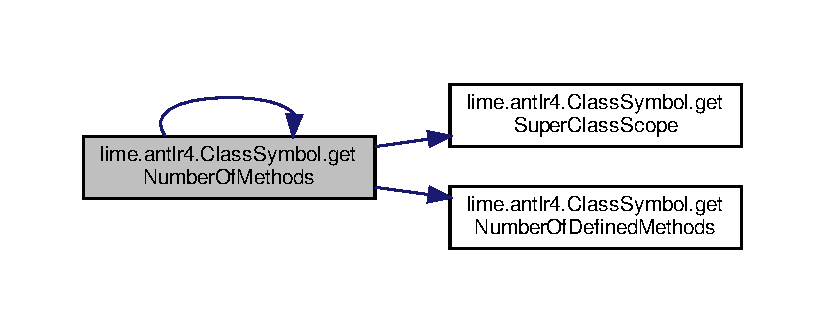
\includegraphics[width=350pt]{classlime_1_1antlr4_1_1ClassSymbol_a3f6bef449ae63455b81793f897a0c7e9_cgraph}
\end{center}
\end{figure}
\mbox{\Hypertarget{classlime_1_1antlr4_1_1ClassSymbol_a9f660dd54d7ab8643fb885669adad106}\label{classlime_1_1antlr4_1_1ClassSymbol_a9f660dd54d7ab8643fb885669adad106}} 
\index{lime\+::antlr4\+::\+Class\+Symbol@{lime\+::antlr4\+::\+Class\+Symbol}!get\+Super\+Class\+Scope@{get\+Super\+Class\+Scope}}
\index{get\+Super\+Class\+Scope@{get\+Super\+Class\+Scope}!lime\+::antlr4\+::\+Class\+Symbol@{lime\+::antlr4\+::\+Class\+Symbol}}
\subsubsection{\texorpdfstring{get\+Super\+Class\+Scope()}{getSuperClassScope()}}
{\footnotesize\ttfamily \hyperlink{classlime_1_1antlr4_1_1ClassSymbol}{Class\+Symbol} lime.\+antlr4.\+Class\+Symbol.\+get\+Super\+Class\+Scope (\begin{DoxyParamCaption}{ }\end{DoxyParamCaption})}

Return the \hyperlink{classlime_1_1antlr4_1_1ClassSymbol}{Class\+Symbol} associated with super\+Class\+Name or null if superclass is not resolved looking up the enclosing scope chain. \mbox{\Hypertarget{classlime_1_1antlr4_1_1ClassSymbol_a6505cf7d9bbc2b32620eab9e20ddb881}\label{classlime_1_1antlr4_1_1ClassSymbol_a6505cf7d9bbc2b32620eab9e20ddb881}} 
\index{lime\+::antlr4\+::\+Class\+Symbol@{lime\+::antlr4\+::\+Class\+Symbol}!get\+Super\+Class\+Scopes@{get\+Super\+Class\+Scopes}}
\index{get\+Super\+Class\+Scopes@{get\+Super\+Class\+Scopes}!lime\+::antlr4\+::\+Class\+Symbol@{lime\+::antlr4\+::\+Class\+Symbol}}
\subsubsection{\texorpdfstring{get\+Super\+Class\+Scopes()}{getSuperClassScopes()}}
{\footnotesize\ttfamily List$<$\hyperlink{classlime_1_1antlr4_1_1ClassSymbol}{Class\+Symbol}$>$ lime.\+antlr4.\+Class\+Symbol.\+get\+Super\+Class\+Scopes (\begin{DoxyParamCaption}{ }\end{DoxyParamCaption})}

Multiple superclass or interface implementations and the like... Here is the call graph for this function\+:
\nopagebreak
\begin{figure}[H]
\begin{center}
\leavevmode
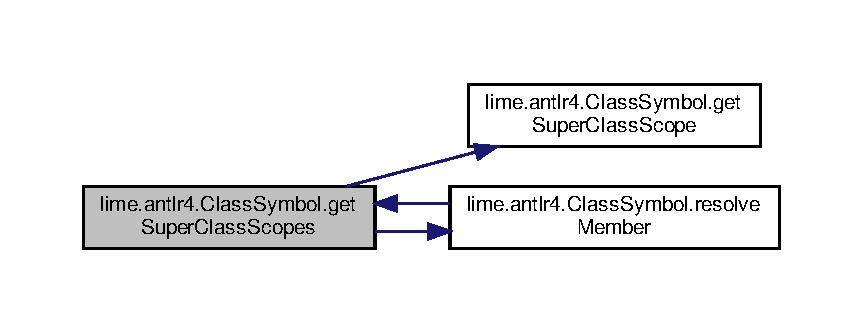
\includegraphics[width=350pt]{classlime_1_1antlr4_1_1ClassSymbol_a6505cf7d9bbc2b32620eab9e20ddb881_cgraph}
\end{center}
\end{figure}
\mbox{\Hypertarget{classlime_1_1antlr4_1_1ClassSymbol_a5f03ec543ef043695007844d15614b2c}\label{classlime_1_1antlr4_1_1ClassSymbol_a5f03ec543ef043695007844d15614b2c}} 
\index{lime\+::antlr4\+::\+Class\+Symbol@{lime\+::antlr4\+::\+Class\+Symbol}!resolve\+Action@{resolve\+Action}}
\index{resolve\+Action@{resolve\+Action}!lime\+::antlr4\+::\+Class\+Symbol@{lime\+::antlr4\+::\+Class\+Symbol}}
\subsubsection{\texorpdfstring{resolve\+Action()}{resolveAction()}}
{\footnotesize\ttfamily \hyperlink{classlime_1_1antlr4_1_1ActionSymbol}{Action\+Symbol} lime.\+antlr4.\+Class\+Symbol.\+resolve\+Action (\begin{DoxyParamCaption}\item[{String}]{name }\end{DoxyParamCaption})}

Look for a action with this name in this scope or any super class. Return null if no method found. Here is the call graph for this function\+:
\nopagebreak
\begin{figure}[H]
\begin{center}
\leavevmode
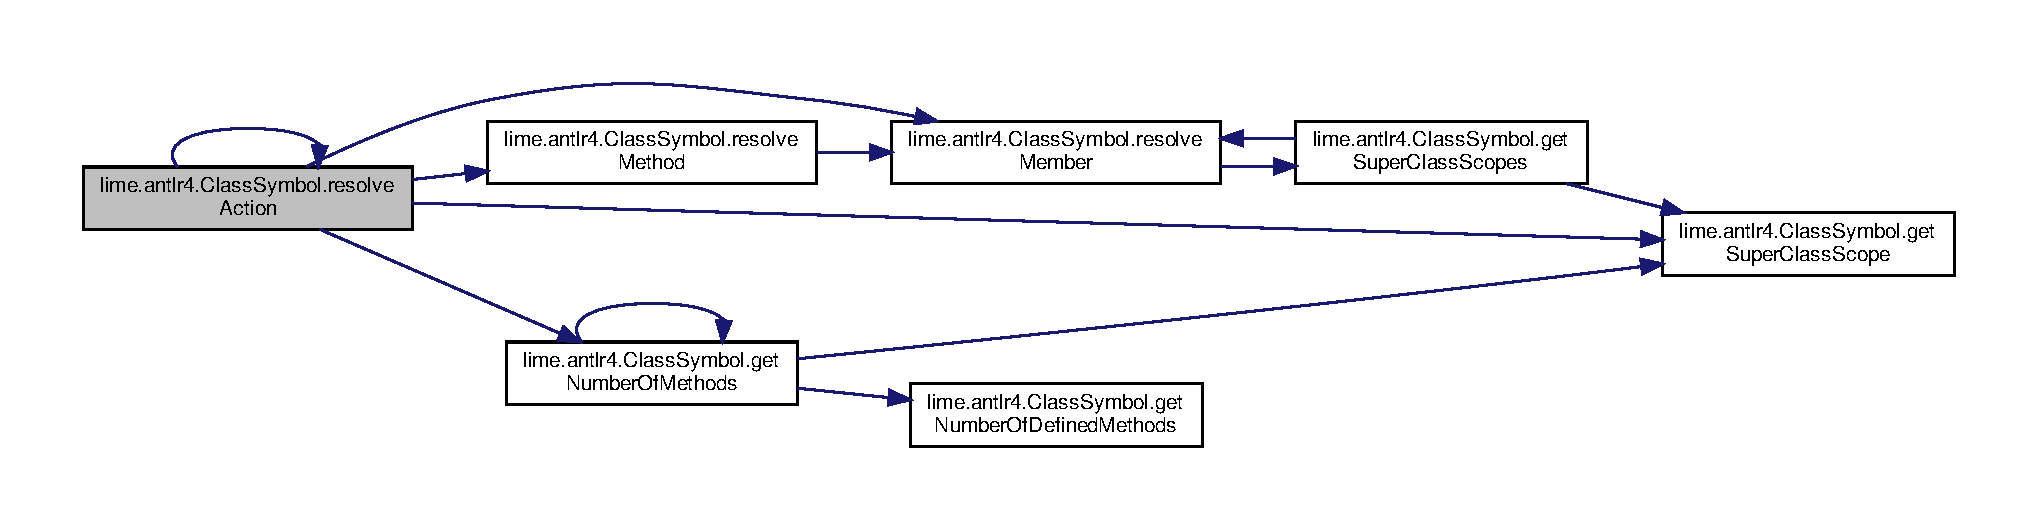
\includegraphics[width=350pt]{classlime_1_1antlr4_1_1ClassSymbol_a5f03ec543ef043695007844d15614b2c_cgraph}
\end{center}
\end{figure}
\mbox{\Hypertarget{classlime_1_1antlr4_1_1ClassSymbol_a3b5e6abcf9e0c8be368f0aa77f58db1e}\label{classlime_1_1antlr4_1_1ClassSymbol_a3b5e6abcf9e0c8be368f0aa77f58db1e}} 
\index{lime\+::antlr4\+::\+Class\+Symbol@{lime\+::antlr4\+::\+Class\+Symbol}!resolve\+Field@{resolve\+Field}}
\index{resolve\+Field@{resolve\+Field}!lime\+::antlr4\+::\+Class\+Symbol@{lime\+::antlr4\+::\+Class\+Symbol}}
\subsubsection{\texorpdfstring{resolve\+Field()}{resolveField()}}
{\footnotesize\ttfamily \hyperlink{interfacelime_1_1antlr4_1_1Symbol}{Symbol} lime.\+antlr4.\+Class\+Symbol.\+resolve\+Field (\begin{DoxyParamCaption}\item[{String}]{name }\end{DoxyParamCaption})}

Look for a field with this name in this scope or any super class. Return null if no field found. Here is the call graph for this function\+:
\nopagebreak
\begin{figure}[H]
\begin{center}
\leavevmode
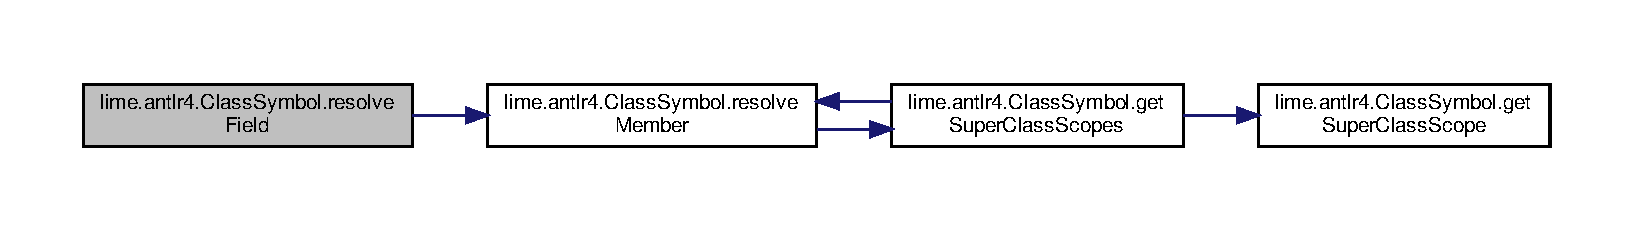
\includegraphics[width=350pt]{classlime_1_1antlr4_1_1ClassSymbol_a3b5e6abcf9e0c8be368f0aa77f58db1e_cgraph}
\end{center}
\end{figure}
\mbox{\Hypertarget{classlime_1_1antlr4_1_1ClassSymbol_a6bf9bcc8721faa0f5c61b9134e8ddf37}\label{classlime_1_1antlr4_1_1ClassSymbol_a6bf9bcc8721faa0f5c61b9134e8ddf37}} 
\index{lime\+::antlr4\+::\+Class\+Symbol@{lime\+::antlr4\+::\+Class\+Symbol}!resolve\+Member@{resolve\+Member}}
\index{resolve\+Member@{resolve\+Member}!lime\+::antlr4\+::\+Class\+Symbol@{lime\+::antlr4\+::\+Class\+Symbol}}
\subsubsection{\texorpdfstring{resolve\+Member()}{resolveMember()}}
{\footnotesize\ttfamily \hyperlink{interfacelime_1_1antlr4_1_1Symbol}{Symbol} lime.\+antlr4.\+Class\+Symbol.\+resolve\+Member (\begin{DoxyParamCaption}\item[{String}]{name }\end{DoxyParamCaption})}

Look for a member with this name in this scope or any super class. Return null if no member found. Here is the call graph for this function\+:
\nopagebreak
\begin{figure}[H]
\begin{center}
\leavevmode
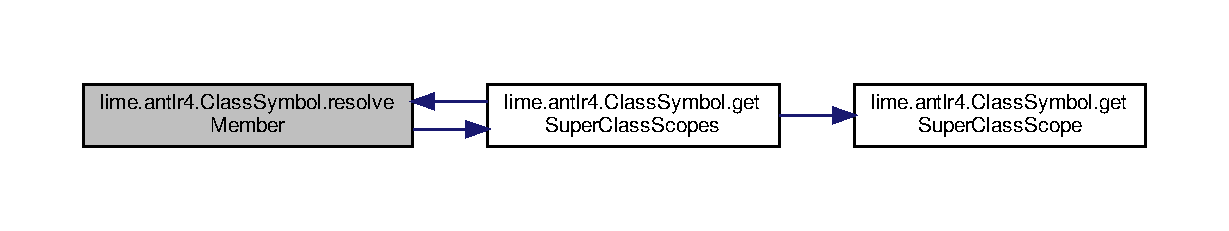
\includegraphics[width=350pt]{classlime_1_1antlr4_1_1ClassSymbol_a6bf9bcc8721faa0f5c61b9134e8ddf37_cgraph}
\end{center}
\end{figure}
\mbox{\Hypertarget{classlime_1_1antlr4_1_1ClassSymbol_a8b22f82d150b8c2fce1330ce7e570bb9}\label{classlime_1_1antlr4_1_1ClassSymbol_a8b22f82d150b8c2fce1330ce7e570bb9}} 
\index{lime\+::antlr4\+::\+Class\+Symbol@{lime\+::antlr4\+::\+Class\+Symbol}!resolve\+Method@{resolve\+Method}}
\index{resolve\+Method@{resolve\+Method}!lime\+::antlr4\+::\+Class\+Symbol@{lime\+::antlr4\+::\+Class\+Symbol}}
\subsubsection{\texorpdfstring{resolve\+Method()}{resolveMethod()}}
{\footnotesize\ttfamily \hyperlink{classlime_1_1antlr4_1_1MethodSymbol}{Method\+Symbol} lime.\+antlr4.\+Class\+Symbol.\+resolve\+Method (\begin{DoxyParamCaption}\item[{String}]{name }\end{DoxyParamCaption})}

Look for a method with this name in this scope or any super class. Return null if no method found. Here is the call graph for this function\+:
\nopagebreak
\begin{figure}[H]
\begin{center}
\leavevmode
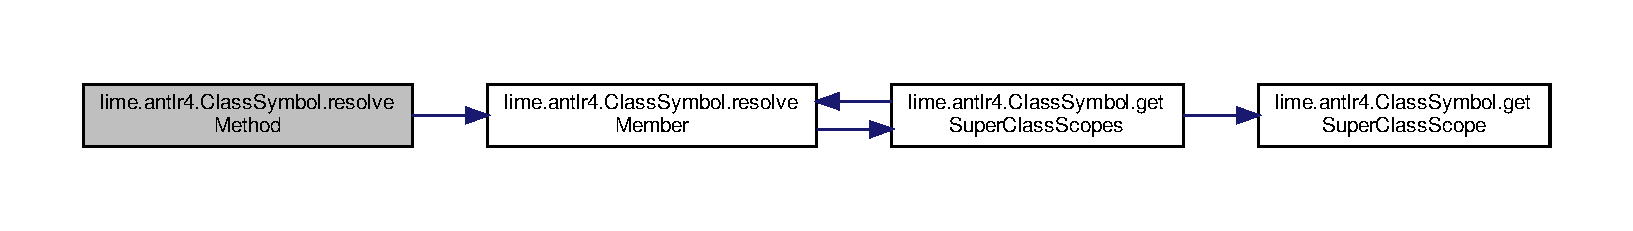
\includegraphics[width=350pt]{classlime_1_1antlr4_1_1ClassSymbol_a8b22f82d150b8c2fce1330ce7e570bb9_cgraph}
\end{center}
\end{figure}


The documentation for this class was generated from the following file\+:\begin{DoxyCompactItemize}
\item 
src/lime/antlr4/Class\+Symbol.\+java\end{DoxyCompactItemize}

\hypertarget{classlime_1_1antlr4_1_1DataAggregateSymbol}{}\section{lime.\+antlr4.\+Data\+Aggregate\+Symbol Class Reference}
\label{classlime_1_1antlr4_1_1DataAggregateSymbol}\index{lime.\+antlr4.\+Data\+Aggregate\+Symbol@{lime.\+antlr4.\+Data\+Aggregate\+Symbol}}


Inheritance diagram for lime.\+antlr4.\+Data\+Aggregate\+Symbol\+:
\nopagebreak
\begin{figure}[H]
\begin{center}
\leavevmode
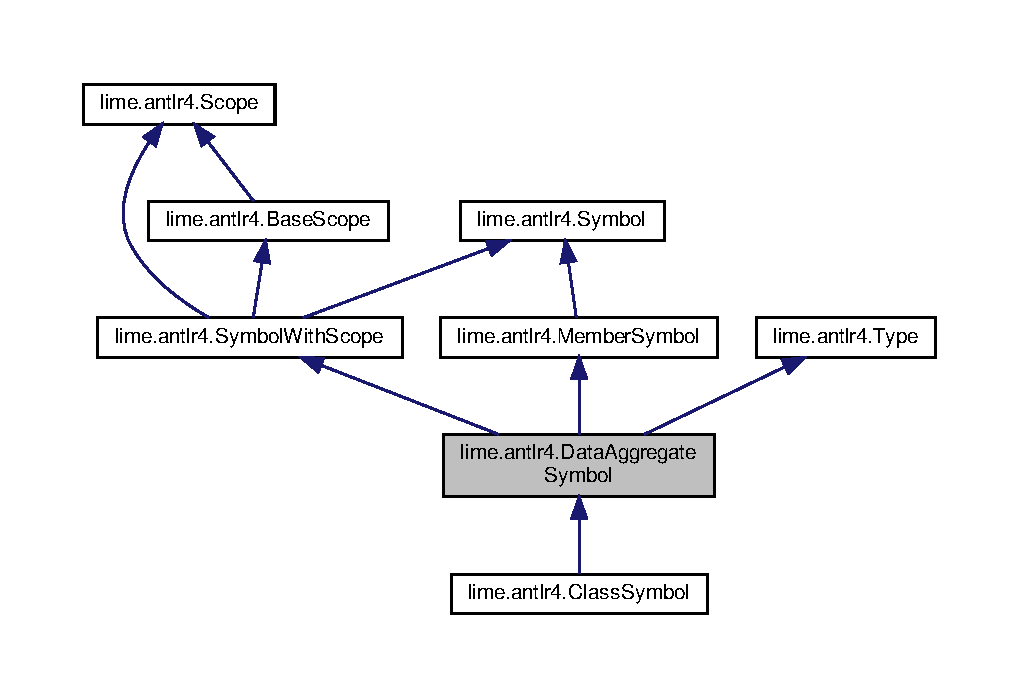
\includegraphics[width=350pt]{classlime_1_1antlr4_1_1DataAggregateSymbol__inherit__graph}
\end{center}
\end{figure}


Collaboration diagram for lime.\+antlr4.\+Data\+Aggregate\+Symbol\+:
\nopagebreak
\begin{figure}[H]
\begin{center}
\leavevmode
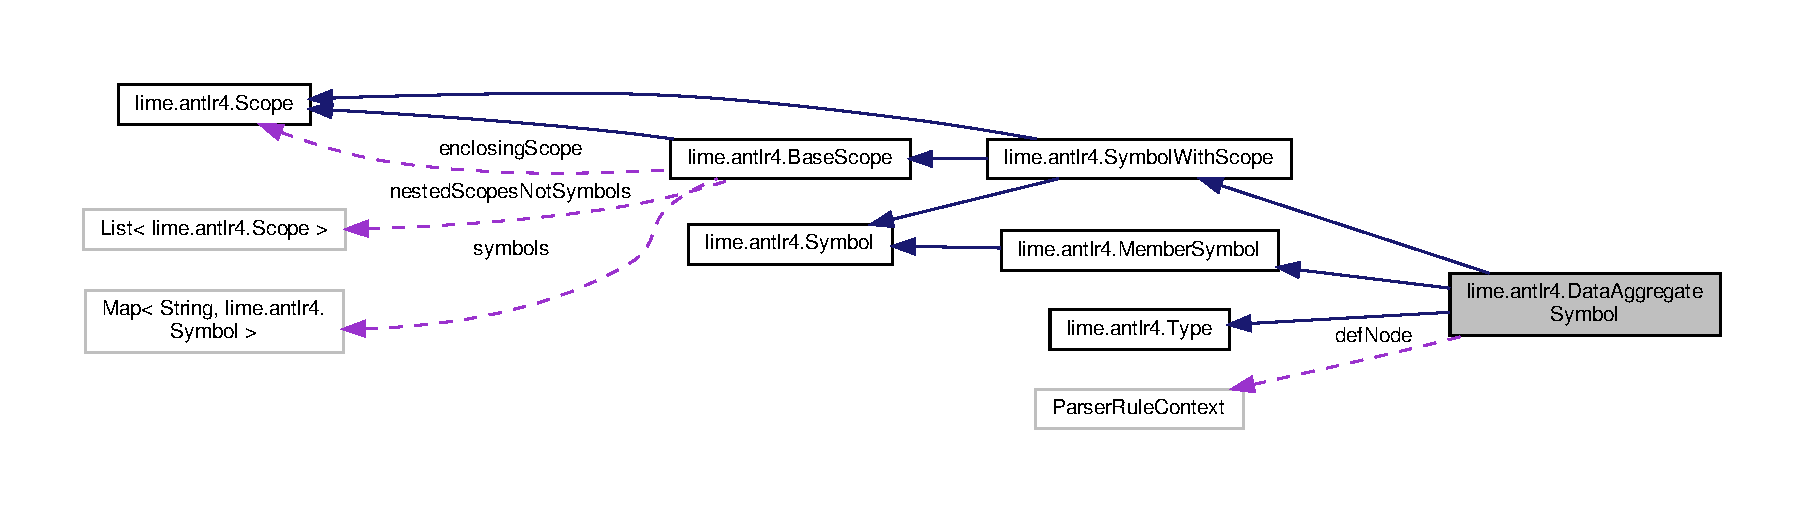
\includegraphics[width=350pt]{classlime_1_1antlr4_1_1DataAggregateSymbol__coll__graph}
\end{center}
\end{figure}
\subsection*{Public Member Functions}
\begin{DoxyCompactItemize}
\item 
\mbox{\Hypertarget{classlime_1_1antlr4_1_1DataAggregateSymbol_af5bc2cbf9f55353c0f3c4dfe68b37264}\label{classlime_1_1antlr4_1_1DataAggregateSymbol_af5bc2cbf9f55353c0f3c4dfe68b37264}} 
{\bfseries Data\+Aggregate\+Symbol} (String name)
\item 
\mbox{\Hypertarget{classlime_1_1antlr4_1_1DataAggregateSymbol_aa5b40e0ac8e54021bd945bb4a540bb87}\label{classlime_1_1antlr4_1_1DataAggregateSymbol_aa5b40e0ac8e54021bd945bb4a540bb87}} 
void {\bfseries set\+Def\+Node} (Parser\+Rule\+Context def\+Node)
\item 
\mbox{\Hypertarget{classlime_1_1antlr4_1_1DataAggregateSymbol_a9192b34aa0bfb8bf9fb557146758c50e}\label{classlime_1_1antlr4_1_1DataAggregateSymbol_a9192b34aa0bfb8bf9fb557146758c50e}} 
Parser\+Rule\+Context {\bfseries get\+Def\+Node} ()
\item 
\mbox{\Hypertarget{classlime_1_1antlr4_1_1DataAggregateSymbol_a801c13da5a9071f36d74644f342fc927}\label{classlime_1_1antlr4_1_1DataAggregateSymbol_a801c13da5a9071f36d74644f342fc927}} 
void {\bfseries define} (\hyperlink{interfacelime_1_1antlr4_1_1Symbol}{Symbol} sym)  throws Illegal\+Argument\+Exception 
\item 
\mbox{\Hypertarget{classlime_1_1antlr4_1_1DataAggregateSymbol_ad9a13cb3e8f8397e980c8ad352cceb4f}\label{classlime_1_1antlr4_1_1DataAggregateSymbol_ad9a13cb3e8f8397e980c8ad352cceb4f}} 
List$<$ \hyperlink{interfacelime_1_1antlr4_1_1MemberSymbol}{Member\+Symbol} $>$ {\bfseries get\+Symbols} ()
\item 
\mbox{\Hypertarget{classlime_1_1antlr4_1_1DataAggregateSymbol_aae39240cecab418ac71f51bd7404c4eb}\label{classlime_1_1antlr4_1_1DataAggregateSymbol_aae39240cecab418ac71f51bd7404c4eb}} 
Map$<$ String, ? extends \hyperlink{interfacelime_1_1antlr4_1_1MemberSymbol}{Member\+Symbol} $>$ {\bfseries get\+Members} ()
\item 
\hyperlink{interfacelime_1_1antlr4_1_1Symbol}{Symbol} \hyperlink{classlime_1_1antlr4_1_1DataAggregateSymbol_a59dd410b45c3761c12cff84c2bdb5a58}{resolve\+Member} (String name)
\item 
\hyperlink{interfacelime_1_1antlr4_1_1Symbol}{Symbol} \hyperlink{classlime_1_1antlr4_1_1DataAggregateSymbol_a0a1d90d6144f8c30e7733af041cc46f2}{resolve\+Field} (String name)
\item 
int \hyperlink{classlime_1_1antlr4_1_1DataAggregateSymbol_a80cf20fc8ae60730946f7dc2f1ab4a41}{get\+Number\+Of\+Defined\+Fields} ()
\item 
int \hyperlink{classlime_1_1antlr4_1_1DataAggregateSymbol_a12600a8ff3a06f489aa27ee91c9217bd}{get\+Number\+Of\+Fields} ()
\item 
List$<$? extends \hyperlink{classlime_1_1antlr4_1_1FieldSymbol}{Field\+Symbol} $>$ \hyperlink{classlime_1_1antlr4_1_1DataAggregateSymbol_abbb99b03010fbdccae19b976e79c468a}{get\+Defined\+Fields} ()
\item 
\mbox{\Hypertarget{classlime_1_1antlr4_1_1DataAggregateSymbol_a5b9ecf928da2dd6935702a045c6da293}\label{classlime_1_1antlr4_1_1DataAggregateSymbol_a5b9ecf928da2dd6935702a045c6da293}} 
List$<$? extends \hyperlink{classlime_1_1antlr4_1_1FieldSymbol}{Field\+Symbol} $>$ {\bfseries get\+Fields} ()
\item 
\mbox{\Hypertarget{classlime_1_1antlr4_1_1DataAggregateSymbol_ac83d1a71775a59209a623165aa1e21bf}\label{classlime_1_1antlr4_1_1DataAggregateSymbol_ac83d1a71775a59209a623165aa1e21bf}} 
void {\bfseries set\+Slot\+Number} (\hyperlink{interfacelime_1_1antlr4_1_1Symbol}{Symbol} sym)
\item 
\mbox{\Hypertarget{classlime_1_1antlr4_1_1DataAggregateSymbol_a6e3dc3797fa29f5cfcdfa4ddcf50c842}\label{classlime_1_1antlr4_1_1DataAggregateSymbol_a6e3dc3797fa29f5cfcdfa4ddcf50c842}} 
int {\bfseries get\+Slot\+Number} ()
\item 
\mbox{\Hypertarget{classlime_1_1antlr4_1_1DataAggregateSymbol_ae012c961e0e1dc6c1455166b52b815e6}\label{classlime_1_1antlr4_1_1DataAggregateSymbol_ae012c961e0e1dc6c1455166b52b815e6}} 
int {\bfseries get\+Type\+Index} ()
\item 
\mbox{\Hypertarget{classlime_1_1antlr4_1_1DataAggregateSymbol_ae2a3a658f2bd92c4825c94069c2413b5}\label{classlime_1_1antlr4_1_1DataAggregateSymbol_ae2a3a658f2bd92c4825c94069c2413b5}} 
void {\bfseries set\+Type\+Index} (int type\+Index)
\end{DoxyCompactItemize}
\subsection*{Protected Attributes}
\begin{DoxyCompactItemize}
\item 
\mbox{\Hypertarget{classlime_1_1antlr4_1_1DataAggregateSymbol_a13f4406e50faf421894a1f392d6d0f09}\label{classlime_1_1antlr4_1_1DataAggregateSymbol_a13f4406e50faf421894a1f392d6d0f09}} 
Parser\+Rule\+Context {\bfseries def\+Node}
\item 
\mbox{\Hypertarget{classlime_1_1antlr4_1_1DataAggregateSymbol_a1a0641836e8fb11ac9c6be114f05cc34}\label{classlime_1_1antlr4_1_1DataAggregateSymbol_a1a0641836e8fb11ac9c6be114f05cc34}} 
int {\bfseries next\+Free\+Field\+Slot} = 0
\item 
\mbox{\Hypertarget{classlime_1_1antlr4_1_1DataAggregateSymbol_ae526e41519f171ae95e591ec7bf0ddf1}\label{classlime_1_1antlr4_1_1DataAggregateSymbol_ae526e41519f171ae95e591ec7bf0ddf1}} 
int {\bfseries type\+Index}
\end{DoxyCompactItemize}


\subsection{Detailed Description}
A symbol representing a collection of data like a struct or class. Each member has a slot number indexed from 0 and we track data fields and methods with different slot sequences. A \hyperlink{classlime_1_1antlr4_1_1DataAggregateSymbol}{Data\+Aggregate\+Symbol} can also be a member of an aggregate itself (nested structs, ...). 

\subsection{Member Function Documentation}
\mbox{\Hypertarget{classlime_1_1antlr4_1_1DataAggregateSymbol_abbb99b03010fbdccae19b976e79c468a}\label{classlime_1_1antlr4_1_1DataAggregateSymbol_abbb99b03010fbdccae19b976e79c468a}} 
\index{lime\+::antlr4\+::\+Data\+Aggregate\+Symbol@{lime\+::antlr4\+::\+Data\+Aggregate\+Symbol}!get\+Defined\+Fields@{get\+Defined\+Fields}}
\index{get\+Defined\+Fields@{get\+Defined\+Fields}!lime\+::antlr4\+::\+Data\+Aggregate\+Symbol@{lime\+::antlr4\+::\+Data\+Aggregate\+Symbol}}
\subsubsection{\texorpdfstring{get\+Defined\+Fields()}{getDefinedFields()}}
{\footnotesize\ttfamily List$<$? extends \hyperlink{classlime_1_1antlr4_1_1FieldSymbol}{Field\+Symbol}$>$ lime.\+antlr4.\+Data\+Aggregate\+Symbol.\+get\+Defined\+Fields (\begin{DoxyParamCaption}{ }\end{DoxyParamCaption})}

Return the list of fields in this specific aggregate \mbox{\Hypertarget{classlime_1_1antlr4_1_1DataAggregateSymbol_a80cf20fc8ae60730946f7dc2f1ab4a41}\label{classlime_1_1antlr4_1_1DataAggregateSymbol_a80cf20fc8ae60730946f7dc2f1ab4a41}} 
\index{lime\+::antlr4\+::\+Data\+Aggregate\+Symbol@{lime\+::antlr4\+::\+Data\+Aggregate\+Symbol}!get\+Number\+Of\+Defined\+Fields@{get\+Number\+Of\+Defined\+Fields}}
\index{get\+Number\+Of\+Defined\+Fields@{get\+Number\+Of\+Defined\+Fields}!lime\+::antlr4\+::\+Data\+Aggregate\+Symbol@{lime\+::antlr4\+::\+Data\+Aggregate\+Symbol}}
\subsubsection{\texorpdfstring{get\+Number\+Of\+Defined\+Fields()}{getNumberOfDefinedFields()}}
{\footnotesize\ttfamily int lime.\+antlr4.\+Data\+Aggregate\+Symbol.\+get\+Number\+Of\+Defined\+Fields (\begin{DoxyParamCaption}{ }\end{DoxyParamCaption})}

get the number of fields defined specifically in this class \mbox{\Hypertarget{classlime_1_1antlr4_1_1DataAggregateSymbol_a12600a8ff3a06f489aa27ee91c9217bd}\label{classlime_1_1antlr4_1_1DataAggregateSymbol_a12600a8ff3a06f489aa27ee91c9217bd}} 
\index{lime\+::antlr4\+::\+Data\+Aggregate\+Symbol@{lime\+::antlr4\+::\+Data\+Aggregate\+Symbol}!get\+Number\+Of\+Fields@{get\+Number\+Of\+Fields}}
\index{get\+Number\+Of\+Fields@{get\+Number\+Of\+Fields}!lime\+::antlr4\+::\+Data\+Aggregate\+Symbol@{lime\+::antlr4\+::\+Data\+Aggregate\+Symbol}}
\subsubsection{\texorpdfstring{get\+Number\+Of\+Fields()}{getNumberOfFields()}}
{\footnotesize\ttfamily int lime.\+antlr4.\+Data\+Aggregate\+Symbol.\+get\+Number\+Of\+Fields (\begin{DoxyParamCaption}{ }\end{DoxyParamCaption})}

Get the total number of fields visible to this class Here is the call graph for this function\+:
\nopagebreak
\begin{figure}[H]
\begin{center}
\leavevmode
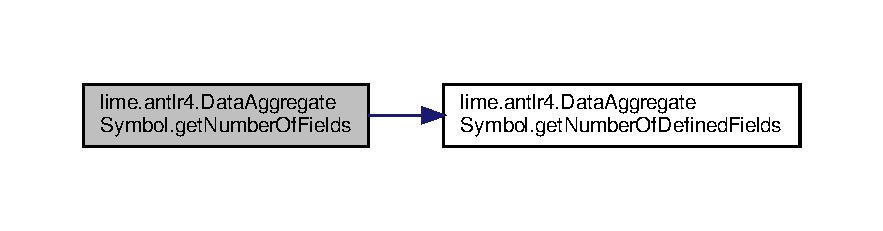
\includegraphics[width=350pt]{classlime_1_1antlr4_1_1DataAggregateSymbol_a12600a8ff3a06f489aa27ee91c9217bd_cgraph}
\end{center}
\end{figure}
\mbox{\Hypertarget{classlime_1_1antlr4_1_1DataAggregateSymbol_a0a1d90d6144f8c30e7733af041cc46f2}\label{classlime_1_1antlr4_1_1DataAggregateSymbol_a0a1d90d6144f8c30e7733af041cc46f2}} 
\index{lime\+::antlr4\+::\+Data\+Aggregate\+Symbol@{lime\+::antlr4\+::\+Data\+Aggregate\+Symbol}!resolve\+Field@{resolve\+Field}}
\index{resolve\+Field@{resolve\+Field}!lime\+::antlr4\+::\+Data\+Aggregate\+Symbol@{lime\+::antlr4\+::\+Data\+Aggregate\+Symbol}}
\subsubsection{\texorpdfstring{resolve\+Field()}{resolveField()}}
{\footnotesize\ttfamily \hyperlink{interfacelime_1_1antlr4_1_1Symbol}{Symbol} lime.\+antlr4.\+Data\+Aggregate\+Symbol.\+resolve\+Field (\begin{DoxyParamCaption}\item[{String}]{name }\end{DoxyParamCaption})}

Look for a field with this name in this scope only. Return null if no field found. Here is the call graph for this function\+:
\nopagebreak
\begin{figure}[H]
\begin{center}
\leavevmode
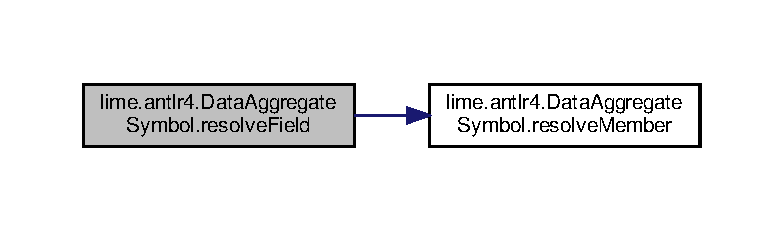
\includegraphics[width=350pt]{classlime_1_1antlr4_1_1DataAggregateSymbol_a0a1d90d6144f8c30e7733af041cc46f2_cgraph}
\end{center}
\end{figure}
\mbox{\Hypertarget{classlime_1_1antlr4_1_1DataAggregateSymbol_a59dd410b45c3761c12cff84c2bdb5a58}\label{classlime_1_1antlr4_1_1DataAggregateSymbol_a59dd410b45c3761c12cff84c2bdb5a58}} 
\index{lime\+::antlr4\+::\+Data\+Aggregate\+Symbol@{lime\+::antlr4\+::\+Data\+Aggregate\+Symbol}!resolve\+Member@{resolve\+Member}}
\index{resolve\+Member@{resolve\+Member}!lime\+::antlr4\+::\+Data\+Aggregate\+Symbol@{lime\+::antlr4\+::\+Data\+Aggregate\+Symbol}}
\subsubsection{\texorpdfstring{resolve\+Member()}{resolveMember()}}
{\footnotesize\ttfamily \hyperlink{interfacelime_1_1antlr4_1_1Symbol}{Symbol} lime.\+antlr4.\+Data\+Aggregate\+Symbol.\+resolve\+Member (\begin{DoxyParamCaption}\item[{String}]{name }\end{DoxyParamCaption})}

Look up name within this scope only. Return any kind of \hyperlink{interfacelime_1_1antlr4_1_1MemberSymbol}{Member\+Symbol} found or null if nothing with this name found as \hyperlink{interfacelime_1_1antlr4_1_1MemberSymbol}{Member\+Symbol}. 

The documentation for this class was generated from the following file\+:\begin{DoxyCompactItemize}
\item 
src/lime/antlr4/Data\+Aggregate\+Symbol.\+java\end{DoxyCompactItemize}

\hypertarget{classlime_1_1antlr4_1_1DescriptiveBailErrorListener}{}\section{lime.\+antlr4.\+Descriptive\+Bail\+Error\+Listener Class Reference}
\label{classlime_1_1antlr4_1_1DescriptiveBailErrorListener}\index{lime.\+antlr4.\+Descriptive\+Bail\+Error\+Listener@{lime.\+antlr4.\+Descriptive\+Bail\+Error\+Listener}}


Inheritance diagram for lime.\+antlr4.\+Descriptive\+Bail\+Error\+Listener\+:
\nopagebreak
\begin{figure}[H]
\begin{center}
\leavevmode
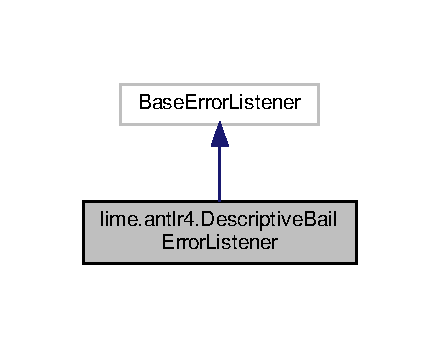
\includegraphics[width=211pt]{classlime_1_1antlr4_1_1DescriptiveBailErrorListener__inherit__graph}
\end{center}
\end{figure}


Collaboration diagram for lime.\+antlr4.\+Descriptive\+Bail\+Error\+Listener\+:
\nopagebreak
\begin{figure}[H]
\begin{center}
\leavevmode
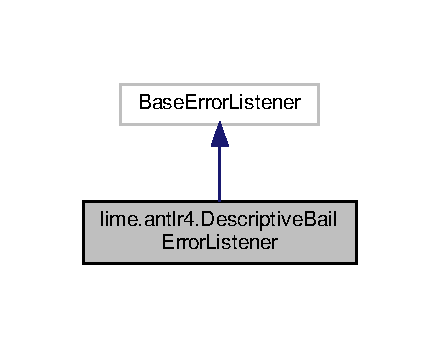
\includegraphics[width=211pt]{classlime_1_1antlr4_1_1DescriptiveBailErrorListener__coll__graph}
\end{center}
\end{figure}
\subsection*{Public Member Functions}
\begin{DoxyCompactItemize}
\item 
\mbox{\Hypertarget{classlime_1_1antlr4_1_1DescriptiveBailErrorListener_a88c7997d1d94ac3564a67d80b7b10780}\label{classlime_1_1antlr4_1_1DescriptiveBailErrorListener_a88c7997d1d94ac3564a67d80b7b10780}} 
void {\bfseries syntax\+Error} (Recognizer$<$?, ?$>$ recognizer, Object offending\+Symbol, int line, int char\+Position\+In\+Line, String msg, Recognition\+Exception e)
\end{DoxyCompactItemize}


\subsection{Detailed Description}
An error listener that immediately bails out of the parse (does not recover) and throws a runtime exception with a descriptive error message. 

The documentation for this class was generated from the following file\+:\begin{DoxyCompactItemize}
\item 
src/lime/antlr4/Descriptive\+Bail\+Error\+Listener.\+java\end{DoxyCompactItemize}

\hypertarget{classlime_1_1antlr4_1_1FieldSymbol}{}\section{lime.\+antlr4.\+Field\+Symbol Class Reference}
\label{classlime_1_1antlr4_1_1FieldSymbol}\index{lime.\+antlr4.\+Field\+Symbol@{lime.\+antlr4.\+Field\+Symbol}}


Inheritance diagram for lime.\+antlr4.\+Field\+Symbol\+:
\nopagebreak
\begin{figure}[H]
\begin{center}
\leavevmode
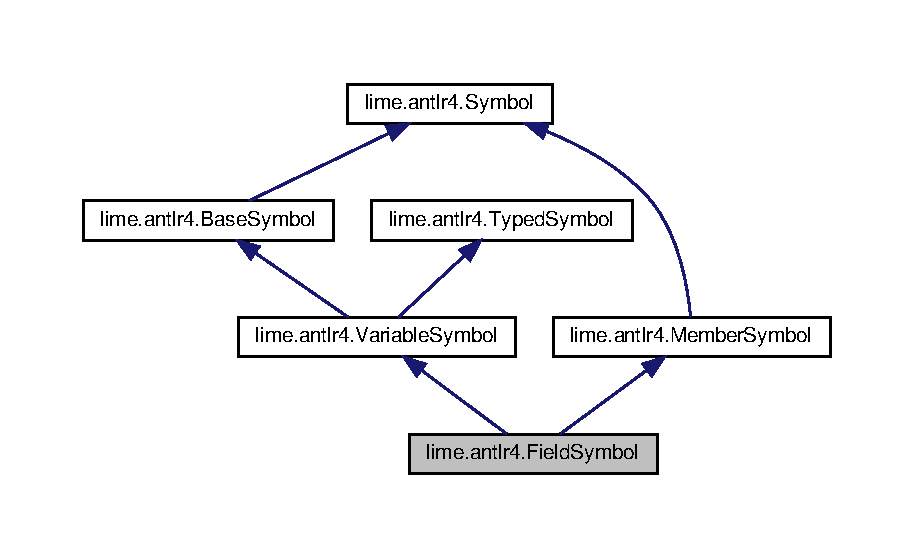
\includegraphics[width=350pt]{classlime_1_1antlr4_1_1FieldSymbol__inherit__graph}
\end{center}
\end{figure}


Collaboration diagram for lime.\+antlr4.\+Field\+Symbol\+:
\nopagebreak
\begin{figure}[H]
\begin{center}
\leavevmode
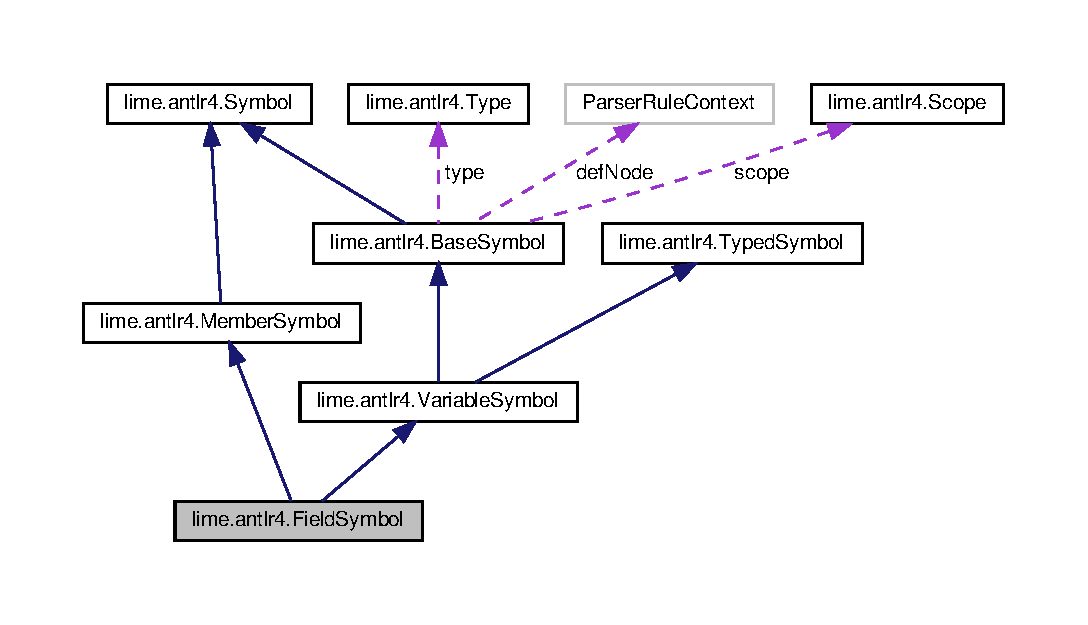
\includegraphics[width=350pt]{classlime_1_1antlr4_1_1FieldSymbol__coll__graph}
\end{center}
\end{figure}
\subsection*{Public Member Functions}
\begin{DoxyCompactItemize}
\item 
\mbox{\Hypertarget{classlime_1_1antlr4_1_1FieldSymbol_a717718bd57c2f6caeee12bfc0ba3374a}\label{classlime_1_1antlr4_1_1FieldSymbol_a717718bd57c2f6caeee12bfc0ba3374a}} 
{\bfseries Field\+Symbol} (String name)
\item 
\mbox{\Hypertarget{classlime_1_1antlr4_1_1FieldSymbol_a5ce9ad14aa8f9f11726ac4dc492f4d2e}\label{classlime_1_1antlr4_1_1FieldSymbol_a5ce9ad14aa8f9f11726ac4dc492f4d2e}} 
int {\bfseries get\+Slot\+Number} ()
\item 
\mbox{\Hypertarget{classlime_1_1antlr4_1_1FieldSymbol_a65e351376bb4ad9fd477dff778975c75}\label{classlime_1_1antlr4_1_1FieldSymbol_a65e351376bb4ad9fd477dff778975c75}} 
String {\bfseries to\+String} ()
\end{DoxyCompactItemize}
\subsection*{Protected Attributes}
\begin{DoxyCompactItemize}
\item 
\mbox{\Hypertarget{classlime_1_1antlr4_1_1FieldSymbol_a56c46907abe7bf78b27359efea2ec4b5}\label{classlime_1_1antlr4_1_1FieldSymbol_a56c46907abe7bf78b27359efea2ec4b5}} 
int {\bfseries slot}
\end{DoxyCompactItemize}


The documentation for this class was generated from the following file\+:\begin{DoxyCompactItemize}
\item 
src/lime/antlr4/Field\+Symbol.\+java\end{DoxyCompactItemize}

\hypertarget{classlime_1_1antlr4_1_1FunctionSymbol}{}\section{lime.\+antlr4.\+Function\+Symbol Class Reference}
\label{classlime_1_1antlr4_1_1FunctionSymbol}\index{lime.\+antlr4.\+Function\+Symbol@{lime.\+antlr4.\+Function\+Symbol}}


Inheritance diagram for lime.\+antlr4.\+Function\+Symbol\+:
\nopagebreak
\begin{figure}[H]
\begin{center}
\leavevmode
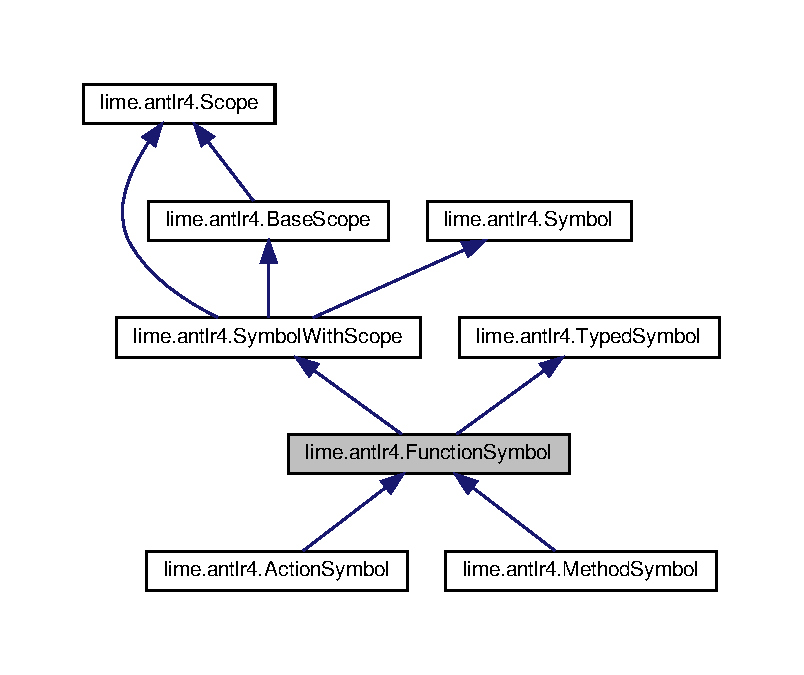
\includegraphics[width=350pt]{classlime_1_1antlr4_1_1FunctionSymbol__inherit__graph}
\end{center}
\end{figure}


Collaboration diagram for lime.\+antlr4.\+Function\+Symbol\+:
\nopagebreak
\begin{figure}[H]
\begin{center}
\leavevmode
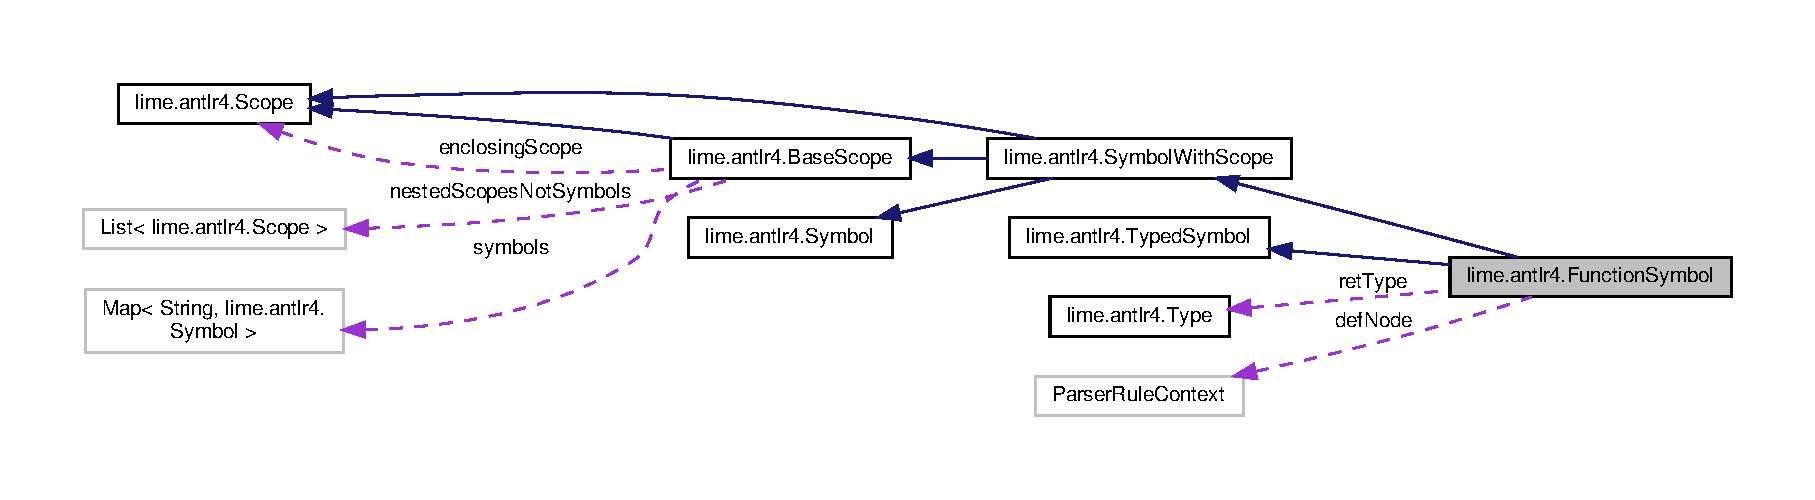
\includegraphics[width=350pt]{classlime_1_1antlr4_1_1FunctionSymbol__coll__graph}
\end{center}
\end{figure}
\subsection*{Public Member Functions}
\begin{DoxyCompactItemize}
\item 
\mbox{\Hypertarget{classlime_1_1antlr4_1_1FunctionSymbol_a791d85367a28923361df264837d1b18b}\label{classlime_1_1antlr4_1_1FunctionSymbol_a791d85367a28923361df264837d1b18b}} 
{\bfseries Function\+Symbol} (String name)
\item 
\mbox{\Hypertarget{classlime_1_1antlr4_1_1FunctionSymbol_a3c1784ebca6174caa72166a69ec6ea6d}\label{classlime_1_1antlr4_1_1FunctionSymbol_a3c1784ebca6174caa72166a69ec6ea6d}} 
void {\bfseries set\+Def\+Node} (Parser\+Rule\+Context def\+Node)
\item 
\mbox{\Hypertarget{classlime_1_1antlr4_1_1FunctionSymbol_a68a05aebca7b6a8f54e8860ee8f96786}\label{classlime_1_1antlr4_1_1FunctionSymbol_a68a05aebca7b6a8f54e8860ee8f96786}} 
Parser\+Rule\+Context {\bfseries get\+Def\+Node} ()
\item 
\mbox{\Hypertarget{classlime_1_1antlr4_1_1FunctionSymbol_a82fdb02d431544e19bac7cc032122028}\label{classlime_1_1antlr4_1_1FunctionSymbol_a82fdb02d431544e19bac7cc032122028}} 
\hyperlink{interfacelime_1_1antlr4_1_1Type}{Type} {\bfseries get\+Type} ()
\item 
\mbox{\Hypertarget{classlime_1_1antlr4_1_1FunctionSymbol_a671e7ea2964f0fddaa0e4091ee4446ef}\label{classlime_1_1antlr4_1_1FunctionSymbol_a671e7ea2964f0fddaa0e4091ee4446ef}} 
void {\bfseries set\+Type} (\hyperlink{interfacelime_1_1antlr4_1_1Type}{Type} type)
\item 
\mbox{\Hypertarget{classlime_1_1antlr4_1_1FunctionSymbol_a47a1895956658ef21768a2a3c28e2d81}\label{classlime_1_1antlr4_1_1FunctionSymbol_a47a1895956658ef21768a2a3c28e2d81}} 
int {\bfseries get\+Number\+Of\+Variables} ()
\item 
\mbox{\Hypertarget{classlime_1_1antlr4_1_1FunctionSymbol_aa73aac60215efc3ea9b5d6a304cfbc65}\label{classlime_1_1antlr4_1_1FunctionSymbol_aa73aac60215efc3ea9b5d6a304cfbc65}} 
int {\bfseries get\+Number\+Of\+Parameters} ()
\item 
\mbox{\Hypertarget{classlime_1_1antlr4_1_1FunctionSymbol_ac44145cd99893150d723906efafe4c0e}\label{classlime_1_1antlr4_1_1FunctionSymbol_ac44145cd99893150d723906efafe4c0e}} 
int {\bfseries get\+Par\+Index} (String p)
\item 
\mbox{\Hypertarget{classlime_1_1antlr4_1_1FunctionSymbol_a05d60f874472822a4fc02c1f44b2ff15}\label{classlime_1_1antlr4_1_1FunctionSymbol_a05d60f874472822a4fc02c1f44b2ff15}} 
String {\bfseries to\+String} ()
\end{DoxyCompactItemize}
\subsection*{Public Attributes}
\begin{DoxyCompactItemize}
\item 
\mbox{\Hypertarget{classlime_1_1antlr4_1_1FunctionSymbol_a334b65f24867b2427b964335e6124ac7}\label{classlime_1_1antlr4_1_1FunctionSymbol_a334b65f24867b2427b964335e6124ac7}} 
String {\bfseries guard}
\end{DoxyCompactItemize}
\subsection*{Protected Attributes}
\begin{DoxyCompactItemize}
\item 
\mbox{\Hypertarget{classlime_1_1antlr4_1_1FunctionSymbol_a003110d5ef39cc723fdf4df07527be8f}\label{classlime_1_1antlr4_1_1FunctionSymbol_a003110d5ef39cc723fdf4df07527be8f}} 
Parser\+Rule\+Context {\bfseries def\+Node}
\item 
\mbox{\Hypertarget{classlime_1_1antlr4_1_1FunctionSymbol_a55b846a3df1a738ef1b49f1216dbc61d}\label{classlime_1_1antlr4_1_1FunctionSymbol_a55b846a3df1a738ef1b49f1216dbc61d}} 
\hyperlink{interfacelime_1_1antlr4_1_1Type}{Type} {\bfseries ret\+Type}
\end{DoxyCompactItemize}


The documentation for this class was generated from the following file\+:\begin{DoxyCompactItemize}
\item 
src/lime/antlr4/Function\+Symbol.\+java\end{DoxyCompactItemize}

\hypertarget{classlime_1_1antlr4_1_1FunctionType}{}\section{lime.\+antlr4.\+Function\+Type Class Reference}
\label{classlime_1_1antlr4_1_1FunctionType}\index{lime.\+antlr4.\+Function\+Type@{lime.\+antlr4.\+Function\+Type}}


Inheritance diagram for lime.\+antlr4.\+Function\+Type\+:
\nopagebreak
\begin{figure}[H]
\begin{center}
\leavevmode
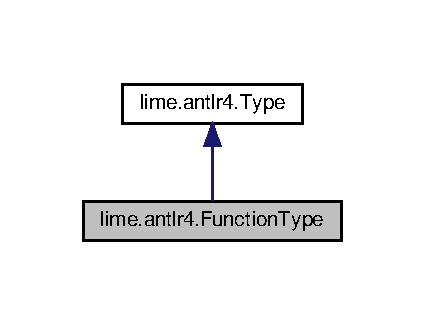
\includegraphics[width=204pt]{classlime_1_1antlr4_1_1FunctionType__inherit__graph}
\end{center}
\end{figure}


Collaboration diagram for lime.\+antlr4.\+Function\+Type\+:
\nopagebreak
\begin{figure}[H]
\begin{center}
\leavevmode
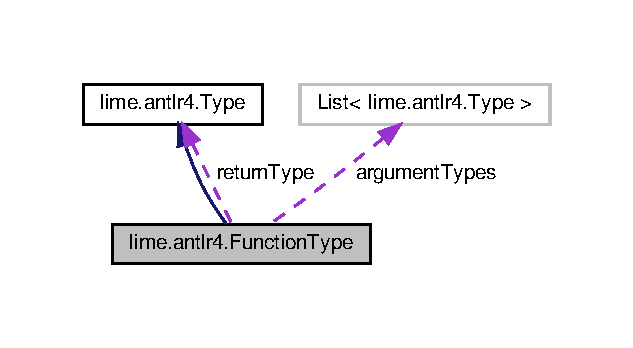
\includegraphics[width=304pt]{classlime_1_1antlr4_1_1FunctionType__coll__graph}
\end{center}
\end{figure}
\subsection*{Public Member Functions}
\begin{DoxyCompactItemize}
\item 
\mbox{\Hypertarget{classlime_1_1antlr4_1_1FunctionType_a1f9cf618ef349d75a9eb58d8a6c4d74d}\label{classlime_1_1antlr4_1_1FunctionType_a1f9cf618ef349d75a9eb58d8a6c4d74d}} 
{\bfseries Function\+Type} (\hyperlink{interfacelime_1_1antlr4_1_1Type}{Type} return\+Type, List$<$ \hyperlink{interfacelime_1_1antlr4_1_1Type}{Type} $>$ argument\+Types)
\item 
\mbox{\Hypertarget{classlime_1_1antlr4_1_1FunctionType_a4dffd0e94cb9e3f59d29752052e9852a}\label{classlime_1_1antlr4_1_1FunctionType_a4dffd0e94cb9e3f59d29752052e9852a}} 
String {\bfseries get\+Name} ()
\item 
\mbox{\Hypertarget{classlime_1_1antlr4_1_1FunctionType_a92f86a4aa69b7940a87702d9d610bc32}\label{classlime_1_1antlr4_1_1FunctionType_a92f86a4aa69b7940a87702d9d610bc32}} 
int {\bfseries get\+Type\+Index} ()
\item 
\mbox{\Hypertarget{classlime_1_1antlr4_1_1FunctionType_a82881cf0408cd2a28a30429933da2ac8}\label{classlime_1_1antlr4_1_1FunctionType_a82881cf0408cd2a28a30429933da2ac8}} 
List$<$ \hyperlink{interfacelime_1_1antlr4_1_1Type}{Type} $>$ {\bfseries get\+Argument\+Types} ()
\item 
\mbox{\Hypertarget{classlime_1_1antlr4_1_1FunctionType_a57a702a2873d1c973c846a2188482eec}\label{classlime_1_1antlr4_1_1FunctionType_a57a702a2873d1c973c846a2188482eec}} 
String {\bfseries to\+String} ()
\end{DoxyCompactItemize}
\subsection*{Protected Attributes}
\begin{DoxyCompactItemize}
\item 
\mbox{\Hypertarget{classlime_1_1antlr4_1_1FunctionType_a6b7392827b70ddb03b1ebc056dd97442}\label{classlime_1_1antlr4_1_1FunctionType_a6b7392827b70ddb03b1ebc056dd97442}} 
final \hyperlink{interfacelime_1_1antlr4_1_1Type}{Type} {\bfseries return\+Type}
\item 
\mbox{\Hypertarget{classlime_1_1antlr4_1_1FunctionType_ac595a5b819321345ae3f3e74acd8e57e}\label{classlime_1_1antlr4_1_1FunctionType_ac595a5b819321345ae3f3e74acd8e57e}} 
final List$<$ \hyperlink{interfacelime_1_1antlr4_1_1Type}{Type} $>$ {\bfseries argument\+Types}
\end{DoxyCompactItemize}


The documentation for this class was generated from the following file\+:\begin{DoxyCompactItemize}
\item 
src/lime/antlr4/Function\+Type.\+java\end{DoxyCompactItemize}

\hypertarget{classlime_1_1antlr4_1_1GlobalScope}{}\section{lime.\+antlr4.\+Global\+Scope Class Reference}
\label{classlime_1_1antlr4_1_1GlobalScope}\index{lime.\+antlr4.\+Global\+Scope@{lime.\+antlr4.\+Global\+Scope}}


Inheritance diagram for lime.\+antlr4.\+Global\+Scope\+:
\nopagebreak
\begin{figure}[H]
\begin{center}
\leavevmode
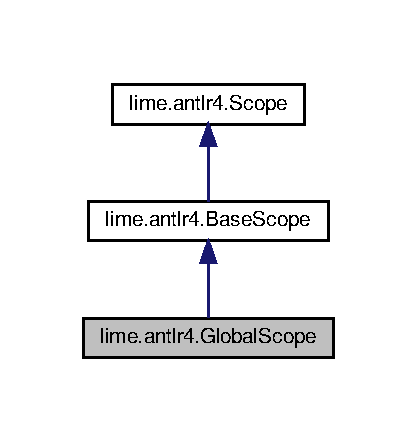
\includegraphics[width=200pt]{classlime_1_1antlr4_1_1GlobalScope__inherit__graph}
\end{center}
\end{figure}


Collaboration diagram for lime.\+antlr4.\+Global\+Scope\+:
\nopagebreak
\begin{figure}[H]
\begin{center}
\leavevmode
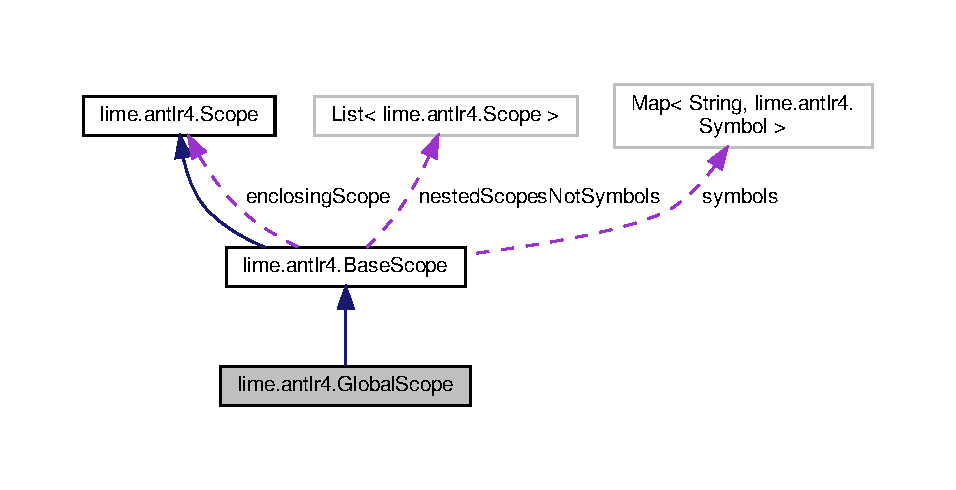
\includegraphics[width=350pt]{classlime_1_1antlr4_1_1GlobalScope__coll__graph}
\end{center}
\end{figure}
\subsection*{Public Member Functions}
\begin{DoxyCompactItemize}
\item 
\mbox{\Hypertarget{classlime_1_1antlr4_1_1GlobalScope_a045a91f24ac98ca4cd10b5d8d146cbd3}\label{classlime_1_1antlr4_1_1GlobalScope_a045a91f24ac98ca4cd10b5d8d146cbd3}} 
{\bfseries Global\+Scope} (\hyperlink{interfacelime_1_1antlr4_1_1Scope}{Scope} scope)
\item 
\mbox{\Hypertarget{classlime_1_1antlr4_1_1GlobalScope_a7499c2c0f470fabdf41ffb2228d0c606}\label{classlime_1_1antlr4_1_1GlobalScope_a7499c2c0f470fabdf41ffb2228d0c606}} 
String {\bfseries get\+Name} ()
\end{DoxyCompactItemize}
\subsection*{Additional Inherited Members}


The documentation for this class was generated from the following file\+:\begin{DoxyCompactItemize}
\item 
src/lime/antlr4/Global\+Scope.\+java\end{DoxyCompactItemize}

\hypertarget{classlime_1_1backend_1_1IntegerLiteral}{}\section{lime.\+backend.\+Integer\+Literal Class Reference}
\label{classlime_1_1backend_1_1IntegerLiteral}\index{lime.\+backend.\+Integer\+Literal@{lime.\+backend.\+Integer\+Literal}}


Inheritance diagram for lime.\+backend.\+Integer\+Literal\+:
\nopagebreak
\begin{figure}[H]
\begin{center}
\leavevmode
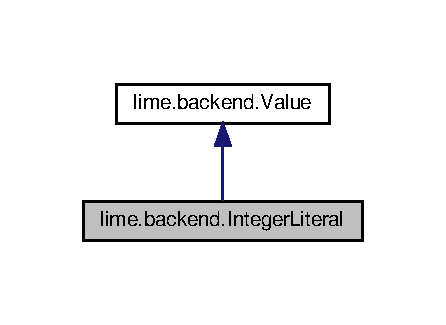
\includegraphics[width=214pt]{classlime_1_1backend_1_1IntegerLiteral__inherit__graph}
\end{center}
\end{figure}


Collaboration diagram for lime.\+backend.\+Integer\+Literal\+:
\nopagebreak
\begin{figure}[H]
\begin{center}
\leavevmode
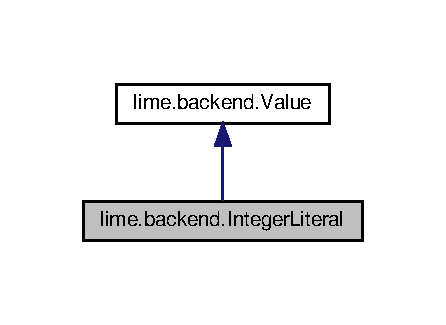
\includegraphics[width=214pt]{classlime_1_1backend_1_1IntegerLiteral__coll__graph}
\end{center}
\end{figure}
\subsection*{Public Member Functions}
\begin{DoxyCompactItemize}
\item 
\mbox{\Hypertarget{classlime_1_1backend_1_1IntegerLiteral_a1551d0bf66c6f0eb2a1508f1083ab752}\label{classlime_1_1backend_1_1IntegerLiteral_a1551d0bf66c6f0eb2a1508f1083ab752}} 
{\bfseries Integer\+Literal} (int i)
\item 
\mbox{\Hypertarget{classlime_1_1backend_1_1IntegerLiteral_a4a27afb9a39d6bacde2a15641d38471b}\label{classlime_1_1backend_1_1IntegerLiteral_a4a27afb9a39d6bacde2a15641d38471b}} 
String {\bfseries to\+String} ()
\end{DoxyCompactItemize}
\subsection*{Additional Inherited Members}


The documentation for this class was generated from the following file\+:\begin{DoxyCompactItemize}
\item 
src/lime/backend/Integer\+Literal.\+java\end{DoxyCompactItemize}

\hypertarget{classlime_1_1antlr4_1_1InvalidType}{}\section{lime.\+antlr4.\+Invalid\+Type Class Reference}
\label{classlime_1_1antlr4_1_1InvalidType}\index{lime.\+antlr4.\+Invalid\+Type@{lime.\+antlr4.\+Invalid\+Type}}


Inheritance diagram for lime.\+antlr4.\+Invalid\+Type\+:
\nopagebreak
\begin{figure}[H]
\begin{center}
\leavevmode
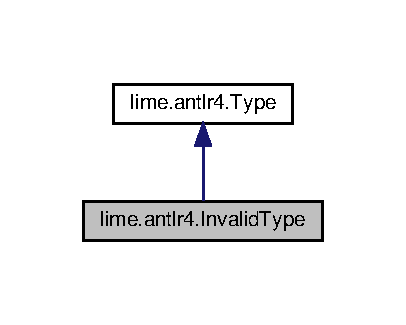
\includegraphics[width=195pt]{classlime_1_1antlr4_1_1InvalidType__inherit__graph}
\end{center}
\end{figure}


Collaboration diagram for lime.\+antlr4.\+Invalid\+Type\+:
\nopagebreak
\begin{figure}[H]
\begin{center}
\leavevmode
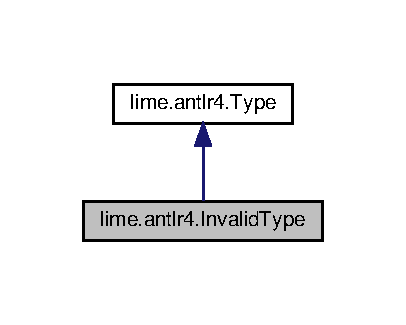
\includegraphics[width=195pt]{classlime_1_1antlr4_1_1InvalidType__coll__graph}
\end{center}
\end{figure}
\subsection*{Public Member Functions}
\begin{DoxyCompactItemize}
\item 
\mbox{\Hypertarget{classlime_1_1antlr4_1_1InvalidType_a51468b062a42f393646272823cbd7abe}\label{classlime_1_1antlr4_1_1InvalidType_a51468b062a42f393646272823cbd7abe}} 
String {\bfseries get\+Name} ()
\item 
\mbox{\Hypertarget{classlime_1_1antlr4_1_1InvalidType_a1fc1ab76a8844b317ef843f56d6b81ad}\label{classlime_1_1antlr4_1_1InvalidType_a1fc1ab76a8844b317ef843f56d6b81ad}} 
int {\bfseries get\+Type\+Index} ()
\end{DoxyCompactItemize}


The documentation for this class was generated from the following file\+:\begin{DoxyCompactItemize}
\item 
src/lime/antlr4/Invalid\+Type.\+java\end{DoxyCompactItemize}

\hypertarget{classlime_1_1codegen_1_1LimeLLVMCodeGenVisitor}{}\section{lime.\+codegen.\+Lime\+L\+L\+V\+M\+Code\+Gen\+Visitor Class Reference}
\label{classlime_1_1codegen_1_1LimeLLVMCodeGenVisitor}\index{lime.\+codegen.\+Lime\+L\+L\+V\+M\+Code\+Gen\+Visitor@{lime.\+codegen.\+Lime\+L\+L\+V\+M\+Code\+Gen\+Visitor}}


Inheritance diagram for lime.\+codegen.\+Lime\+L\+L\+V\+M\+Code\+Gen\+Visitor\+:
\nopagebreak
\begin{figure}[H]
\begin{center}
\leavevmode
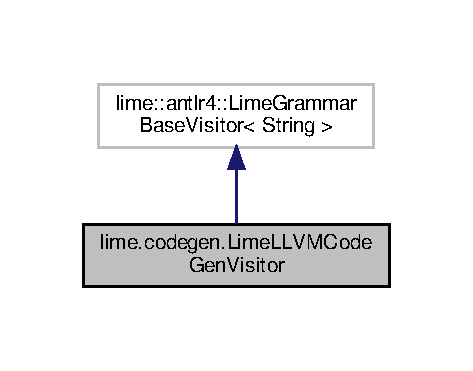
\includegraphics[width=227pt]{classlime_1_1codegen_1_1LimeLLVMCodeGenVisitor__inherit__graph}
\end{center}
\end{figure}


Collaboration diagram for lime.\+codegen.\+Lime\+L\+L\+V\+M\+Code\+Gen\+Visitor\+:
\nopagebreak
\begin{figure}[H]
\begin{center}
\leavevmode
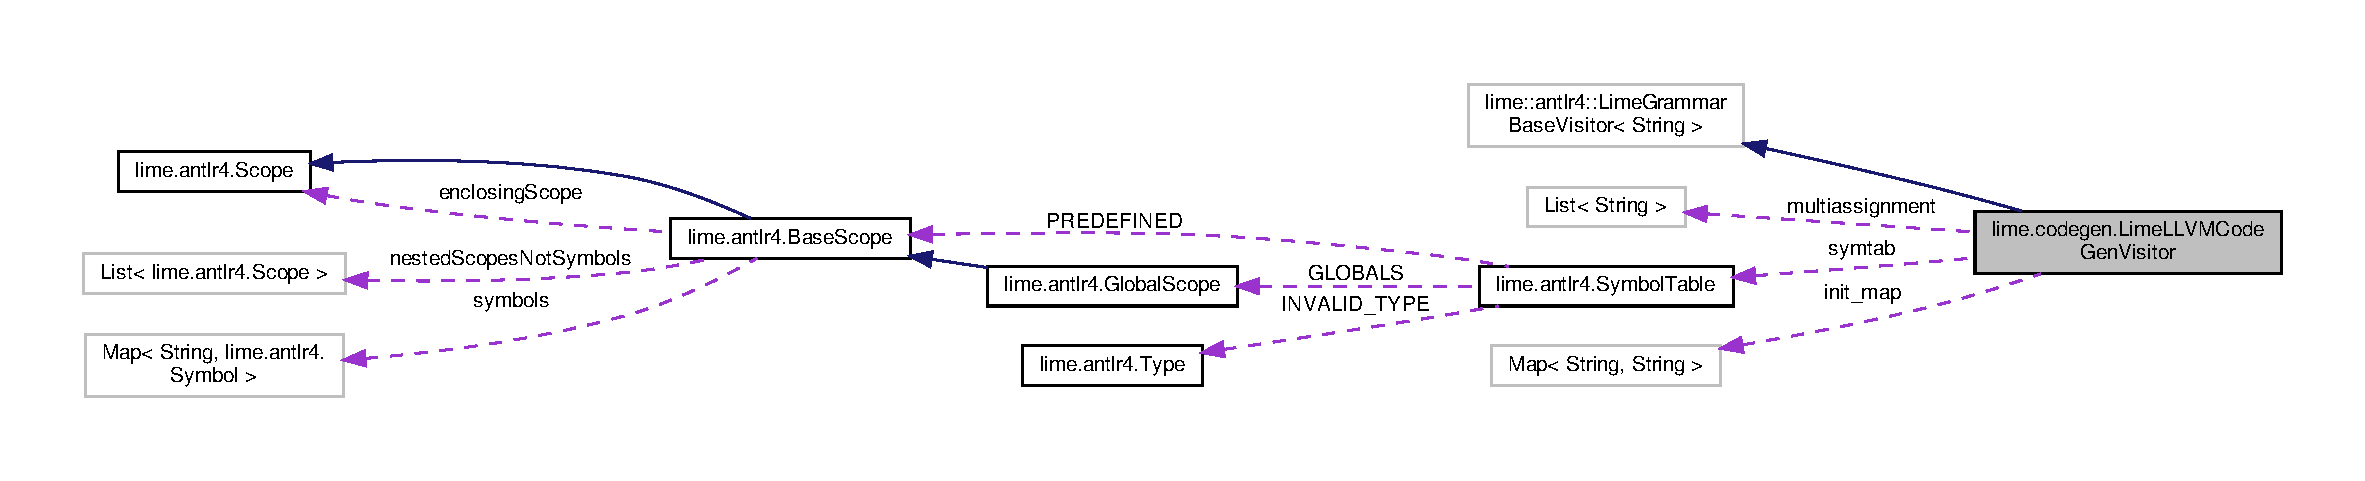
\includegraphics[width=350pt]{classlime_1_1codegen_1_1LimeLLVMCodeGenVisitor__coll__graph}
\end{center}
\end{figure}
\subsection*{Public Member Functions}
\begin{DoxyCompactItemize}
\item 
\mbox{\Hypertarget{classlime_1_1codegen_1_1LimeLLVMCodeGenVisitor_a434ccbda10d4427c8e0a349d317a5678}\label{classlime_1_1codegen_1_1LimeLLVMCodeGenVisitor_a434ccbda10d4427c8e0a349d317a5678}} 
{\bfseries Lime\+L\+L\+V\+M\+Code\+Gen\+Visitor} (\hyperlink{classlime_1_1antlr4_1_1SymbolTable}{Symbol\+Table} symtab)
\item 
\mbox{\Hypertarget{classlime_1_1codegen_1_1LimeLLVMCodeGenVisitor_a669f8c1ab46e5fa43385ef54ca3e76ba}\label{classlime_1_1codegen_1_1LimeLLVMCodeGenVisitor_a669f8c1ab46e5fa43385ef54ca3e76ba}} 
String {\bfseries visit\+Compilation\+Unit} (Compilation\+Unit\+Context ctx)
\item 
\mbox{\Hypertarget{classlime_1_1codegen_1_1LimeLLVMCodeGenVisitor_a1dd2209691c42022f55060da568dd80b}\label{classlime_1_1codegen_1_1LimeLLVMCodeGenVisitor_a1dd2209691c42022f55060da568dd80b}} 
String {\bfseries visit\+Class\+Decl} (Class\+Decl\+Context ctx)
\item 
\mbox{\Hypertarget{classlime_1_1codegen_1_1LimeLLVMCodeGenVisitor_a173105f9926c0a944468080335948c79}\label{classlime_1_1codegen_1_1LimeLLVMCodeGenVisitor_a173105f9926c0a944468080335948c79}} 
String {\bfseries visit\+Class\+Member} (Class\+Member\+Context ctx)
\item 
\mbox{\Hypertarget{classlime_1_1codegen_1_1LimeLLVMCodeGenVisitor_a5d74be722f08df7736056b24ac2dc057}\label{classlime_1_1codegen_1_1LimeLLVMCodeGenVisitor_a5d74be722f08df7736056b24ac2dc057}} 
String {\bfseries visit\+Init\+Decl} (Init\+Decl\+Context ctx)
\item 
\mbox{\Hypertarget{classlime_1_1codegen_1_1LimeLLVMCodeGenVisitor_a433b35880e5054003368a50d77a44c40}\label{classlime_1_1codegen_1_1LimeLLVMCodeGenVisitor_a433b35880e5054003368a50d77a44c40}} 
String {\bfseries visit\+Method\+Decl} (Method\+Decl\+Context ctx)
\item 
\mbox{\Hypertarget{classlime_1_1codegen_1_1LimeLLVMCodeGenVisitor_a2915ed6194823faf482226a0cb28a3bb}\label{classlime_1_1codegen_1_1LimeLLVMCodeGenVisitor_a2915ed6194823faf482226a0cb28a3bb}} 
String {\bfseries visit\+Parameters} (Parameters\+Context ctx)
\item 
\mbox{\Hypertarget{classlime_1_1codegen_1_1LimeLLVMCodeGenVisitor_a567c4740ca133174d0ad34cb03a05be7}\label{classlime_1_1codegen_1_1LimeLLVMCodeGenVisitor_a567c4740ca133174d0ad34cb03a05be7}} 
String {\bfseries visit\+Typeparslist} (Typeparslist\+Context ctx)
\item 
\mbox{\Hypertarget{classlime_1_1codegen_1_1LimeLLVMCodeGenVisitor_abc960b8bd27b956fecf73b792afe5f76}\label{classlime_1_1codegen_1_1LimeLLVMCodeGenVisitor_abc960b8bd27b956fecf73b792afe5f76}} 
String {\bfseries visit\+Parsdef} (Parsdef\+Context ctx)
\item 
\mbox{\Hypertarget{classlime_1_1codegen_1_1LimeLLVMCodeGenVisitor_a7ec7321ad919e81f14df57ff2f0de8f9}\label{classlime_1_1codegen_1_1LimeLLVMCodeGenVisitor_a7ec7321ad919e81f14df57ff2f0de8f9}} 
String {\bfseries visit\+Block} (Block\+Context ctx)
\item 
\mbox{\Hypertarget{classlime_1_1codegen_1_1LimeLLVMCodeGenVisitor_af6128669d68c00f7f760fe70df1e2b2c}\label{classlime_1_1codegen_1_1LimeLLVMCodeGenVisitor_af6128669d68c00f7f760fe70df1e2b2c}} 
String {\bfseries visit\+Stmt} (Stmt\+Context ctx)
\item 
\mbox{\Hypertarget{classlime_1_1codegen_1_1LimeLLVMCodeGenVisitor_ab1dbfca98cc9954b880c7629c0e429f6}\label{classlime_1_1codegen_1_1LimeLLVMCodeGenVisitor_ab1dbfca98cc9954b880c7629c0e429f6}} 
String {\bfseries visit\+Simple\+\_\+stmt} (Simple\+\_\+stmt\+Context ctx)
\item 
\mbox{\Hypertarget{classlime_1_1codegen_1_1LimeLLVMCodeGenVisitor_aa8c21276b1b57b08a8d7010b77c001b0}\label{classlime_1_1codegen_1_1LimeLLVMCodeGenVisitor_aa8c21276b1b57b08a8d7010b77c001b0}} 
String {\bfseries visit\+Small\+\_\+stmt} (Small\+\_\+stmt\+Context ctx)
\item 
\mbox{\Hypertarget{classlime_1_1codegen_1_1LimeLLVMCodeGenVisitor_aa7b85e187a360dd52ad665a14e80c6da}\label{classlime_1_1codegen_1_1LimeLLVMCodeGenVisitor_aa7b85e187a360dd52ad665a14e80c6da}} 
String {\bfseries visit\+Local\+Decl} (Local\+Decl\+Context ctx)
\item 
\mbox{\Hypertarget{classlime_1_1codegen_1_1LimeLLVMCodeGenVisitor_a09e1701af37806f98a80cb575d1246cb}\label{classlime_1_1codegen_1_1LimeLLVMCodeGenVisitor_a09e1701af37806f98a80cb575d1246cb}} 
String {\bfseries visit\+Multi\+\_\+assign} (Multi\+\_\+assign\+Context ctx)
\item 
\mbox{\Hypertarget{classlime_1_1codegen_1_1LimeLLVMCodeGenVisitor_a57d6076b302e156655cec0886f092cab}\label{classlime_1_1codegen_1_1LimeLLVMCodeGenVisitor_a57d6076b302e156655cec0886f092cab}} 
String {\bfseries visit\+Expr\+\_\+stmt} (Expr\+\_\+stmt\+Context ctx)
\item 
\mbox{\Hypertarget{classlime_1_1codegen_1_1LimeLLVMCodeGenVisitor_a3bf505142e5973423760585eaf02b0ac}\label{classlime_1_1codegen_1_1LimeLLVMCodeGenVisitor_a3bf505142e5973423760585eaf02b0ac}} 
String {\bfseries visit\+If\+\_\+stmt} (If\+\_\+stmt\+Context ctx)
\item 
\mbox{\Hypertarget{classlime_1_1codegen_1_1LimeLLVMCodeGenVisitor_a765c94238a8c9f021b714e12321535db}\label{classlime_1_1codegen_1_1LimeLLVMCodeGenVisitor_a765c94238a8c9f021b714e12321535db}} 
String {\bfseries visit\+If\+\_\+stat} (If\+\_\+stat\+Context ctx)
\item 
\mbox{\Hypertarget{classlime_1_1codegen_1_1LimeLLVMCodeGenVisitor_a737de37de4f711862cf3d19ee3487805}\label{classlime_1_1codegen_1_1LimeLLVMCodeGenVisitor_a737de37de4f711862cf3d19ee3487805}} 
String {\bfseries visit\+Elif\+\_\+stat} (Elif\+\_\+stat\+Context ctx)
\item 
\mbox{\Hypertarget{classlime_1_1codegen_1_1LimeLLVMCodeGenVisitor_a068ff46f07ea235f2859a05e52d29bc6}\label{classlime_1_1codegen_1_1LimeLLVMCodeGenVisitor_a068ff46f07ea235f2859a05e52d29bc6}} 
String {\bfseries visit\+Else\+\_\+stat} (Else\+\_\+stat\+Context ctx)
\item 
\mbox{\Hypertarget{classlime_1_1codegen_1_1LimeLLVMCodeGenVisitor_a248e4469d3e45c772c88432770f79f09}\label{classlime_1_1codegen_1_1LimeLLVMCodeGenVisitor_a248e4469d3e45c772c88432770f79f09}} 
String {\bfseries visit\+While\+\_\+stmt} (While\+\_\+stmt\+Context ctx)
\item 
\mbox{\Hypertarget{classlime_1_1codegen_1_1LimeLLVMCodeGenVisitor_a38ba452cc3833461c2676ba1a9a3ae75}\label{classlime_1_1codegen_1_1LimeLLVMCodeGenVisitor_a38ba452cc3833461c2676ba1a9a3ae75}} 
String {\bfseries visit\+Return\+\_\+stmt} (Return\+\_\+stmt\+Context ctx)
\item 
\mbox{\Hypertarget{classlime_1_1codegen_1_1LimeLLVMCodeGenVisitor_a6f47d26a3322eb335aa9aeb90a90e847}\label{classlime_1_1codegen_1_1LimeLLVMCodeGenVisitor_a6f47d26a3322eb335aa9aeb90a90e847}} 
String {\bfseries visit\+Action\+Decl} (Action\+Decl\+Context ctx)
\item 
\mbox{\Hypertarget{classlime_1_1codegen_1_1LimeLLVMCodeGenVisitor_a70ecf4d8013cd8cdc077dd9be516e424}\label{classlime_1_1codegen_1_1LimeLLVMCodeGenVisitor_a70ecf4d8013cd8cdc077dd9be516e424}} 
String {\bfseries visit\+Id\+\_\+list} (Id\+\_\+list\+Context ctx)
\item 
\mbox{\Hypertarget{classlime_1_1codegen_1_1LimeLLVMCodeGenVisitor_abd45dd8208270f2260cba41b731a60b2}\label{classlime_1_1codegen_1_1LimeLLVMCodeGenVisitor_abd45dd8208270f2260cba41b731a60b2}} 
String {\bfseries visit\+Eqexpr} (Eqexpr\+Context ctx)
\item 
\mbox{\Hypertarget{classlime_1_1codegen_1_1LimeLLVMCodeGenVisitor_a3a95d749df89f1002e0fbefb2c50d767}\label{classlime_1_1codegen_1_1LimeLLVMCodeGenVisitor_a3a95d749df89f1002e0fbefb2c50d767}} 
String {\bfseries visit\+Notexpr} (Notexpr\+Context ctx)
\item 
\mbox{\Hypertarget{classlime_1_1codegen_1_1LimeLLVMCodeGenVisitor_adc3e6d304b6c2b63bff7f5551d173e84}\label{classlime_1_1codegen_1_1LimeLLVMCodeGenVisitor_adc3e6d304b6c2b63bff7f5551d173e84}} 
String {\bfseries visit\+Multexpr} (Multexpr\+Context ctx)
\item 
\mbox{\Hypertarget{classlime_1_1codegen_1_1LimeLLVMCodeGenVisitor_a5e69f15a8550f6708cf4555d2068aed0}\label{classlime_1_1codegen_1_1LimeLLVMCodeGenVisitor_a5e69f15a8550f6708cf4555d2068aed0}} 
String {\bfseries visit\+Compexpr} (Compexpr\+Context ctx)
\item 
\mbox{\Hypertarget{classlime_1_1codegen_1_1LimeLLVMCodeGenVisitor_a25264b0103acccf455cee09f8e7c2bd8}\label{classlime_1_1codegen_1_1LimeLLVMCodeGenVisitor_a25264b0103acccf455cee09f8e7c2bd8}} 
String {\bfseries visit\+Unary\+Minusexpr} (Unary\+Minusexpr\+Context ctx)
\item 
\mbox{\Hypertarget{classlime_1_1codegen_1_1LimeLLVMCodeGenVisitor_ac31ea2abda943ec9ec929fd80a7b28ae}\label{classlime_1_1codegen_1_1LimeLLVMCodeGenVisitor_ac31ea2abda943ec9ec929fd80a7b28ae}} 
String {\bfseries visit\+Addexpr} (Addexpr\+Context ctx)
\item 
\mbox{\Hypertarget{classlime_1_1codegen_1_1LimeLLVMCodeGenVisitor_ac304ba13f36ae7f9af195cd36d13da65}\label{classlime_1_1codegen_1_1LimeLLVMCodeGenVisitor_ac304ba13f36ae7f9af195cd36d13da65}} 
String {\bfseries visit\+Atomexpr} (Atomexpr\+Context ctx)
\item 
\mbox{\Hypertarget{classlime_1_1codegen_1_1LimeLLVMCodeGenVisitor_aaae11315f7ba76c4ba35e3f8e5661f17}\label{classlime_1_1codegen_1_1LimeLLVMCodeGenVisitor_aaae11315f7ba76c4ba35e3f8e5661f17}} 
String {\bfseries visit\+Orexpr} (Orexpr\+Context ctx)
\item 
\mbox{\Hypertarget{classlime_1_1codegen_1_1LimeLLVMCodeGenVisitor_aa848b72dbf623bfd98d5d008acdeca33}\label{classlime_1_1codegen_1_1LimeLLVMCodeGenVisitor_aa848b72dbf623bfd98d5d008acdeca33}} 
String {\bfseries visit\+Andexpr} (Andexpr\+Context ctx)
\item 
\mbox{\Hypertarget{classlime_1_1codegen_1_1LimeLLVMCodeGenVisitor_abed40dfe78b35a86685c2ff51caa17db}\label{classlime_1_1codegen_1_1LimeLLVMCodeGenVisitor_abed40dfe78b35a86685c2ff51caa17db}} 
String {\bfseries visit\+Expr\+\_\+list} (Expr\+\_\+list\+Context ctx)
\item 
\mbox{\Hypertarget{classlime_1_1codegen_1_1LimeLLVMCodeGenVisitor_a85503ed6d48cdc366a6fcff3e6b4e4ee}\label{classlime_1_1codegen_1_1LimeLLVMCodeGenVisitor_a85503ed6d48cdc366a6fcff3e6b4e4ee}} 
String {\bfseries visit\+Newcall} (Newcall\+Context ctx)
\item 
\mbox{\Hypertarget{classlime_1_1codegen_1_1LimeLLVMCodeGenVisitor_a9b1d39c71e64d1c358e827cd6f799ba6}\label{classlime_1_1codegen_1_1LimeLLVMCodeGenVisitor_a9b1d39c71e64d1c358e827cd6f799ba6}} 
String {\bfseries visit\+Methodcall} (Methodcall\+Context ctx)
\item 
\mbox{\Hypertarget{classlime_1_1codegen_1_1LimeLLVMCodeGenVisitor_a98d37a702a5eed85607f570b257ed7f0}\label{classlime_1_1codegen_1_1LimeLLVMCodeGenVisitor_a98d37a702a5eed85607f570b257ed7f0}} 
String {\bfseries visit\+Args} (Args\+Context ctx)
\item 
\mbox{\Hypertarget{classlime_1_1codegen_1_1LimeLLVMCodeGenVisitor_af5d2d7e29e080f5fec2da5d965a42508}\label{classlime_1_1codegen_1_1LimeLLVMCodeGenVisitor_af5d2d7e29e080f5fec2da5d965a42508}} 
String {\bfseries visit\+Compound\+\_\+stmt} (Compound\+\_\+stmt\+Context ctx)
\item 
\mbox{\Hypertarget{classlime_1_1codegen_1_1LimeLLVMCodeGenVisitor_a29eed527a4bb21671463af9ffe9e63d6}\label{classlime_1_1codegen_1_1LimeLLVMCodeGenVisitor_a29eed527a4bb21671463af9ffe9e63d6}} 
String {\bfseries visit\+Atom} (Atom\+Context ctx)
\item 
\mbox{\Hypertarget{classlime_1_1codegen_1_1LimeLLVMCodeGenVisitor_a6d87ff843aecce85d70ac6c92e7247fb}\label{classlime_1_1codegen_1_1LimeLLVMCodeGenVisitor_a6d87ff843aecce85d70ac6c92e7247fb}} 
String {\bfseries to\+String} ()
\end{DoxyCompactItemize}


The documentation for this class was generated from the following file\+:\begin{DoxyCompactItemize}
\item 
src/lime/codegen/Lime\+L\+L\+V\+M\+Code\+Gen\+Visitor.\+java\end{DoxyCompactItemize}

\hypertarget{classlime_1_1codegen_1_1LimeParserTreeListener}{}\section{lime.\+codegen.\+Lime\+Parser\+Tree\+Listener Class Reference}
\label{classlime_1_1codegen_1_1LimeParserTreeListener}\index{lime.\+codegen.\+Lime\+Parser\+Tree\+Listener@{lime.\+codegen.\+Lime\+Parser\+Tree\+Listener}}


Inheritance diagram for lime.\+codegen.\+Lime\+Parser\+Tree\+Listener\+:
\nopagebreak
\begin{figure}[H]
\begin{center}
\leavevmode
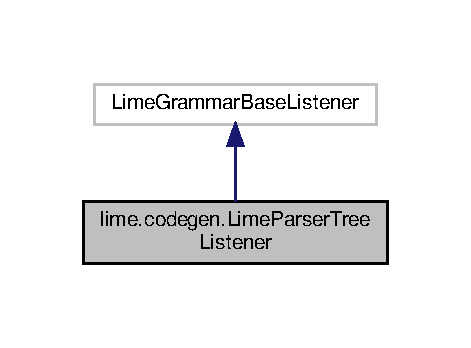
\includegraphics[width=226pt]{classlime_1_1codegen_1_1LimeParserTreeListener__inherit__graph}
\end{center}
\end{figure}


Collaboration diagram for lime.\+codegen.\+Lime\+Parser\+Tree\+Listener\+:
\nopagebreak
\begin{figure}[H]
\begin{center}
\leavevmode
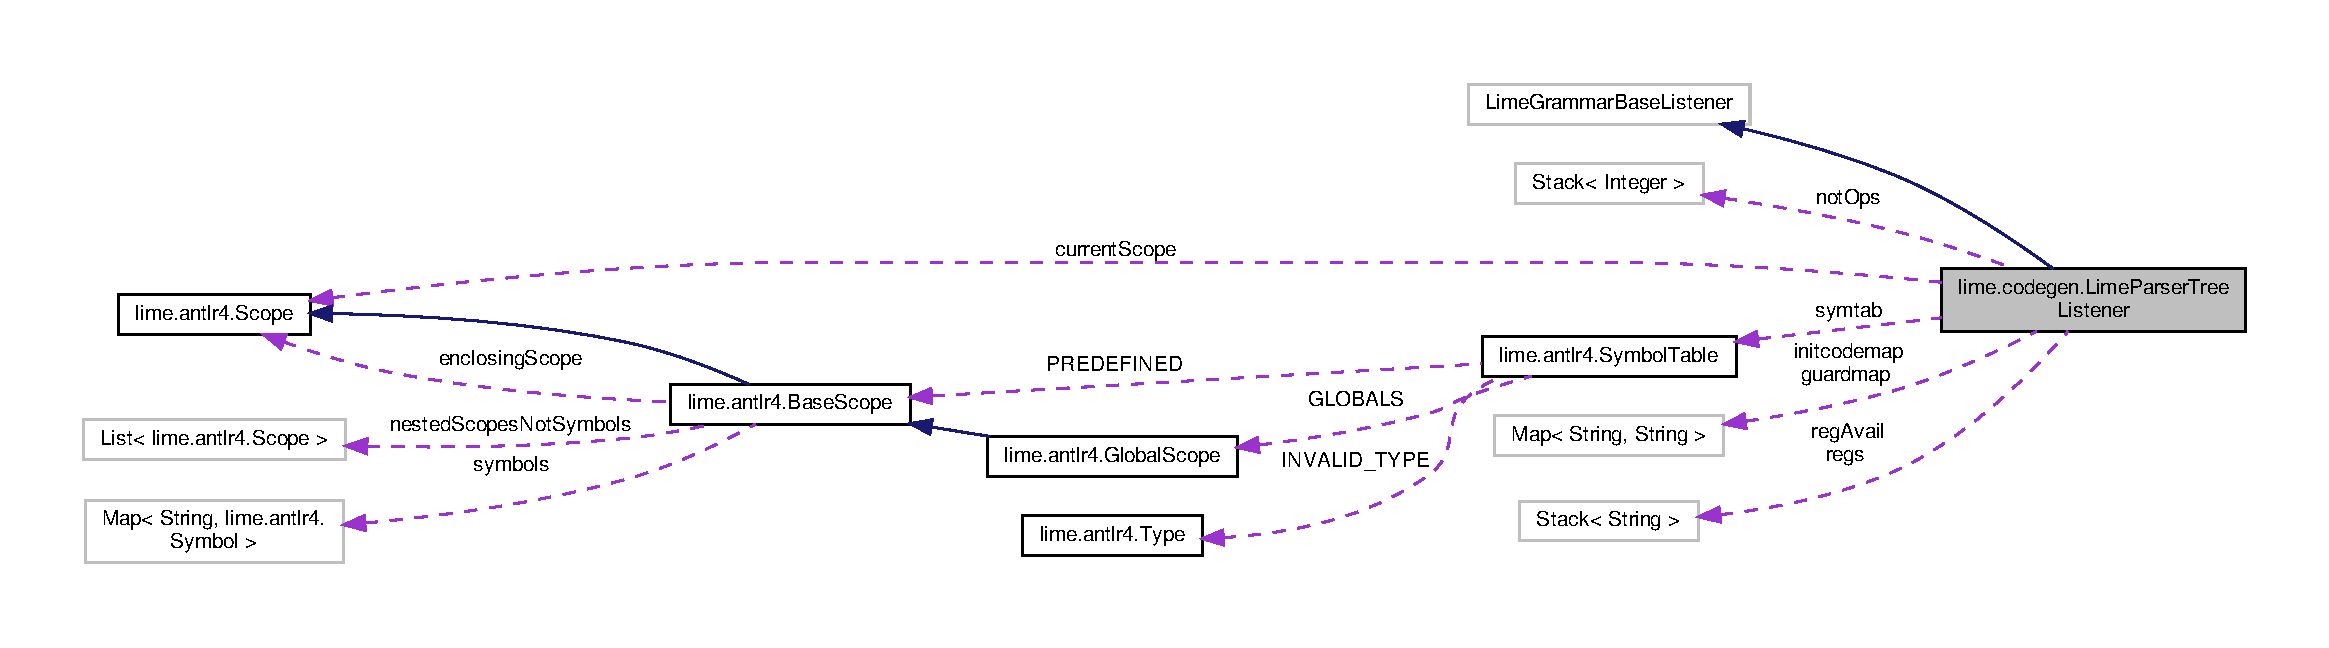
\includegraphics[width=350pt]{classlime_1_1codegen_1_1LimeParserTreeListener__coll__graph}
\end{center}
\end{figure}
\subsection*{Public Member Functions}
\begin{DoxyCompactItemize}
\item 
\mbox{\Hypertarget{classlime_1_1codegen_1_1LimeParserTreeListener_a5e7388d04f1df9d5b087c17baed52d61}\label{classlime_1_1codegen_1_1LimeParserTreeListener_a5e7388d04f1df9d5b087c17baed52d61}} 
{\bfseries Lime\+Parser\+Tree\+Listener} (\hyperlink{classlime_1_1antlr4_1_1SymbolTable}{Symbol\+Table} symtab)
\item 
\mbox{\Hypertarget{classlime_1_1codegen_1_1LimeParserTreeListener_aa4f8813ab29daaa5236bd9991a7d616d}\label{classlime_1_1codegen_1_1LimeParserTreeListener_aa4f8813ab29daaa5236bd9991a7d616d}} 
void {\bfseries enter\+Class\+Decl} (Class\+Decl\+Context ctx)
\item 
\mbox{\Hypertarget{classlime_1_1codegen_1_1LimeParserTreeListener_a797d03990c65915dfce9c5b782cfe86b}\label{classlime_1_1codegen_1_1LimeParserTreeListener_a797d03990c65915dfce9c5b782cfe86b}} 
void {\bfseries enter\+Compilation\+Unit} (Compilation\+Unit\+Context ctx)
\item 
\mbox{\Hypertarget{classlime_1_1codegen_1_1LimeParserTreeListener_a821f7e7fcf630f538dcf07808a09f3d1}\label{classlime_1_1codegen_1_1LimeParserTreeListener_a821f7e7fcf630f538dcf07808a09f3d1}} 
void {\bfseries exit\+Compilation\+Unit} (Compilation\+Unit\+Context ctx)
\item 
\mbox{\Hypertarget{classlime_1_1codegen_1_1LimeParserTreeListener_a046c2197b97fe2b614c12df71460ec92}\label{classlime_1_1codegen_1_1LimeParserTreeListener_a046c2197b97fe2b614c12df71460ec92}} 
void {\bfseries exit\+Class\+Decl} (Class\+Decl\+Context ctx)
\item 
\mbox{\Hypertarget{classlime_1_1codegen_1_1LimeParserTreeListener_ac7ab7da6c628d92cfdd7166998e71bd6}\label{classlime_1_1codegen_1_1LimeParserTreeListener_ac7ab7da6c628d92cfdd7166998e71bd6}} 
void {\bfseries enter\+Method\+Decl} (Method\+Decl\+Context ctx)
\item 
\mbox{\Hypertarget{classlime_1_1codegen_1_1LimeParserTreeListener_a409aded2df99e0b19b10fc1c53d63c07}\label{classlime_1_1codegen_1_1LimeParserTreeListener_a409aded2df99e0b19b10fc1c53d63c07}} 
void {\bfseries exit\+Method\+Decl} (Method\+Decl\+Context ctx)
\item 
\mbox{\Hypertarget{classlime_1_1codegen_1_1LimeParserTreeListener_a3ec823b85f639d3f6beb2ca33ef6cae4}\label{classlime_1_1codegen_1_1LimeParserTreeListener_a3ec823b85f639d3f6beb2ca33ef6cae4}} 
void {\bfseries enter\+Action\+Decl} (Action\+Decl\+Context ctx)
\item 
\mbox{\Hypertarget{classlime_1_1codegen_1_1LimeParserTreeListener_a89cfcd63d077ea36fde27a24f5dc6626}\label{classlime_1_1codegen_1_1LimeParserTreeListener_a89cfcd63d077ea36fde27a24f5dc6626}} 
void {\bfseries exit\+Action\+Decl} (Action\+Decl\+Context ctx)
\item 
\mbox{\Hypertarget{classlime_1_1codegen_1_1LimeParserTreeListener_abeca57cb27890df6e4f4f8ebeb001d4b}\label{classlime_1_1codegen_1_1LimeParserTreeListener_abeca57cb27890df6e4f4f8ebeb001d4b}} 
void {\bfseries enter\+Field\+Decl} (Field\+Decl\+Context ctx)
\item 
\mbox{\Hypertarget{classlime_1_1codegen_1_1LimeParserTreeListener_adacc586fdd70617fdbfa9b0eb19ee83b}\label{classlime_1_1codegen_1_1LimeParserTreeListener_adacc586fdd70617fdbfa9b0eb19ee83b}} 
boolean {\bfseries is\+Numeric} (String s)
\item 
\mbox{\Hypertarget{classlime_1_1codegen_1_1LimeParserTreeListener_ad71ab6015cc101630138734af3332b26}\label{classlime_1_1codegen_1_1LimeParserTreeListener_ad71ab6015cc101630138734af3332b26}} 
void {\bfseries enter\+Init\+Decl} (Init\+Decl\+Context ctx)
\item 
\mbox{\Hypertarget{classlime_1_1codegen_1_1LimeParserTreeListener_afbf33ffc149200a6efef8b8af851b140}\label{classlime_1_1codegen_1_1LimeParserTreeListener_afbf33ffc149200a6efef8b8af851b140}} 
void {\bfseries exit\+Init\+Decl} (Init\+Decl\+Context ctx)
\item 
\mbox{\Hypertarget{classlime_1_1codegen_1_1LimeParserTreeListener_ad0363aa2d6b1737cc81ae20d768c2271}\label{classlime_1_1codegen_1_1LimeParserTreeListener_ad0363aa2d6b1737cc81ae20d768c2271}} 
void {\bfseries enter\+Multi\+\_\+assign} (Multi\+\_\+assign\+Context ctx)
\item 
\mbox{\Hypertarget{classlime_1_1codegen_1_1LimeParserTreeListener_a13581d02098228204c0432478985cb42}\label{classlime_1_1codegen_1_1LimeParserTreeListener_a13581d02098228204c0432478985cb42}} 
void {\bfseries enter\+Parsdef} (Parsdef\+Context ctx)
\item 
\mbox{\Hypertarget{classlime_1_1codegen_1_1LimeParserTreeListener_a9de25e7eed4ab1f91d32781c4bbeaf7d}\label{classlime_1_1codegen_1_1LimeParserTreeListener_a9de25e7eed4ab1f91d32781c4bbeaf7d}} 
void {\bfseries enter\+Local\+Decl} (Local\+Decl\+Context ctx)
\item 
\mbox{\Hypertarget{classlime_1_1codegen_1_1LimeParserTreeListener_a5f783fba9a83862c7a80e7ae68d5ef69}\label{classlime_1_1codegen_1_1LimeParserTreeListener_a5f783fba9a83862c7a80e7ae68d5ef69}} 
void {\bfseries exit\+Guardcompexpr} (Guardcompexpr\+Context ctx)
\item 
\mbox{\Hypertarget{classlime_1_1codegen_1_1LimeParserTreeListener_a5aa4aab3a319bce6d6830214b5c6943e}\label{classlime_1_1codegen_1_1LimeParserTreeListener_a5aa4aab3a319bce6d6830214b5c6943e}} 
void {\bfseries exit\+Guardeqexpr} (Guardeqexpr\+Context ctx)
\item 
\mbox{\Hypertarget{classlime_1_1codegen_1_1LimeParserTreeListener_a43962e09f00f77cdcafbc6a02f00befd}\label{classlime_1_1codegen_1_1LimeParserTreeListener_a43962e09f00f77cdcafbc6a02f00befd}} 
void {\bfseries exit\+Guardandexpr} (Guardandexpr\+Context ctx)
\item 
\mbox{\Hypertarget{classlime_1_1codegen_1_1LimeParserTreeListener_ab30416a239bb412184a77739c0a8f42c}\label{classlime_1_1codegen_1_1LimeParserTreeListener_ab30416a239bb412184a77739c0a8f42c}} 
void {\bfseries exit\+Guardorexpr} (Guardorexpr\+Context ctx)
\item 
\mbox{\Hypertarget{classlime_1_1codegen_1_1LimeParserTreeListener_aba2f448e37720f9e68664c88d802cc6f}\label{classlime_1_1codegen_1_1LimeParserTreeListener_aba2f448e37720f9e68664c88d802cc6f}} 
void {\bfseries exit\+Guardatomexpr} (Guardatomexpr\+Context ctx)
\item 
\mbox{\Hypertarget{classlime_1_1codegen_1_1LimeParserTreeListener_ab826d9a1a52501e56c389c133b716710}\label{classlime_1_1codegen_1_1LimeParserTreeListener_ab826d9a1a52501e56c389c133b716710}} 
void {\bfseries exit\+Idguardatom} (Idguardatom\+Context ctx)
\item 
\mbox{\Hypertarget{classlime_1_1codegen_1_1LimeParserTreeListener_ab186f07607a1726bbaa8a746d21dac1c}\label{classlime_1_1codegen_1_1LimeParserTreeListener_ab186f07607a1726bbaa8a746d21dac1c}} 
void {\bfseries exit\+Intguardatom} (Intguardatom\+Context ctx)
\item 
\mbox{\Hypertarget{classlime_1_1codegen_1_1LimeParserTreeListener_a2c7958b467f69867411d16c2375aee3a}\label{classlime_1_1codegen_1_1LimeParserTreeListener_a2c7958b467f69867411d16c2375aee3a}} 
void {\bfseries exit\+Notguardtom} (Notguardtom\+Context ctx)
\item 
\mbox{\Hypertarget{classlime_1_1codegen_1_1LimeParserTreeListener_a49143095103c9cadc34425f34f042575}\label{classlime_1_1codegen_1_1LimeParserTreeListener_a49143095103c9cadc34425f34f042575}} 
void {\bfseries enter\+Atom} (Atom\+Context ctx)
\item 
\mbox{\Hypertarget{classlime_1_1codegen_1_1LimeParserTreeListener_a0ba963e73dd5eafffba9653cdc049d9d}\label{classlime_1_1codegen_1_1LimeParserTreeListener_a0ba963e73dd5eafffba9653cdc049d9d}} 
void {\bfseries enter\+Newcall} (Newcall\+Context ctx)
\item 
\mbox{\Hypertarget{classlime_1_1codegen_1_1LimeParserTreeListener_a50074b825bbaaf6a53a9c75929e6776a}\label{classlime_1_1codegen_1_1LimeParserTreeListener_a50074b825bbaaf6a53a9c75929e6776a}} 
void {\bfseries enter\+Methodcall} (Methodcall\+Context ctx)
\end{DoxyCompactItemize}
\subsection*{Public Attributes}
\begin{DoxyCompactItemize}
\item 
\mbox{\Hypertarget{classlime_1_1codegen_1_1LimeParserTreeListener_a2935cbe639237155e0162d5e0293edb1}\label{classlime_1_1codegen_1_1LimeParserTreeListener_a2935cbe639237155e0162d5e0293edb1}} 
Map$<$ String, String $>$ {\bfseries guardmap}
\item 
\mbox{\Hypertarget{classlime_1_1codegen_1_1LimeParserTreeListener_a15ac41818f9bcd2e054cf88348c33a08}\label{classlime_1_1codegen_1_1LimeParserTreeListener_a15ac41818f9bcd2e054cf88348c33a08}} 
Map$<$ String, String $>$ {\bfseries initcodemap}
\end{DoxyCompactItemize}


The documentation for this class was generated from the following file\+:\begin{DoxyCompactItemize}
\item 
src/lime/codegen/Lime\+Parser\+Tree\+Listener.\+java\end{DoxyCompactItemize}

\hypertarget{classlime_1_1codegen_1_1LimeSkeCodeGenListener}{}\section{lime.\+codegen.\+Lime\+Ske\+Code\+Gen\+Listener Class Reference}
\label{classlime_1_1codegen_1_1LimeSkeCodeGenListener}\index{lime.\+codegen.\+Lime\+Ske\+Code\+Gen\+Listener@{lime.\+codegen.\+Lime\+Ske\+Code\+Gen\+Listener}}


Inheritance diagram for lime.\+codegen.\+Lime\+Ske\+Code\+Gen\+Listener\+:
\nopagebreak
\begin{figure}[H]
\begin{center}
\leavevmode
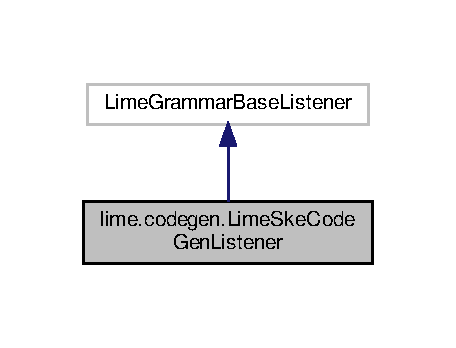
\includegraphics[width=219pt]{classlime_1_1codegen_1_1LimeSkeCodeGenListener__inherit__graph}
\end{center}
\end{figure}


Collaboration diagram for lime.\+codegen.\+Lime\+Ske\+Code\+Gen\+Listener\+:
\nopagebreak
\begin{figure}[H]
\begin{center}
\leavevmode
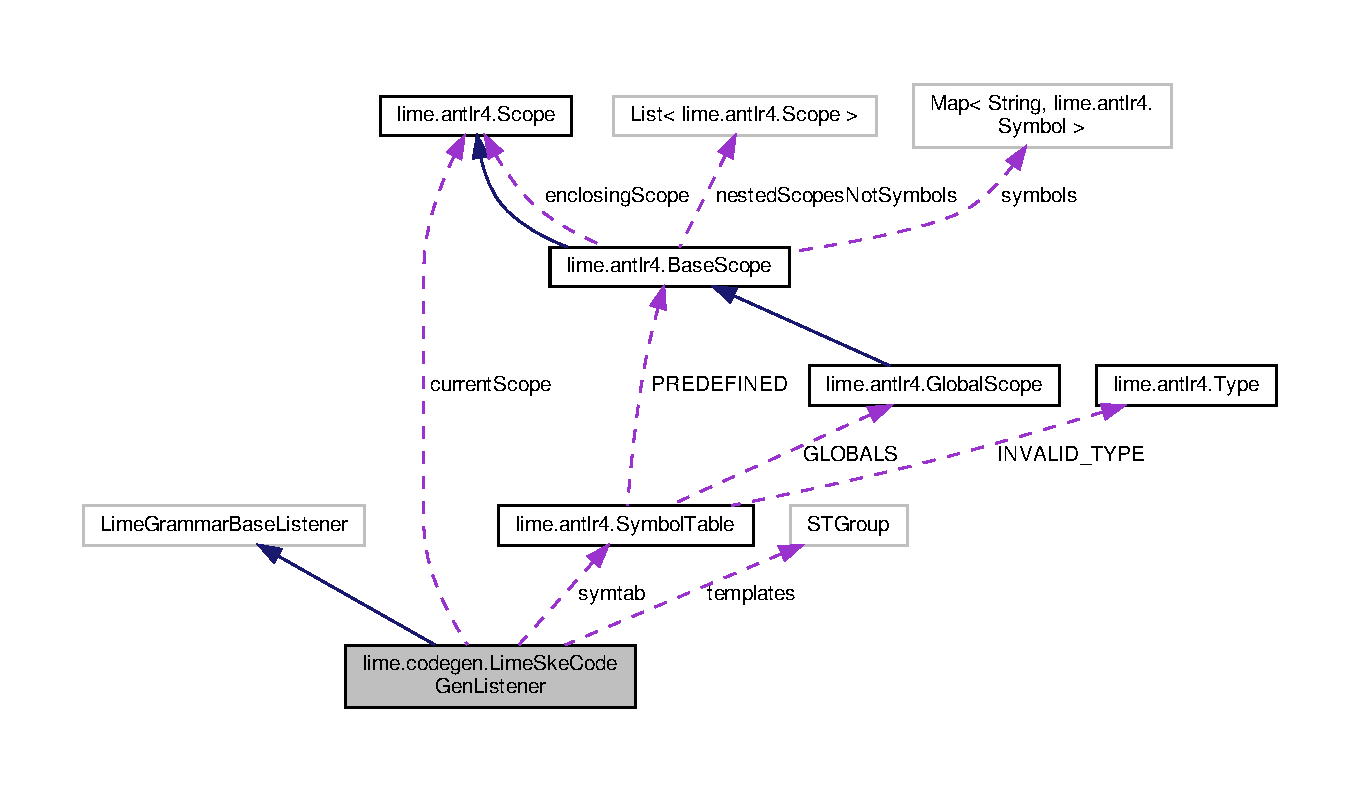
\includegraphics[width=350pt]{classlime_1_1codegen_1_1LimeSkeCodeGenListener__coll__graph}
\end{center}
\end{figure}
\subsection*{Public Member Functions}
\begin{DoxyCompactItemize}
\item 
\mbox{\Hypertarget{classlime_1_1codegen_1_1LimeSkeCodeGenListener_ab8f88655b019f6a4fe27f9d1f9075956}\label{classlime_1_1codegen_1_1LimeSkeCodeGenListener_ab8f88655b019f6a4fe27f9d1f9075956}} 
{\bfseries Lime\+Ske\+Code\+Gen\+Listener} (\hyperlink{classlime_1_1antlr4_1_1SymbolTable}{Symbol\+Table} st, S\+T\+Group stg)
\item 
\mbox{\Hypertarget{classlime_1_1codegen_1_1LimeSkeCodeGenListener_a63a8c969af0ab13db170745841d61ea6}\label{classlime_1_1codegen_1_1LimeSkeCodeGenListener_a63a8c969af0ab13db170745841d61ea6}} 
void {\bfseries enter\+Class\+Decl} (Class\+Decl\+Context ctx)
\item 
\mbox{\Hypertarget{classlime_1_1codegen_1_1LimeSkeCodeGenListener_a6af368640cf2e9bb3e6ce8e71ceb0d2f}\label{classlime_1_1codegen_1_1LimeSkeCodeGenListener_a6af368640cf2e9bb3e6ce8e71ceb0d2f}} 
void {\bfseries enter\+Action\+Decl} (Action\+Decl\+Context ctx)
\item 
\mbox{\Hypertarget{classlime_1_1codegen_1_1LimeSkeCodeGenListener_a1f8762af82b9637f34e07a4dd19d604a}\label{classlime_1_1codegen_1_1LimeSkeCodeGenListener_a1f8762af82b9637f34e07a4dd19d604a}} 
void {\bfseries enter\+Method\+Decl} (Method\+Decl\+Context ctx)
\item 
\mbox{\Hypertarget{classlime_1_1codegen_1_1LimeSkeCodeGenListener_a32015158a6d7849a051f67e38d34bd84}\label{classlime_1_1codegen_1_1LimeSkeCodeGenListener_a32015158a6d7849a051f67e38d34bd84}} 
void {\bfseries exit\+Class\+Decl} (Class\+Decl\+Context ctx)
\item 
\mbox{\Hypertarget{classlime_1_1codegen_1_1LimeSkeCodeGenListener_a2e8178e1a7aa817b968891b43536037d}\label{classlime_1_1codegen_1_1LimeSkeCodeGenListener_a2e8178e1a7aa817b968891b43536037d}} 
void {\bfseries exit\+Method\+Decl} (Method\+Decl\+Context ctx)
\item 
\mbox{\Hypertarget{classlime_1_1codegen_1_1LimeSkeCodeGenListener_a1801fffd10b9afb079ba3ba0208fd288}\label{classlime_1_1codegen_1_1LimeSkeCodeGenListener_a1801fffd10b9afb079ba3ba0208fd288}} 
void {\bfseries exit\+Action\+Decl} (Action\+Decl\+Context ctx)
\end{DoxyCompactItemize}


The documentation for this class was generated from the following file\+:\begin{DoxyCompactItemize}
\item 
src/lime/codegen/Lime\+Ske\+Code\+Gen\+Listener.\+java\end{DoxyCompactItemize}

\hypertarget{classlime_1_1antlr4_1_1LimeValue}{}\section{lime.\+antlr4.\+Lime\+Value Class Reference}
\label{classlime_1_1antlr4_1_1LimeValue}\index{lime.\+antlr4.\+Lime\+Value@{lime.\+antlr4.\+Lime\+Value}}


Inheritance diagram for lime.\+antlr4.\+Lime\+Value\+:
\nopagebreak
\begin{figure}[H]
\begin{center}
\leavevmode
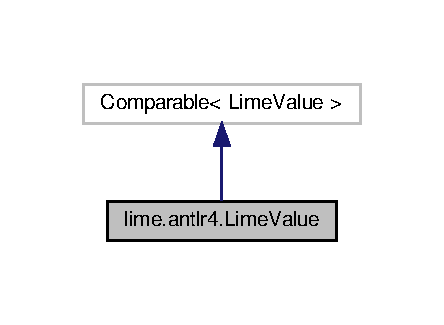
\includegraphics[width=213pt]{classlime_1_1antlr4_1_1LimeValue__inherit__graph}
\end{center}
\end{figure}


Collaboration diagram for lime.\+antlr4.\+Lime\+Value\+:
\nopagebreak
\begin{figure}[H]
\begin{center}
\leavevmode
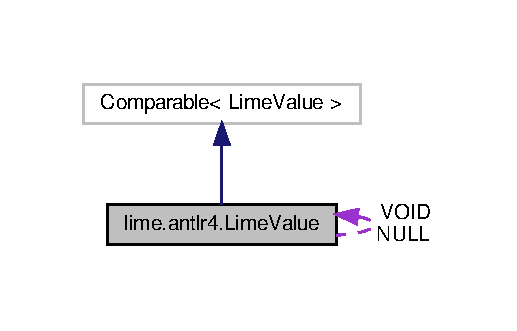
\includegraphics[width=248pt]{classlime_1_1antlr4_1_1LimeValue__coll__graph}
\end{center}
\end{figure}
\subsection*{Public Member Functions}
\begin{DoxyCompactItemize}
\item 
\mbox{\Hypertarget{classlime_1_1antlr4_1_1LimeValue_a443f1733e5b4063e559af82b64864c74}\label{classlime_1_1antlr4_1_1LimeValue_a443f1733e5b4063e559af82b64864c74}} 
int {\bfseries compare\+To} (\hyperlink{classlime_1_1antlr4_1_1LimeValue}{Lime\+Value} o)
\end{DoxyCompactItemize}
\subsection*{Static Public Attributes}
\begin{DoxyCompactItemize}
\item 
\mbox{\Hypertarget{classlime_1_1antlr4_1_1LimeValue_a153d87d8d830fece61c061abc25ddd4a}\label{classlime_1_1antlr4_1_1LimeValue_a153d87d8d830fece61c061abc25ddd4a}} 
static final \hyperlink{classlime_1_1antlr4_1_1LimeValue}{Lime\+Value} {\bfseries N\+U\+LL} = new \hyperlink{classlime_1_1antlr4_1_1LimeValue}{Lime\+Value}()
\item 
\mbox{\Hypertarget{classlime_1_1antlr4_1_1LimeValue_ae1b0cf57a5eb4493d3a0a82a4253829f}\label{classlime_1_1antlr4_1_1LimeValue_ae1b0cf57a5eb4493d3a0a82a4253829f}} 
static final \hyperlink{classlime_1_1antlr4_1_1LimeValue}{Lime\+Value} {\bfseries V\+O\+ID} = new \hyperlink{classlime_1_1antlr4_1_1LimeValue}{Lime\+Value}()
\end{DoxyCompactItemize}


The documentation for this class was generated from the following file\+:\begin{DoxyCompactItemize}
\item 
src/lime/antlr4/Lime\+Value.\+java\end{DoxyCompactItemize}

\hypertarget{classlime_1_1codegen_1_1LimeX86CodeGen}{}\section{lime.\+codegen.\+Lime\+X86\+Code\+Gen Class Reference}
\label{classlime_1_1codegen_1_1LimeX86CodeGen}\index{lime.\+codegen.\+Lime\+X86\+Code\+Gen@{lime.\+codegen.\+Lime\+X86\+Code\+Gen}}


The documentation for this class was generated from the following file\+:\begin{DoxyCompactItemize}
\item 
src/lime/codegen/Lime\+X86\+Code\+Gen.\+java\end{DoxyCompactItemize}

\hypertarget{classlime_1_1antlr4_1_1LocalScope}{}\section{lime.\+antlr4.\+Local\+Scope Class Reference}
\label{classlime_1_1antlr4_1_1LocalScope}\index{lime.\+antlr4.\+Local\+Scope@{lime.\+antlr4.\+Local\+Scope}}


Inheritance diagram for lime.\+antlr4.\+Local\+Scope\+:
\nopagebreak
\begin{figure}[H]
\begin{center}
\leavevmode
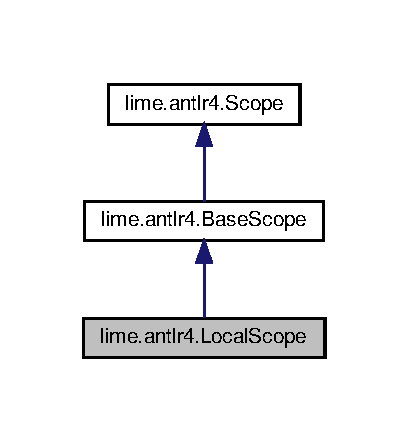
\includegraphics[width=196pt]{classlime_1_1antlr4_1_1LocalScope__inherit__graph}
\end{center}
\end{figure}


Collaboration diagram for lime.\+antlr4.\+Local\+Scope\+:
\nopagebreak
\begin{figure}[H]
\begin{center}
\leavevmode
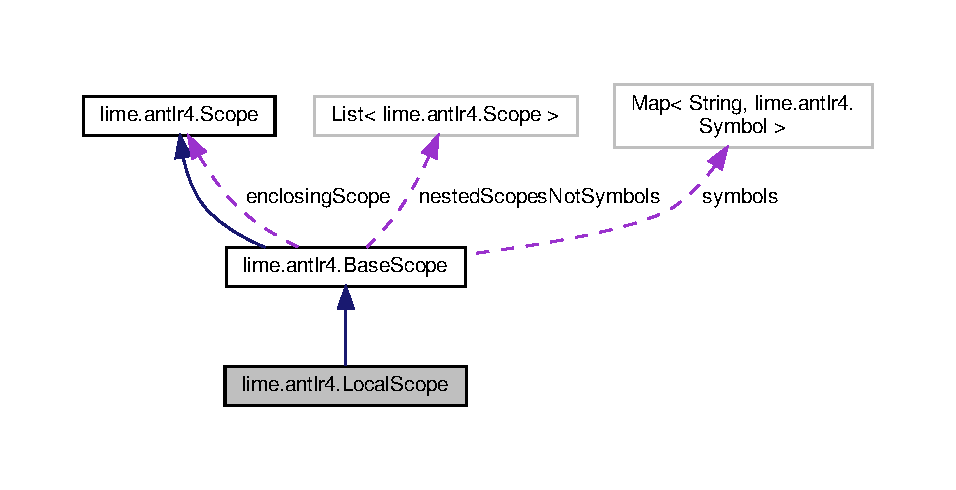
\includegraphics[width=350pt]{classlime_1_1antlr4_1_1LocalScope__coll__graph}
\end{center}
\end{figure}
\subsection*{Public Member Functions}
\begin{DoxyCompactItemize}
\item 
\mbox{\Hypertarget{classlime_1_1antlr4_1_1LocalScope_a99e6bbd9736491396241dbceed4a8a95}\label{classlime_1_1antlr4_1_1LocalScope_a99e6bbd9736491396241dbceed4a8a95}} 
{\bfseries Local\+Scope} (\hyperlink{interfacelime_1_1antlr4_1_1Scope}{Scope} enclosing\+Scope)
\item 
\mbox{\Hypertarget{classlime_1_1antlr4_1_1LocalScope_a503a34ad95208625ddbe8fda1473aa76}\label{classlime_1_1antlr4_1_1LocalScope_a503a34ad95208625ddbe8fda1473aa76}} 
String {\bfseries get\+Name} ()
\end{DoxyCompactItemize}
\subsection*{Additional Inherited Members}


The documentation for this class was generated from the following file\+:\begin{DoxyCompactItemize}
\item 
src/lime/antlr4/Local\+Scope.\+java\end{DoxyCompactItemize}

\hypertarget{classlime_1_1codegen_1_1Main}{}\section{lime.\+codegen.\+Main Class Reference}
\label{classlime_1_1codegen_1_1Main}\index{lime.\+codegen.\+Main@{lime.\+codegen.\+Main}}
\subsection*{Static Public Member Functions}
\begin{DoxyCompactItemize}
\item 
\mbox{\Hypertarget{classlime_1_1codegen_1_1Main_a7421c72e083e2b61d4a814c0c36fa7b2}\label{classlime_1_1codegen_1_1Main_a7421c72e083e2b61d4a814c0c36fa7b2}} 
static void {\bfseries main} (String\mbox{[}$\,$\mbox{]} args)
\item 
\mbox{\Hypertarget{classlime_1_1codegen_1_1Main_a34f35af613bde366a5efc1bf897fb441}\label{classlime_1_1codegen_1_1Main_a34f35af613bde366a5efc1bf897fb441}} 
static void {\bfseries parse} (File source)  throws Exception         
\item 
\mbox{\Hypertarget{classlime_1_1codegen_1_1Main_a51aa1aff40745622bddb428991e5cdec}\label{classlime_1_1codegen_1_1Main_a51aa1aff40745622bddb428991e5cdec}} 
static void {\bfseries build\+Json} (String source, \hyperlink{classlime_1_1antlr4_1_1SymbolTable}{Symbol\+Table} symtab, Map$<$ String, String $>$ guards)  throws Exception
\item 
\mbox{\Hypertarget{classlime_1_1codegen_1_1Main_ae1563b2445c300d15920f50364f2d363}\label{classlime_1_1codegen_1_1Main_ae1563b2445c300d15920f50364f2d363}} 
static void {\bfseries parse\+Source} (String source)  throws Exception         
\end{DoxyCompactItemize}


The documentation for this class was generated from the following file\+:\begin{DoxyCompactItemize}
\item 
src/lime/codegen/Main.\+java\end{DoxyCompactItemize}

\hypertarget{interfacelime_1_1antlr4_1_1MemberSymbol}{}\section{lime.\+antlr4.\+Member\+Symbol Interface Reference}
\label{interfacelime_1_1antlr4_1_1MemberSymbol}\index{lime.\+antlr4.\+Member\+Symbol@{lime.\+antlr4.\+Member\+Symbol}}


Inheritance diagram for lime.\+antlr4.\+Member\+Symbol\+:
\nopagebreak
\begin{figure}[H]
\begin{center}
\leavevmode
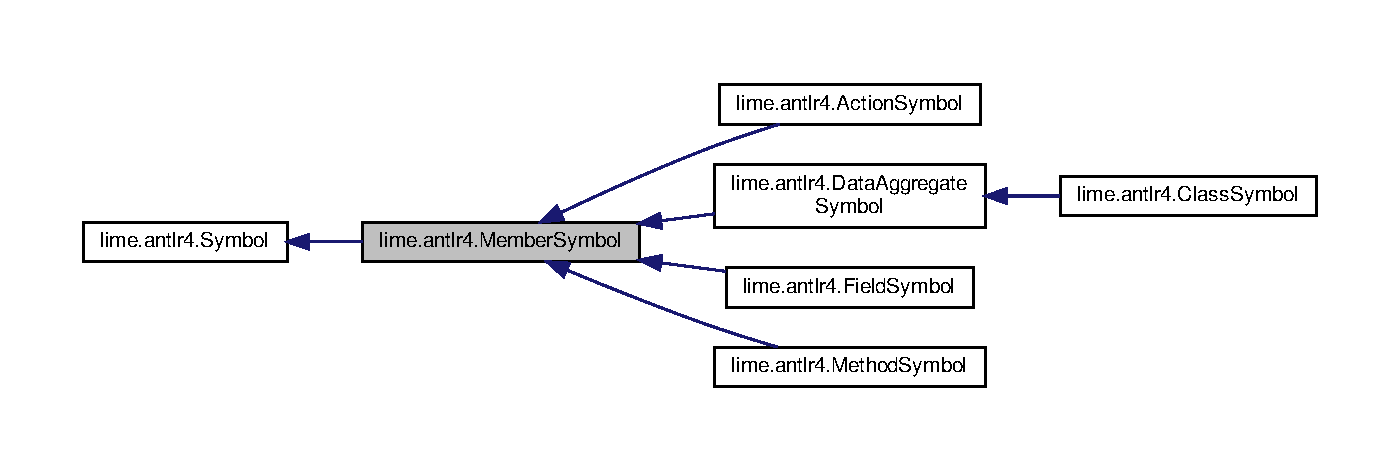
\includegraphics[width=350pt]{interfacelime_1_1antlr4_1_1MemberSymbol__inherit__graph}
\end{center}
\end{figure}


Collaboration diagram for lime.\+antlr4.\+Member\+Symbol\+:
\nopagebreak
\begin{figure}[H]
\begin{center}
\leavevmode
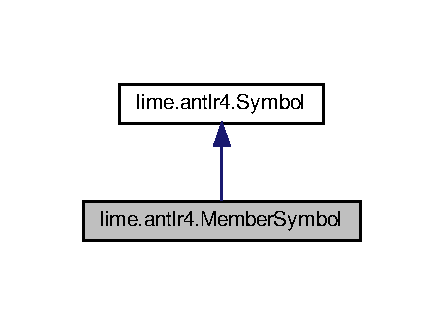
\includegraphics[width=213pt]{interfacelime_1_1antlr4_1_1MemberSymbol__coll__graph}
\end{center}
\end{figure}
\subsection*{Public Member Functions}
\begin{DoxyCompactItemize}
\item 
\mbox{\Hypertarget{interfacelime_1_1antlr4_1_1MemberSymbol_a0dd554e51511eed1a98745df9815eb40}\label{interfacelime_1_1antlr4_1_1MemberSymbol_a0dd554e51511eed1a98745df9815eb40}} 
int {\bfseries get\+Slot\+Number} ()
\end{DoxyCompactItemize}


The documentation for this interface was generated from the following file\+:\begin{DoxyCompactItemize}
\item 
src/lime/antlr4/Member\+Symbol.\+java\end{DoxyCompactItemize}

\hypertarget{classlime_1_1antlr4_1_1MethodSymbol}{}\section{lime.\+antlr4.\+Method\+Symbol Class Reference}
\label{classlime_1_1antlr4_1_1MethodSymbol}\index{lime.\+antlr4.\+Method\+Symbol@{lime.\+antlr4.\+Method\+Symbol}}


Inheritance diagram for lime.\+antlr4.\+Method\+Symbol\+:
\nopagebreak
\begin{figure}[H]
\begin{center}
\leavevmode
\includegraphics[width=350pt]{classlime_1_1antlr4_1_1MethodSymbol__inherit__graph}
\end{center}
\end{figure}


Collaboration diagram for lime.\+antlr4.\+Method\+Symbol\+:
\nopagebreak
\begin{figure}[H]
\begin{center}
\leavevmode
\includegraphics[width=350pt]{classlime_1_1antlr4_1_1MethodSymbol__coll__graph}
\end{center}
\end{figure}
\subsection*{Public Member Functions}
\begin{DoxyCompactItemize}
\item 
\mbox{\Hypertarget{classlime_1_1antlr4_1_1MethodSymbol_aef5560b833c2ba287a4b766de2a9ec62}\label{classlime_1_1antlr4_1_1MethodSymbol_aef5560b833c2ba287a4b766de2a9ec62}} 
{\bfseries Method\+Symbol} (String name)
\item 
\mbox{\Hypertarget{classlime_1_1antlr4_1_1MethodSymbol_ae2a590dd58724fc164ea49115989b15a}\label{classlime_1_1antlr4_1_1MethodSymbol_ae2a590dd58724fc164ea49115989b15a}} 
void {\bfseries set\+Enabled} (Set$<$ String $>$ cgids)
\item 
\mbox{\Hypertarget{classlime_1_1antlr4_1_1MethodSymbol_aa6379275becc3c4d8136b96be37a0f9d}\label{classlime_1_1antlr4_1_1MethodSymbol_aa6379275becc3c4d8136b96be37a0f9d}} 
int {\bfseries get\+Slot\+Number} ()
\item 
\mbox{\Hypertarget{classlime_1_1antlr4_1_1MethodSymbol_aaf32f229957e563ceeb098b8b7eb74be}\label{classlime_1_1antlr4_1_1MethodSymbol_aaf32f229957e563ceeb098b8b7eb74be}} 
boolean {\bfseries is\+Enabled} ()
\end{DoxyCompactItemize}
\subsection*{Public Attributes}
\begin{DoxyCompactItemize}
\item 
\mbox{\Hypertarget{classlime_1_1antlr4_1_1MethodSymbol_a4a763796e31c84ebbbbe3220697a33c4}\label{classlime_1_1antlr4_1_1MethodSymbol_a4a763796e31c84ebbbbe3220697a33c4}} 
Set$<$ String $>$ {\bfseries method\+Assign\+Lvalue}
\end{DoxyCompactItemize}
\subsection*{Protected Attributes}
\begin{DoxyCompactItemize}
\item 
\mbox{\Hypertarget{classlime_1_1antlr4_1_1MethodSymbol_af4bccbe42b535402c39faf9f1d68ae76}\label{classlime_1_1antlr4_1_1MethodSymbol_af4bccbe42b535402c39faf9f1d68ae76}} 
int {\bfseries slot} = -\/1
\item 
\mbox{\Hypertarget{classlime_1_1antlr4_1_1MethodSymbol_a316274a24ef39f41ea44c5f02c75032b}\label{classlime_1_1antlr4_1_1MethodSymbol_a316274a24ef39f41ea44c5f02c75032b}} 
boolean {\bfseries enabled} = false
\end{DoxyCompactItemize}


The documentation for this class was generated from the following file\+:\begin{DoxyCompactItemize}
\item 
src/lime/antlr4/Method\+Symbol.\+java\end{DoxyCompactItemize}

\hypertarget{classlime_1_1antlr4_1_1ParameterSymbol}{}\section{lime.\+antlr4.\+Parameter\+Symbol Class Reference}
\label{classlime_1_1antlr4_1_1ParameterSymbol}\index{lime.\+antlr4.\+Parameter\+Symbol@{lime.\+antlr4.\+Parameter\+Symbol}}


Inheritance diagram for lime.\+antlr4.\+Parameter\+Symbol\+:
\nopagebreak
\begin{figure}[H]
\begin{center}
\leavevmode
\includegraphics[width=344pt]{classlime_1_1antlr4_1_1ParameterSymbol__inherit__graph}
\end{center}
\end{figure}


Collaboration diagram for lime.\+antlr4.\+Parameter\+Symbol\+:
\nopagebreak
\begin{figure}[H]
\begin{center}
\leavevmode
\includegraphics[width=350pt]{classlime_1_1antlr4_1_1ParameterSymbol__coll__graph}
\end{center}
\end{figure}
\subsection*{Public Member Functions}
\begin{DoxyCompactItemize}
\item 
\mbox{\Hypertarget{classlime_1_1antlr4_1_1ParameterSymbol_aa8ec0fac38a490effa99255c9b778a19}\label{classlime_1_1antlr4_1_1ParameterSymbol_aa8ec0fac38a490effa99255c9b778a19}} 
{\bfseries Parameter\+Symbol} (String name)
\item 
\mbox{\Hypertarget{classlime_1_1antlr4_1_1ParameterSymbol_a4108c6c62a6011ca3def25251ab48cc9}\label{classlime_1_1antlr4_1_1ParameterSymbol_a4108c6c62a6011ca3def25251ab48cc9}} 
{\bfseries Parameter\+Symbol} (String name, int x)
\item 
\mbox{\Hypertarget{classlime_1_1antlr4_1_1ParameterSymbol_a57485eeee8a27fceec82e9aaa0a3b3ab}\label{classlime_1_1antlr4_1_1ParameterSymbol_a57485eeee8a27fceec82e9aaa0a3b3ab}} 
int {\bfseries get\+Index} ()
\end{DoxyCompactItemize}
\subsection*{Additional Inherited Members}


The documentation for this class was generated from the following file\+:\begin{DoxyCompactItemize}
\item 
src/lime/antlr4/Parameter\+Symbol.\+java\end{DoxyCompactItemize}

\hypertarget{classlime_1_1antlr4_1_1PointerType}{}\section{lime.\+antlr4.\+Pointer\+Type Class Reference}
\label{classlime_1_1antlr4_1_1PointerType}\index{lime.\+antlr4.\+Pointer\+Type@{lime.\+antlr4.\+Pointer\+Type}}


Inheritance diagram for lime.\+antlr4.\+Pointer\+Type\+:
\nopagebreak
\begin{figure}[H]
\begin{center}
\leavevmode
\includegraphics[width=197pt]{classlime_1_1antlr4_1_1PointerType__inherit__graph}
\end{center}
\end{figure}


Collaboration diagram for lime.\+antlr4.\+Pointer\+Type\+:
\nopagebreak
\begin{figure}[H]
\begin{center}
\leavevmode
\includegraphics[width=197pt]{classlime_1_1antlr4_1_1PointerType__coll__graph}
\end{center}
\end{figure}
\subsection*{Public Member Functions}
\begin{DoxyCompactItemize}
\item 
\mbox{\Hypertarget{classlime_1_1antlr4_1_1PointerType_a1cc426f8d589e506f4b4b23a20e96cf9}\label{classlime_1_1antlr4_1_1PointerType_a1cc426f8d589e506f4b4b23a20e96cf9}} 
{\bfseries Pointer\+Type} (\hyperlink{interfacelime_1_1antlr4_1_1Type}{Type} target\+Type)
\item 
\mbox{\Hypertarget{classlime_1_1antlr4_1_1PointerType_ad3473dffd49cc3270fbf81d752949647}\label{classlime_1_1antlr4_1_1PointerType_ad3473dffd49cc3270fbf81d752949647}} 
String {\bfseries get\+Name} ()
\item 
\mbox{\Hypertarget{classlime_1_1antlr4_1_1PointerType_a5cea4480b1ed7e29003304d8f5be87a0}\label{classlime_1_1antlr4_1_1PointerType_a5cea4480b1ed7e29003304d8f5be87a0}} 
int {\bfseries get\+Type\+Index} ()
\item 
\mbox{\Hypertarget{classlime_1_1antlr4_1_1PointerType_aaee793b566aa57a5f96f18db0c8d73a0}\label{classlime_1_1antlr4_1_1PointerType_aaee793b566aa57a5f96f18db0c8d73a0}} 
String {\bfseries to\+String} ()
\end{DoxyCompactItemize}
\subsection*{Protected Attributes}
\begin{DoxyCompactItemize}
\item 
\mbox{\Hypertarget{classlime_1_1antlr4_1_1PointerType_a5f043fdd0c4e4eea5880a754abda958c}\label{classlime_1_1antlr4_1_1PointerType_a5f043fdd0c4e4eea5880a754abda958c}} 
\hyperlink{interfacelime_1_1antlr4_1_1Type}{Type} {\bfseries target\+Type}
\end{DoxyCompactItemize}


The documentation for this class was generated from the following file\+:\begin{DoxyCompactItemize}
\item 
src/lime/antlr4/Pointer\+Type.\+java\end{DoxyCompactItemize}

\hypertarget{classlime_1_1antlr4_1_1PredefinedScope}{}\section{lime.\+antlr4.\+Predefined\+Scope Class Reference}
\label{classlime_1_1antlr4_1_1PredefinedScope}\index{lime.\+antlr4.\+Predefined\+Scope@{lime.\+antlr4.\+Predefined\+Scope}}


Inheritance diagram for lime.\+antlr4.\+Predefined\+Scope\+:
\nopagebreak
\begin{figure}[H]
\begin{center}
\leavevmode
\includegraphics[width=219pt]{classlime_1_1antlr4_1_1PredefinedScope__inherit__graph}
\end{center}
\end{figure}


Collaboration diagram for lime.\+antlr4.\+Predefined\+Scope\+:
\nopagebreak
\begin{figure}[H]
\begin{center}
\leavevmode
\includegraphics[width=350pt]{classlime_1_1antlr4_1_1PredefinedScope__coll__graph}
\end{center}
\end{figure}
\subsection*{Public Member Functions}
\begin{DoxyCompactItemize}
\item 
\mbox{\Hypertarget{classlime_1_1antlr4_1_1PredefinedScope_ac57f825f765c97a510da7512f5760266}\label{classlime_1_1antlr4_1_1PredefinedScope_ac57f825f765c97a510da7512f5760266}} 
String {\bfseries get\+Name} ()
\end{DoxyCompactItemize}
\subsection*{Additional Inherited Members}


The documentation for this class was generated from the following file\+:\begin{DoxyCompactItemize}
\item 
src/lime/antlr4/Predefined\+Scope.\+java\end{DoxyCompactItemize}

\hypertarget{classlime_1_1antlr4_1_1PrimitiveType}{}\section{lime.\+antlr4.\+Primitive\+Type Class Reference}
\label{classlime_1_1antlr4_1_1PrimitiveType}\index{lime.\+antlr4.\+Primitive\+Type@{lime.\+antlr4.\+Primitive\+Type}}


Inheritance diagram for lime.\+antlr4.\+Primitive\+Type\+:
\nopagebreak
\begin{figure}[H]
\begin{center}
\leavevmode
\includegraphics[width=304pt]{classlime_1_1antlr4_1_1PrimitiveType__inherit__graph}
\end{center}
\end{figure}


Collaboration diagram for lime.\+antlr4.\+Primitive\+Type\+:
\nopagebreak
\begin{figure}[H]
\begin{center}
\leavevmode
\includegraphics[width=350pt]{classlime_1_1antlr4_1_1PrimitiveType__coll__graph}
\end{center}
\end{figure}
\subsection*{Public Member Functions}
\begin{DoxyCompactItemize}
\item 
\mbox{\Hypertarget{classlime_1_1antlr4_1_1PrimitiveType_aee03611ee38ae98eb5b7399a66c2c45f}\label{classlime_1_1antlr4_1_1PrimitiveType_aee03611ee38ae98eb5b7399a66c2c45f}} 
{\bfseries Primitive\+Type} (String name)
\item 
\mbox{\Hypertarget{classlime_1_1antlr4_1_1PrimitiveType_af9a41e3f2334f1351767ad7a9cd5a13b}\label{classlime_1_1antlr4_1_1PrimitiveType_af9a41e3f2334f1351767ad7a9cd5a13b}} 
int {\bfseries get\+Type\+Index} ()
\item 
\mbox{\Hypertarget{classlime_1_1antlr4_1_1PrimitiveType_a9b2a3b3ef9d73c1dec2d19c3dfe922b4}\label{classlime_1_1antlr4_1_1PrimitiveType_a9b2a3b3ef9d73c1dec2d19c3dfe922b4}} 
void {\bfseries set\+Type\+Index} (int type\+Index)
\item 
\mbox{\Hypertarget{classlime_1_1antlr4_1_1PrimitiveType_a0ed087b1514f4926ee1b2c8e6b98be7d}\label{classlime_1_1antlr4_1_1PrimitiveType_a0ed087b1514f4926ee1b2c8e6b98be7d}} 
String {\bfseries get\+Name} ()
\end{DoxyCompactItemize}
\subsection*{Protected Attributes}
\begin{DoxyCompactItemize}
\item 
\mbox{\Hypertarget{classlime_1_1antlr4_1_1PrimitiveType_a78bcb81ffb77ba561fd312bc9a80bc01}\label{classlime_1_1antlr4_1_1PrimitiveType_a78bcb81ffb77ba561fd312bc9a80bc01}} 
int {\bfseries type\+Index}
\end{DoxyCompactItemize}


The documentation for this class was generated from the following file\+:\begin{DoxyCompactItemize}
\item 
src/lime/antlr4/Primitive\+Type.\+java\end{DoxyCompactItemize}

\hypertarget{classlime_1_1backend_1_1Register}{}\section{lime.\+backend.\+Register Class Reference}
\label{classlime_1_1backend_1_1Register}\index{lime.\+backend.\+Register@{lime.\+backend.\+Register}}


Inheritance diagram for lime.\+backend.\+Register\+:
\nopagebreak
\begin{figure}[H]
\begin{center}
\leavevmode
\includegraphics[width=247pt]{classlime_1_1backend_1_1Register__inherit__graph}
\end{center}
\end{figure}


Collaboration diagram for lime.\+backend.\+Register\+:
\nopagebreak
\begin{figure}[H]
\begin{center}
\leavevmode
\includegraphics[width=194pt]{classlime_1_1backend_1_1Register__coll__graph}
\end{center}
\end{figure}
\subsection*{Public Member Functions}
\begin{DoxyCompactItemize}
\item 
\mbox{\Hypertarget{classlime_1_1backend_1_1Register_a9664f3d28d224d923764d249d069d297}\label{classlime_1_1backend_1_1Register_a9664f3d28d224d923764d249d069d297}} 
{\bfseries Register} (String str)
\item 
\mbox{\Hypertarget{classlime_1_1backend_1_1Register_a7c04fe0eddd1dc4fee79868333a9771d}\label{classlime_1_1backend_1_1Register_a7c04fe0eddd1dc4fee79868333a9771d}} 
{\bfseries Register} (\hyperlink{classlime_1_1backend_1_1Register}{Register} register)
\item 
\mbox{\Hypertarget{classlime_1_1backend_1_1Register_a7230122f9f91c7f26ccc306d9ce46f8f}\label{classlime_1_1backend_1_1Register_a7230122f9f91c7f26ccc306d9ce46f8f}} 
String {\bfseries to\+String} ()
\end{DoxyCompactItemize}
\subsection*{Additional Inherited Members}


The documentation for this class was generated from the following file\+:\begin{DoxyCompactItemize}
\item 
src/lime/backend/Register.\+java\end{DoxyCompactItemize}

\hypertarget{classlime_1_1backend_1_1RegisterDereference}{}\section{lime.\+backend.\+Register\+Dereference Class Reference}
\label{classlime_1_1backend_1_1RegisterDereference}\index{lime.\+backend.\+Register\+Dereference@{lime.\+backend.\+Register\+Dereference}}


Inheritance diagram for lime.\+backend.\+Register\+Dereference\+:
\nopagebreak
\begin{figure}[H]
\begin{center}
\leavevmode
\includegraphics[width=247pt]{classlime_1_1backend_1_1RegisterDereference__inherit__graph}
\end{center}
\end{figure}


Collaboration diagram for lime.\+backend.\+Register\+Dereference\+:
\nopagebreak
\begin{figure}[H]
\begin{center}
\leavevmode
\includegraphics[width=247pt]{classlime_1_1backend_1_1RegisterDereference__coll__graph}
\end{center}
\end{figure}
\subsection*{Public Member Functions}
\begin{DoxyCompactItemize}
\item 
\mbox{\Hypertarget{classlime_1_1backend_1_1RegisterDereference_a0cd39b3f415b747472fd456751186624}\label{classlime_1_1backend_1_1RegisterDereference_a0cd39b3f415b747472fd456751186624}} 
{\bfseries Register\+Dereference} (String str)
\item 
\mbox{\Hypertarget{classlime_1_1backend_1_1RegisterDereference_a9ecdc687544a8c54aaa4e4cb8c2ce7ce}\label{classlime_1_1backend_1_1RegisterDereference_a9ecdc687544a8c54aaa4e4cb8c2ce7ce}} 
String {\bfseries to\+String} ()
\end{DoxyCompactItemize}
\subsection*{Additional Inherited Members}


The documentation for this class was generated from the following file\+:\begin{DoxyCompactItemize}
\item 
src/lime/backend/Register\+Dereference.\+java\end{DoxyCompactItemize}

\hypertarget{interfacelime_1_1backend_1_1RegisterManager}{}\section{lime.\+backend.\+Register\+Manager Interface Reference}
\label{interfacelime_1_1backend_1_1RegisterManager}\index{lime.\+backend.\+Register\+Manager@{lime.\+backend.\+Register\+Manager}}


Inheritance diagram for lime.\+backend.\+Register\+Manager\+:
\nopagebreak
\begin{figure}[H]
\begin{center}
\leavevmode
\includegraphics[width=232pt]{interfacelime_1_1backend_1_1RegisterManager__inherit__graph}
\end{center}
\end{figure}
\subsection*{Public Member Functions}
\begin{DoxyCompactItemize}
\item 
\mbox{\Hypertarget{interfacelime_1_1backend_1_1RegisterManager_a4bae4a1dd4c13e2d86ab07c78c7cbddd}\label{interfacelime_1_1backend_1_1RegisterManager_a4bae4a1dd4c13e2d86ab07c78c7cbddd}} 
\hyperlink{classlime_1_1backend_1_1Register}{Register} {\bfseries get\+Register\+By\+Index} (int i)
\end{DoxyCompactItemize}


The documentation for this interface was generated from the following file\+:\begin{DoxyCompactItemize}
\item 
src/lime/backend/Register\+Manager.\+java\end{DoxyCompactItemize}

\hypertarget{interfacelime_1_1antlr4_1_1Scope}{}\section{lime.\+antlr4.\+Scope Interface Reference}
\label{interfacelime_1_1antlr4_1_1Scope}\index{lime.\+antlr4.\+Scope@{lime.\+antlr4.\+Scope}}


Inheritance diagram for lime.\+antlr4.\+Scope\+:
\nopagebreak
\begin{figure}[H]
\begin{center}
\leavevmode
\includegraphics[width=350pt]{interfacelime_1_1antlr4_1_1Scope__inherit__graph}
\end{center}
\end{figure}
\subsection*{Public Member Functions}
\begin{DoxyCompactItemize}
\item 
\mbox{\Hypertarget{interfacelime_1_1antlr4_1_1Scope_aef43f9cd973a1a31c005c8fe44db65a0}\label{interfacelime_1_1antlr4_1_1Scope_aef43f9cd973a1a31c005c8fe44db65a0}} 
String {\bfseries get\+Name} ()
\item 
\mbox{\Hypertarget{interfacelime_1_1antlr4_1_1Scope_a7fb3b80a70c0c0828bbd5539851207b9}\label{interfacelime_1_1antlr4_1_1Scope_a7fb3b80a70c0c0828bbd5539851207b9}} 
\hyperlink{interfacelime_1_1antlr4_1_1Scope}{Scope} {\bfseries get\+Enclosing\+Scope} ()
\item 
\mbox{\Hypertarget{interfacelime_1_1antlr4_1_1Scope_a55166ac3b34d96eb8880a99e6a6b103e}\label{interfacelime_1_1antlr4_1_1Scope_a55166ac3b34d96eb8880a99e6a6b103e}} 
void {\bfseries set\+Enclosing\+Scope} (\hyperlink{interfacelime_1_1antlr4_1_1Scope}{Scope} s)
\item 
\mbox{\Hypertarget{interfacelime_1_1antlr4_1_1Scope_ae00121132c58b59c9068ce8fdbfda038}\label{interfacelime_1_1antlr4_1_1Scope_ae00121132c58b59c9068ce8fdbfda038}} 
void {\bfseries define} (\hyperlink{interfacelime_1_1antlr4_1_1Symbol}{Symbol} sym)  throws Illegal\+Argument\+Exception
\item 
\mbox{\Hypertarget{interfacelime_1_1antlr4_1_1Scope_a2e47a3f05a1ebee278deef9b04ee5329}\label{interfacelime_1_1antlr4_1_1Scope_a2e47a3f05a1ebee278deef9b04ee5329}} 
\hyperlink{interfacelime_1_1antlr4_1_1Symbol}{Symbol} {\bfseries resolve} (String name)
\item 
\mbox{\Hypertarget{interfacelime_1_1antlr4_1_1Scope_ae5aee3e1d939631a9c3ea7dcd02410cb}\label{interfacelime_1_1antlr4_1_1Scope_ae5aee3e1d939631a9c3ea7dcd02410cb}} 
\hyperlink{interfacelime_1_1antlr4_1_1Symbol}{Symbol} {\bfseries get\+Symbol} (String name)
\item 
\mbox{\Hypertarget{interfacelime_1_1antlr4_1_1Scope_a2db507561bb359243c05663b7eb43c3f}\label{interfacelime_1_1antlr4_1_1Scope_a2db507561bb359243c05663b7eb43c3f}} 
void {\bfseries nest} (\hyperlink{interfacelime_1_1antlr4_1_1Scope}{Scope} scope)  throws Illegal\+Argument\+Exception
\item 
\mbox{\Hypertarget{interfacelime_1_1antlr4_1_1Scope_a9a20c558459e662c9f9c112b58d6db47}\label{interfacelime_1_1antlr4_1_1Scope_a9a20c558459e662c9f9c112b58d6db47}} 
List$<$ \hyperlink{interfacelime_1_1antlr4_1_1Scope}{Scope} $>$ {\bfseries get\+Nested\+Scopes} ()
\item 
\mbox{\Hypertarget{interfacelime_1_1antlr4_1_1Scope_ae8867ed33fcb9f328c7ee750c4202886}\label{interfacelime_1_1antlr4_1_1Scope_ae8867ed33fcb9f328c7ee750c4202886}} 
List$<$ \hyperlink{interfacelime_1_1antlr4_1_1Scope}{Scope} $>$ {\bfseries get\+Enclosing\+Path\+To\+Root} ()
\item 
\mbox{\Hypertarget{interfacelime_1_1antlr4_1_1Scope_afdea18675031436423be0e76369c732b}\label{interfacelime_1_1antlr4_1_1Scope_afdea18675031436423be0e76369c732b}} 
List$<$ \hyperlink{interfacelime_1_1antlr4_1_1Scope}{Scope} $>$ {\bfseries get\+Nested\+Scoped\+Symbols} ()
\item 
\mbox{\Hypertarget{interfacelime_1_1antlr4_1_1Scope_ad873f9629210aed09d2c02651d363e49}\label{interfacelime_1_1antlr4_1_1Scope_ad873f9629210aed09d2c02651d363e49}} 
List$<$? extends \hyperlink{interfacelime_1_1antlr4_1_1Symbol}{Symbol} $>$ {\bfseries get\+Symbols} ()
\item 
\mbox{\Hypertarget{interfacelime_1_1antlr4_1_1Scope_aeb4969f6d0b9e4caadbe70c7aa9d398b}\label{interfacelime_1_1antlr4_1_1Scope_aeb4969f6d0b9e4caadbe70c7aa9d398b}} 
List$<$? extends \hyperlink{interfacelime_1_1antlr4_1_1Symbol}{Symbol} $>$ {\bfseries get\+All\+Symbols} ()
\item 
\mbox{\Hypertarget{interfacelime_1_1antlr4_1_1Scope_a82efdd706f75c5192a88213a5dab8701}\label{interfacelime_1_1antlr4_1_1Scope_a82efdd706f75c5192a88213a5dab8701}} 
Set$<$ String $>$ {\bfseries get\+Symbol\+Names} ()
\item 
\mbox{\Hypertarget{interfacelime_1_1antlr4_1_1Scope_a6f4548cd09e74a74b532c127c16f0661}\label{interfacelime_1_1antlr4_1_1Scope_a6f4548cd09e74a74b532c127c16f0661}} 
int {\bfseries get\+Number\+Of\+Symbols} ()
\item 
\mbox{\Hypertarget{interfacelime_1_1antlr4_1_1Scope_a91aefa36f23823d60d968ef9bede6b11}\label{interfacelime_1_1antlr4_1_1Scope_a91aefa36f23823d60d968ef9bede6b11}} 
String {\bfseries to\+Qualifier\+String} (String separator)
\end{DoxyCompactItemize}


The documentation for this interface was generated from the following file\+:\begin{DoxyCompactItemize}
\item 
src/lime/antlr4/Scope.\+java\end{DoxyCompactItemize}

\hypertarget{classlime_1_1backend_1_1StackOffset}{}\section{lime.\+backend.\+Stack\+Offset Class Reference}
\label{classlime_1_1backend_1_1StackOffset}\index{lime.\+backend.\+Stack\+Offset@{lime.\+backend.\+Stack\+Offset}}


Inheritance diagram for lime.\+backend.\+Stack\+Offset\+:
\nopagebreak
\begin{figure}[H]
\begin{center}
\leavevmode
\includegraphics[width=210pt]{classlime_1_1backend_1_1StackOffset__inherit__graph}
\end{center}
\end{figure}


Collaboration diagram for lime.\+backend.\+Stack\+Offset\+:
\nopagebreak
\begin{figure}[H]
\begin{center}
\leavevmode
\includegraphics[width=210pt]{classlime_1_1backend_1_1StackOffset__coll__graph}
\end{center}
\end{figure}
\subsection*{Public Member Functions}
\begin{DoxyCompactItemize}
\item 
\mbox{\Hypertarget{classlime_1_1backend_1_1StackOffset_a9d764ed11b28e716f5a4427c8a3f9386}\label{classlime_1_1backend_1_1StackOffset_a9d764ed11b28e716f5a4427c8a3f9386}} 
{\bfseries Stack\+Offset} (String str)
\item 
\mbox{\Hypertarget{classlime_1_1backend_1_1StackOffset_a6b198f2856ca626618b83f70220af5e1}\label{classlime_1_1backend_1_1StackOffset_a6b198f2856ca626618b83f70220af5e1}} 
String {\bfseries to\+String} ()
\end{DoxyCompactItemize}
\subsection*{Additional Inherited Members}


The documentation for this class was generated from the following file\+:\begin{DoxyCompactItemize}
\item 
src/lime/backend/Stack\+Offset.\+java\end{DoxyCompactItemize}

\hypertarget{interfacelime_1_1antlr4_1_1Symbol}{}\section{lime.\+antlr4.\+Symbol Interface Reference}
\label{interfacelime_1_1antlr4_1_1Symbol}\index{lime.\+antlr4.\+Symbol@{lime.\+antlr4.\+Symbol}}


Inheritance diagram for lime.\+antlr4.\+Symbol\+:
\nopagebreak
\begin{figure}[H]
\begin{center}
\leavevmode
\includegraphics[width=350pt]{interfacelime_1_1antlr4_1_1Symbol__inherit__graph}
\end{center}
\end{figure}
\subsection*{Public Member Functions}
\begin{DoxyCompactItemize}
\item 
\mbox{\Hypertarget{interfacelime_1_1antlr4_1_1Symbol_a505dfda70e62ed930ddc16eba30014ca}\label{interfacelime_1_1antlr4_1_1Symbol_a505dfda70e62ed930ddc16eba30014ca}} 
String {\bfseries get\+Name} ()
\item 
\mbox{\Hypertarget{interfacelime_1_1antlr4_1_1Symbol_a0628643d2a4ad033592e6f92f1941db8}\label{interfacelime_1_1antlr4_1_1Symbol_a0628643d2a4ad033592e6f92f1941db8}} 
\hyperlink{interfacelime_1_1antlr4_1_1Scope}{Scope} {\bfseries get\+Scope} ()
\item 
\mbox{\Hypertarget{interfacelime_1_1antlr4_1_1Symbol_ab3cf8527aee569afe5b6ae0d82d50571}\label{interfacelime_1_1antlr4_1_1Symbol_ab3cf8527aee569afe5b6ae0d82d50571}} 
void {\bfseries set\+Scope} (\hyperlink{interfacelime_1_1antlr4_1_1Scope}{Scope} scope)
\item 
\mbox{\Hypertarget{interfacelime_1_1antlr4_1_1Symbol_a6b92e91502cec05cc20a3c5e24a65149}\label{interfacelime_1_1antlr4_1_1Symbol_a6b92e91502cec05cc20a3c5e24a65149}} 
int {\bfseries get\+Insertion\+Order\+Number} ()
\item 
\mbox{\Hypertarget{interfacelime_1_1antlr4_1_1Symbol_a3ce1633e8c869671a7e835709717cb74}\label{interfacelime_1_1antlr4_1_1Symbol_a3ce1633e8c869671a7e835709717cb74}} 
void {\bfseries set\+Insertion\+Order\+Number} (int i)
\item 
\mbox{\Hypertarget{interfacelime_1_1antlr4_1_1Symbol_a1530de334023c9d0138eae63fb4928df}\label{interfacelime_1_1antlr4_1_1Symbol_a1530de334023c9d0138eae63fb4928df}} 
int {\bfseries hash\+Code} ()
\item 
\mbox{\Hypertarget{interfacelime_1_1antlr4_1_1Symbol_a830fa4adfbb899a00613ba8e29588278}\label{interfacelime_1_1antlr4_1_1Symbol_a830fa4adfbb899a00613ba8e29588278}} 
boolean {\bfseries equals} (Object o)
\end{DoxyCompactItemize}


The documentation for this interface was generated from the following file\+:\begin{DoxyCompactItemize}
\item 
src/lime/antlr4/Symbol.\+java\end{DoxyCompactItemize}

\hypertarget{classlime_1_1antlr4_1_1SymbolTable}{}\section{lime.\+antlr4.\+Symbol\+Table Class Reference}
\label{classlime_1_1antlr4_1_1SymbolTable}\index{lime.\+antlr4.\+Symbol\+Table@{lime.\+antlr4.\+Symbol\+Table}}


Collaboration diagram for lime.\+antlr4.\+Symbol\+Table\+:
\nopagebreak
\begin{figure}[H]
\begin{center}
\leavevmode
\includegraphics[width=350pt]{classlime_1_1antlr4_1_1SymbolTable__coll__graph}
\end{center}
\end{figure}
\subsection*{Public Member Functions}
\begin{DoxyCompactItemize}
\item 
\mbox{\Hypertarget{classlime_1_1antlr4_1_1SymbolTable_a27f190e7d7fe7cf06200de4c74b2c639}\label{classlime_1_1antlr4_1_1SymbolTable_a27f190e7d7fe7cf06200de4c74b2c639}} 
void {\bfseries init\+Type\+System} ()
\item 
\mbox{\Hypertarget{classlime_1_1antlr4_1_1SymbolTable_a9af67845f1fe3396ed6d357afa5c492e}\label{classlime_1_1antlr4_1_1SymbolTable_a9af67845f1fe3396ed6d357afa5c492e}} 
void {\bfseries define\+Predefined\+Symbol} (\hyperlink{interfacelime_1_1antlr4_1_1Symbol}{Symbol} s)
\item 
\mbox{\Hypertarget{classlime_1_1antlr4_1_1SymbolTable_a45cc089feae931761e21573b2552fc0c}\label{classlime_1_1antlr4_1_1SymbolTable_a45cc089feae931761e21573b2552fc0c}} 
void {\bfseries define\+Global\+Symbol} (\hyperlink{interfacelime_1_1antlr4_1_1Symbol}{Symbol} s)
\end{DoxyCompactItemize}
\subsection*{Public Attributes}
\begin{DoxyCompactItemize}
\item 
\mbox{\Hypertarget{classlime_1_1antlr4_1_1SymbolTable_a7ded93f922e3305d0e1c20deefc0cb79}\label{classlime_1_1antlr4_1_1SymbolTable_a7ded93f922e3305d0e1c20deefc0cb79}} 
\hyperlink{classlime_1_1antlr4_1_1BaseScope}{Base\+Scope} {\bfseries P\+R\+E\+D\+E\+F\+I\+N\+ED} = new \hyperlink{classlime_1_1antlr4_1_1PredefinedScope}{Predefined\+Scope}()
\item 
\mbox{\Hypertarget{classlime_1_1antlr4_1_1SymbolTable_a02a3f5f95d5cbd6d489d8c6fa5eb3da6}\label{classlime_1_1antlr4_1_1SymbolTable_a02a3f5f95d5cbd6d489d8c6fa5eb3da6}} 
\hyperlink{classlime_1_1antlr4_1_1GlobalScope}{Global\+Scope} {\bfseries G\+L\+O\+B\+A\+LS} = new \hyperlink{classlime_1_1antlr4_1_1GlobalScope}{Global\+Scope}(P\+R\+E\+D\+E\+F\+I\+N\+ED)
\end{DoxyCompactItemize}
\subsection*{Static Public Attributes}
\begin{DoxyCompactItemize}
\item 
\mbox{\Hypertarget{classlime_1_1antlr4_1_1SymbolTable_aabd5311e02b31576a44c94070a480108}\label{classlime_1_1antlr4_1_1SymbolTable_aabd5311e02b31576a44c94070a480108}} 
static final \hyperlink{interfacelime_1_1antlr4_1_1Type}{Type} {\bfseries I\+N\+V\+A\+L\+I\+D\+\_\+\+T\+Y\+PE} = new \hyperlink{classlime_1_1antlr4_1_1InvalidType}{Invalid\+Type}()
\end{DoxyCompactItemize}


The documentation for this class was generated from the following file\+:\begin{DoxyCompactItemize}
\item 
src/lime/antlr4/Symbol\+Table.\+java\end{DoxyCompactItemize}

\hypertarget{classlime_1_1antlr4_1_1SymbolWithScope}{}\section{lime.\+antlr4.\+Symbol\+With\+Scope Class Reference}
\label{classlime_1_1antlr4_1_1SymbolWithScope}\index{lime.\+antlr4.\+Symbol\+With\+Scope@{lime.\+antlr4.\+Symbol\+With\+Scope}}


Inheritance diagram for lime.\+antlr4.\+Symbol\+With\+Scope\+:
\nopagebreak
\begin{figure}[H]
\begin{center}
\leavevmode
\includegraphics[width=350pt]{classlime_1_1antlr4_1_1SymbolWithScope__inherit__graph}
\end{center}
\end{figure}


Collaboration diagram for lime.\+antlr4.\+Symbol\+With\+Scope\+:
\nopagebreak
\begin{figure}[H]
\begin{center}
\leavevmode
\includegraphics[width=350pt]{classlime_1_1antlr4_1_1SymbolWithScope__coll__graph}
\end{center}
\end{figure}
\subsection*{Public Member Functions}
\begin{DoxyCompactItemize}
\item 
\mbox{\Hypertarget{classlime_1_1antlr4_1_1SymbolWithScope_a3c505ddb292cf2d4166938e06f96c427}\label{classlime_1_1antlr4_1_1SymbolWithScope_a3c505ddb292cf2d4166938e06f96c427}} 
{\bfseries Symbol\+With\+Scope} (String name)
\item 
\mbox{\Hypertarget{classlime_1_1antlr4_1_1SymbolWithScope_aac22203297178d4b686062f3ed080f2a}\label{classlime_1_1antlr4_1_1SymbolWithScope_aac22203297178d4b686062f3ed080f2a}} 
String {\bfseries get\+Name} ()
\item 
\mbox{\Hypertarget{classlime_1_1antlr4_1_1SymbolWithScope_a53bfb3b22d84aa9bd870665af4b6c90c}\label{classlime_1_1antlr4_1_1SymbolWithScope_a53bfb3b22d84aa9bd870665af4b6c90c}} 
\hyperlink{interfacelime_1_1antlr4_1_1Scope}{Scope} {\bfseries get\+Scope} ()
\item 
\mbox{\Hypertarget{classlime_1_1antlr4_1_1SymbolWithScope_a6a08ad294932ce212aa339bd3ce4b997}\label{classlime_1_1antlr4_1_1SymbolWithScope_a6a08ad294932ce212aa339bd3ce4b997}} 
void {\bfseries set\+Scope} (\hyperlink{interfacelime_1_1antlr4_1_1Scope}{Scope} scope)
\item 
\mbox{\Hypertarget{classlime_1_1antlr4_1_1SymbolWithScope_a4488146ee888a010983dfccf8b368b20}\label{classlime_1_1antlr4_1_1SymbolWithScope_a4488146ee888a010983dfccf8b368b20}} 
\hyperlink{interfacelime_1_1antlr4_1_1Scope}{Scope} {\bfseries get\+Enclosing\+Scope} ()
\item 
String \hyperlink{classlime_1_1antlr4_1_1SymbolWithScope_a84495a0d09bc077969de2108fab615c1}{get\+Qualified\+Name} ()
\item 
String \hyperlink{classlime_1_1antlr4_1_1SymbolWithScope_a65ee148391eeb9a5784bf2c2eccb54d3}{get\+Qualified\+Name} (String scope\+Path\+Separator)
\item 
String \hyperlink{classlime_1_1antlr4_1_1SymbolWithScope_a68929d57f3b42ada5948bec1e5fef6e3}{get\+Fully\+Qualified\+Name} (String scope\+Path\+Separator)
\item 
\mbox{\Hypertarget{classlime_1_1antlr4_1_1SymbolWithScope_acf40670499a6511243ea7e3766098eaa}\label{classlime_1_1antlr4_1_1SymbolWithScope_acf40670499a6511243ea7e3766098eaa}} 
int {\bfseries get\+Insertion\+Order\+Number} ()
\item 
\mbox{\Hypertarget{classlime_1_1antlr4_1_1SymbolWithScope_a542ef94191c417446101105cf488912b}\label{classlime_1_1antlr4_1_1SymbolWithScope_a542ef94191c417446101105cf488912b}} 
void {\bfseries set\+Insertion\+Order\+Number} (int i)
\item 
\mbox{\Hypertarget{classlime_1_1antlr4_1_1SymbolWithScope_a77acad3e533c8063901d87487c29e575}\label{classlime_1_1antlr4_1_1SymbolWithScope_a77acad3e533c8063901d87487c29e575}} 
int {\bfseries get\+Number\+Of\+Symbols} ()
\item 
\mbox{\Hypertarget{classlime_1_1antlr4_1_1SymbolWithScope_ac402f7bf3f5a73b5b033619992a68538}\label{classlime_1_1antlr4_1_1SymbolWithScope_ac402f7bf3f5a73b5b033619992a68538}} 
boolean {\bfseries equals} (Object obj)
\item 
\mbox{\Hypertarget{classlime_1_1antlr4_1_1SymbolWithScope_afa77249db70622d9e8592e89e102d8a3}\label{classlime_1_1antlr4_1_1SymbolWithScope_afa77249db70622d9e8592e89e102d8a3}} 
int {\bfseries hash\+Code} ()
\end{DoxyCompactItemize}
\subsection*{Protected Attributes}
\begin{DoxyCompactItemize}
\item 
\mbox{\Hypertarget{classlime_1_1antlr4_1_1SymbolWithScope_a7537cbea897a3f369f0d9074418adb67}\label{classlime_1_1antlr4_1_1SymbolWithScope_a7537cbea897a3f369f0d9074418adb67}} 
final String {\bfseries name}
\item 
\mbox{\Hypertarget{classlime_1_1antlr4_1_1SymbolWithScope_abff222d2d1e2f0329d6c53b8670677ff}\label{classlime_1_1antlr4_1_1SymbolWithScope_abff222d2d1e2f0329d6c53b8670677ff}} 
int {\bfseries index}
\end{DoxyCompactItemize}


\subsection{Detailed Description}
An abstract base class that houses common functionality for symbols like classes and functions that are both symbols and scopes. There is some common cut and paste functionality with \hyperlink{classlime_1_1antlr4_1_1BaseSymbol}{Base\+Symbol} because of a lack of multiple inheritance in Java but it is minimal. 

\subsection{Member Function Documentation}
\mbox{\Hypertarget{classlime_1_1antlr4_1_1SymbolWithScope_a68929d57f3b42ada5948bec1e5fef6e3}\label{classlime_1_1antlr4_1_1SymbolWithScope_a68929d57f3b42ada5948bec1e5fef6e3}} 
\index{lime\+::antlr4\+::\+Symbol\+With\+Scope@{lime\+::antlr4\+::\+Symbol\+With\+Scope}!get\+Fully\+Qualified\+Name@{get\+Fully\+Qualified\+Name}}
\index{get\+Fully\+Qualified\+Name@{get\+Fully\+Qualified\+Name}!lime\+::antlr4\+::\+Symbol\+With\+Scope@{lime\+::antlr4\+::\+Symbol\+With\+Scope}}
\subsubsection{\texorpdfstring{get\+Fully\+Qualified\+Name()}{getFullyQualifiedName()}}
{\footnotesize\ttfamily String lime.\+antlr4.\+Symbol\+With\+Scope.\+get\+Fully\+Qualified\+Name (\begin{DoxyParamCaption}\item[{String}]{scope\+Path\+Separator }\end{DoxyParamCaption})}

Return the fully qualified name includes all scopes from the root down to this particular symbol. \mbox{\Hypertarget{classlime_1_1antlr4_1_1SymbolWithScope_a84495a0d09bc077969de2108fab615c1}\label{classlime_1_1antlr4_1_1SymbolWithScope_a84495a0d09bc077969de2108fab615c1}} 
\index{lime\+::antlr4\+::\+Symbol\+With\+Scope@{lime\+::antlr4\+::\+Symbol\+With\+Scope}!get\+Qualified\+Name@{get\+Qualified\+Name}}
\index{get\+Qualified\+Name@{get\+Qualified\+Name}!lime\+::antlr4\+::\+Symbol\+With\+Scope@{lime\+::antlr4\+::\+Symbol\+With\+Scope}}
\subsubsection{\texorpdfstring{get\+Qualified\+Name()}{getQualifiedName()}\hspace{0.1cm}{\footnotesize\ttfamily [1/2]}}
{\footnotesize\ttfamily String lime.\+antlr4.\+Symbol\+With\+Scope.\+get\+Qualified\+Name (\begin{DoxyParamCaption}{ }\end{DoxyParamCaption})}

Return the name prefixed with the name of its enclosing scope using \textquotesingle{}.\textquotesingle{} (dot) as the scope separator. \mbox{\Hypertarget{classlime_1_1antlr4_1_1SymbolWithScope_a65ee148391eeb9a5784bf2c2eccb54d3}\label{classlime_1_1antlr4_1_1SymbolWithScope_a65ee148391eeb9a5784bf2c2eccb54d3}} 
\index{lime\+::antlr4\+::\+Symbol\+With\+Scope@{lime\+::antlr4\+::\+Symbol\+With\+Scope}!get\+Qualified\+Name@{get\+Qualified\+Name}}
\index{get\+Qualified\+Name@{get\+Qualified\+Name}!lime\+::antlr4\+::\+Symbol\+With\+Scope@{lime\+::antlr4\+::\+Symbol\+With\+Scope}}
\subsubsection{\texorpdfstring{get\+Qualified\+Name()}{getQualifiedName()}\hspace{0.1cm}{\footnotesize\ttfamily [2/2]}}
{\footnotesize\ttfamily String lime.\+antlr4.\+Symbol\+With\+Scope.\+get\+Qualified\+Name (\begin{DoxyParamCaption}\item[{String}]{scope\+Path\+Separator }\end{DoxyParamCaption})}

Return the name prefixed with the name of its enclosing scope. 

The documentation for this class was generated from the following file\+:\begin{DoxyCompactItemize}
\item 
src/lime/antlr4/Symbol\+With\+Scope.\+java\end{DoxyCompactItemize}

\hypertarget{interfacelime_1_1antlr4_1_1Type}{}\section{lime.\+antlr4.\+Type Interface Reference}
\label{interfacelime_1_1antlr4_1_1Type}\index{lime.\+antlr4.\+Type@{lime.\+antlr4.\+Type}}


Inheritance diagram for lime.\+antlr4.\+Type\+:
\nopagebreak
\begin{figure}[H]
\begin{center}
\leavevmode
\includegraphics[width=350pt]{interfacelime_1_1antlr4_1_1Type__inherit__graph}
\end{center}
\end{figure}
\subsection*{Public Member Functions}
\begin{DoxyCompactItemize}
\item 
\mbox{\Hypertarget{interfacelime_1_1antlr4_1_1Type_ad45768fa6bb295f46183b36fe82d3cc6}\label{interfacelime_1_1antlr4_1_1Type_ad45768fa6bb295f46183b36fe82d3cc6}} 
String {\bfseries get\+Name} ()
\item 
\mbox{\Hypertarget{interfacelime_1_1antlr4_1_1Type_aacc9255e1b185e4f14e1db47cadf7527}\label{interfacelime_1_1antlr4_1_1Type_aacc9255e1b185e4f14e1db47cadf7527}} 
int {\bfseries get\+Type\+Index} ()
\end{DoxyCompactItemize}


The documentation for this interface was generated from the following file\+:\begin{DoxyCompactItemize}
\item 
src/lime/antlr4/Type.\+java\end{DoxyCompactItemize}

\hypertarget{classlime_1_1antlr4_1_1TypeAlias}{}\section{lime.\+antlr4.\+Type\+Alias Class Reference}
\label{classlime_1_1antlr4_1_1TypeAlias}\index{lime.\+antlr4.\+Type\+Alias@{lime.\+antlr4.\+Type\+Alias}}


Inheritance diagram for lime.\+antlr4.\+Type\+Alias\+:
\nopagebreak
\begin{figure}[H]
\begin{center}
\leavevmode
\includegraphics[width=304pt]{classlime_1_1antlr4_1_1TypeAlias__inherit__graph}
\end{center}
\end{figure}


Collaboration diagram for lime.\+antlr4.\+Type\+Alias\+:
\nopagebreak
\begin{figure}[H]
\begin{center}
\leavevmode
\includegraphics[width=350pt]{classlime_1_1antlr4_1_1TypeAlias__coll__graph}
\end{center}
\end{figure}
\subsection*{Public Member Functions}
\begin{DoxyCompactItemize}
\item 
\mbox{\Hypertarget{classlime_1_1antlr4_1_1TypeAlias_a193b5221ec172384f40e7b1f4cba3775}\label{classlime_1_1antlr4_1_1TypeAlias_a193b5221ec172384f40e7b1f4cba3775}} 
{\bfseries Type\+Alias} (String name, \hyperlink{interfacelime_1_1antlr4_1_1Type}{Type} target\+Type)
\item 
\mbox{\Hypertarget{classlime_1_1antlr4_1_1TypeAlias_a3da21d66b5b8b3e189bc73a18b6e0a02}\label{classlime_1_1antlr4_1_1TypeAlias_a3da21d66b5b8b3e189bc73a18b6e0a02}} 
int {\bfseries get\+Type\+Index} ()
\item 
\mbox{\Hypertarget{classlime_1_1antlr4_1_1TypeAlias_a462cc211280a35094a1caa4007c8463b}\label{classlime_1_1antlr4_1_1TypeAlias_a462cc211280a35094a1caa4007c8463b}} 
\hyperlink{interfacelime_1_1antlr4_1_1Type}{Type} {\bfseries get\+Target\+Type} ()
\end{DoxyCompactItemize}
\subsection*{Protected Attributes}
\begin{DoxyCompactItemize}
\item 
\mbox{\Hypertarget{classlime_1_1antlr4_1_1TypeAlias_acb00aa1ca81888ab838457ee9c1d144e}\label{classlime_1_1antlr4_1_1TypeAlias_acb00aa1ca81888ab838457ee9c1d144e}} 
\hyperlink{interfacelime_1_1antlr4_1_1Type}{Type} {\bfseries target\+Type}
\end{DoxyCompactItemize}


The documentation for this class was generated from the following file\+:\begin{DoxyCompactItemize}
\item 
src/lime/antlr4/Type\+Alias.\+java\end{DoxyCompactItemize}

\hypertarget{interfacelime_1_1antlr4_1_1TypedSymbol}{}\section{lime.\+antlr4.\+Typed\+Symbol Interface Reference}
\label{interfacelime_1_1antlr4_1_1TypedSymbol}\index{lime.\+antlr4.\+Typed\+Symbol@{lime.\+antlr4.\+Typed\+Symbol}}


Inheritance diagram for lime.\+antlr4.\+Typed\+Symbol\+:
\nopagebreak
\begin{figure}[H]
\begin{center}
\leavevmode
\includegraphics[width=350pt]{interfacelime_1_1antlr4_1_1TypedSymbol__inherit__graph}
\end{center}
\end{figure}
\subsection*{Public Member Functions}
\begin{DoxyCompactItemize}
\item 
\mbox{\Hypertarget{interfacelime_1_1antlr4_1_1TypedSymbol_a7f5dad5b4a4621ec5dfcb626e7f95eaf}\label{interfacelime_1_1antlr4_1_1TypedSymbol_a7f5dad5b4a4621ec5dfcb626e7f95eaf}} 
\hyperlink{interfacelime_1_1antlr4_1_1Type}{Type} {\bfseries get\+Type} ()
\item 
\mbox{\Hypertarget{interfacelime_1_1antlr4_1_1TypedSymbol_a639105929a0f4be7989ebac86ec27041}\label{interfacelime_1_1antlr4_1_1TypedSymbol_a639105929a0f4be7989ebac86ec27041}} 
void {\bfseries set\+Type} (\hyperlink{interfacelime_1_1antlr4_1_1Type}{Type} type)
\end{DoxyCompactItemize}


The documentation for this interface was generated from the following file\+:\begin{DoxyCompactItemize}
\item 
src/lime/antlr4/Typed\+Symbol.\+java\end{DoxyCompactItemize}

\hypertarget{classlime_1_1antlr4_1_1Utils}{}\section{lime.\+antlr4.\+Utils Class Reference}
\label{classlime_1_1antlr4_1_1Utils}\index{lime.\+antlr4.\+Utils@{lime.\+antlr4.\+Utils}}
\subsection*{Static Public Member Functions}
\begin{DoxyCompactItemize}
\item 
static Parser\+Rule\+Context \hyperlink{classlime_1_1antlr4_1_1Utils_a9eedc911b30d825b87b688cd7a2c4d66}{get\+Ancestor} (Parser parser, Parser\+Rule\+Context ctx, String rule\+Name)
\item 
static Parser\+Rule\+Context \hyperlink{classlime_1_1antlr4_1_1Utils_a3caa3558f35e94dfb457f73e6f33f59e}{get\+Ancestor} (Parser\+Rule\+Context t, int rule\+Index)
\item 
static Parser\+Rule\+Context \hyperlink{classlime_1_1antlr4_1_1Utils_adbc7653fb02c8f435de3c6bce42289d2}{get\+First\+Ancestor\+Of\+Type} (Parser\+Rule\+Context t, Class$<$?$>$ clazz)
\item 
\mbox{\Hypertarget{classlime_1_1antlr4_1_1Utils_a159108e7536890056d679476019a6ec5}\label{classlime_1_1antlr4_1_1Utils_a159108e7536890056d679476019a6ec5}} 
static Field \mbox{[}$\,$\mbox{]} {\bfseries get\+All\+Fields} (Class$<$?$>$ clazz)
\item 
\mbox{\Hypertarget{classlime_1_1antlr4_1_1Utils_a4c599facaeffea785d6569096eebb245}\label{classlime_1_1antlr4_1_1Utils_a4c599facaeffea785d6569096eebb245}} 
static Field \mbox{[}$\,$\mbox{]} {\bfseries get\+All\+Annotated\+Fields} (Class$<$?$>$ clazz)
\item 
static void \hyperlink{classlime_1_1antlr4_1_1Utils_ae4c1e656e69475dbff0b7f929bd326d1}{get\+All\+Nested\+Scoped\+Symbols} (\hyperlink{interfacelime_1_1antlr4_1_1Scope}{Scope} scope, List$<$ \hyperlink{interfacelime_1_1antlr4_1_1Scope}{Scope} $>$ scopes)
\item 
static void \hyperlink{classlime_1_1antlr4_1_1Utils_a1ed5adf856e7f1ca2abaccab52b27238}{get\+All\+Nested\+Scopes} (\hyperlink{interfacelime_1_1antlr4_1_1Scope}{Scope} scope, List$<$ \hyperlink{interfacelime_1_1antlr4_1_1Scope}{Scope} $>$ scopes)
\item 
static String \hyperlink{classlime_1_1antlr4_1_1Utils_a978f0238c4f1d5992ab04c7533cb17c3}{to\+Scope\+Stack\+String} (\hyperlink{interfacelime_1_1antlr4_1_1Scope}{Scope} scope, String separator)
\item 
static String \hyperlink{classlime_1_1antlr4_1_1Utils_a753bab7a7ce1e75351fef66487869748}{to\+Qualifier\+String} (\hyperlink{interfacelime_1_1antlr4_1_1Scope}{Scope} scope, String separator)
\item 
\mbox{\Hypertarget{classlime_1_1antlr4_1_1Utils_a7e4eb8ca0b77483acd2bfc909111c771}\label{classlime_1_1antlr4_1_1Utils_a7e4eb8ca0b77483acd2bfc909111c771}} 
static String {\bfseries to\+String} (\hyperlink{interfacelime_1_1antlr4_1_1Scope}{Scope} s, int level)
\item 
\mbox{\Hypertarget{classlime_1_1antlr4_1_1Utils_a6fe5578e6369ff70ffc99da9630465e0}\label{classlime_1_1antlr4_1_1Utils_a6fe5578e6369ff70ffc99da9630465e0}} 
static String {\bfseries to\+String} (\hyperlink{interfacelime_1_1antlr4_1_1Scope}{Scope} s)
\item 
\mbox{\Hypertarget{classlime_1_1antlr4_1_1Utils_a612624884fec0acd13ed234e5e26094f}\label{classlime_1_1antlr4_1_1Utils_a612624884fec0acd13ed234e5e26094f}} 
static$<$ T $>$ T {\bfseries find\+First} (List$<$ T $>$ data, Predicate$<$ T $>$ pred)
\item 
\mbox{\Hypertarget{classlime_1_1antlr4_1_1Utils_ad6f7eec2cdb994379d11652460d3efd2}\label{classlime_1_1antlr4_1_1Utils_ad6f7eec2cdb994379d11652460d3efd2}} 
static$<$ T $>$ List$<$ T $>$ {\bfseries filter} (List$<$ T $>$ data, Predicate$<$ T $>$ pred)
\item 
\mbox{\Hypertarget{classlime_1_1antlr4_1_1Utils_a3e7f5498a8eac71ff86f33f2dd843b47}\label{classlime_1_1antlr4_1_1Utils_a3e7f5498a8eac71ff86f33f2dd843b47}} 
static$<$ T $>$ Set$<$ T $>$ {\bfseries filter} (Collection$<$ T $>$ data, Predicate$<$ T $>$ pred)
\item 
\mbox{\Hypertarget{classlime_1_1antlr4_1_1Utils_aeebef010496353e280224ced20ee41e8}\label{classlime_1_1antlr4_1_1Utils_aeebef010496353e280224ced20ee41e8}} 
static$<$ T, R $>$ List$<$ R $>$ {\bfseries map} (Collection$<$ T $>$ data, Function$<$ T, R $>$ getter)
\item 
\mbox{\Hypertarget{classlime_1_1antlr4_1_1Utils_a038d570aad9ea3a6190f46d0b6f37b08}\label{classlime_1_1antlr4_1_1Utils_a038d570aad9ea3a6190f46d0b6f37b08}} 
static$<$ T, R $>$ List$<$ R $>$ {\bfseries map} (T\mbox{[}$\,$\mbox{]} data, Function$<$ T, R $>$ getter)
\item 
\mbox{\Hypertarget{classlime_1_1antlr4_1_1Utils_a2c8faab9912021d86b18e3f26bfec9ea}\label{classlime_1_1antlr4_1_1Utils_a2c8faab9912021d86b18e3f26bfec9ea}} 
static$<$ T $>$ String {\bfseries join} (Collection$<$ T $>$ data, String separator)
\item 
\mbox{\Hypertarget{classlime_1_1antlr4_1_1Utils_a22b2e139bb2492ee998c2ee2d2d6cff6}\label{classlime_1_1antlr4_1_1Utils_a22b2e139bb2492ee998c2ee2d2d6cff6}} 
static$<$ T $>$ String {\bfseries join} (Collection$<$ T $>$ data, String separator, String left, String right)
\item 
\mbox{\Hypertarget{classlime_1_1antlr4_1_1Utils_afdd697d739cee8332cd1f2e43622defd}\label{classlime_1_1antlr4_1_1Utils_afdd697d739cee8332cd1f2e43622defd}} 
static$<$ T $>$ String {\bfseries join} (Iterator$<$ T $>$ iter, String separator, String left, String right)
\item 
\mbox{\Hypertarget{classlime_1_1antlr4_1_1Utils_a04b42f11b56b72780ff35e186f4e1b23}\label{classlime_1_1antlr4_1_1Utils_a04b42f11b56b72780ff35e186f4e1b23}} 
static$<$ T $>$ String {\bfseries join} (T\mbox{[}$\,$\mbox{]} array, String separator)
\item 
\mbox{\Hypertarget{classlime_1_1antlr4_1_1Utils_a903daab8fcc8f6f70d4406a1f1f8f11f}\label{classlime_1_1antlr4_1_1Utils_a903daab8fcc8f6f70d4406a1f1f8f11f}} 
static String {\bfseries tab} (int n)
\item 
\mbox{\Hypertarget{classlime_1_1antlr4_1_1Utils_a2d872087a528a1e07fb048f588b08eb8}\label{classlime_1_1antlr4_1_1Utils_a2d872087a528a1e07fb048f588b08eb8}} 
static String {\bfseries join\+Scope\+Names} (List$<$ \hyperlink{interfacelime_1_1antlr4_1_1Scope}{Scope} $>$ scopes, String separator)
\end{DoxyCompactItemize}


\subsection{Member Function Documentation}
\mbox{\Hypertarget{classlime_1_1antlr4_1_1Utils_ae4c1e656e69475dbff0b7f929bd326d1}\label{classlime_1_1antlr4_1_1Utils_ae4c1e656e69475dbff0b7f929bd326d1}} 
\index{lime\+::antlr4\+::\+Utils@{lime\+::antlr4\+::\+Utils}!get\+All\+Nested\+Scoped\+Symbols@{get\+All\+Nested\+Scoped\+Symbols}}
\index{get\+All\+Nested\+Scoped\+Symbols@{get\+All\+Nested\+Scoped\+Symbols}!lime\+::antlr4\+::\+Utils@{lime\+::antlr4\+::\+Utils}}
\subsubsection{\texorpdfstring{get\+All\+Nested\+Scoped\+Symbols()}{getAllNestedScopedSymbols()}}
{\footnotesize\ttfamily static void lime.\+antlr4.\+Utils.\+get\+All\+Nested\+Scoped\+Symbols (\begin{DoxyParamCaption}\item[{\hyperlink{interfacelime_1_1antlr4_1_1Scope}{Scope}}]{scope,  }\item[{List$<$ \hyperlink{interfacelime_1_1antlr4_1_1Scope}{Scope} $>$}]{scopes }\end{DoxyParamCaption})\hspace{0.3cm}{\ttfamily [static]}}

Order of scopes not guaranteed but is currently breadth-\/first according to nesting depth. Gets Scoped\+Symbols only. \mbox{\Hypertarget{classlime_1_1antlr4_1_1Utils_a1ed5adf856e7f1ca2abaccab52b27238}\label{classlime_1_1antlr4_1_1Utils_a1ed5adf856e7f1ca2abaccab52b27238}} 
\index{lime\+::antlr4\+::\+Utils@{lime\+::antlr4\+::\+Utils}!get\+All\+Nested\+Scopes@{get\+All\+Nested\+Scopes}}
\index{get\+All\+Nested\+Scopes@{get\+All\+Nested\+Scopes}!lime\+::antlr4\+::\+Utils@{lime\+::antlr4\+::\+Utils}}
\subsubsection{\texorpdfstring{get\+All\+Nested\+Scopes()}{getAllNestedScopes()}}
{\footnotesize\ttfamily static void lime.\+antlr4.\+Utils.\+get\+All\+Nested\+Scopes (\begin{DoxyParamCaption}\item[{\hyperlink{interfacelime_1_1antlr4_1_1Scope}{Scope}}]{scope,  }\item[{List$<$ \hyperlink{interfacelime_1_1antlr4_1_1Scope}{Scope} $>$}]{scopes }\end{DoxyParamCaption})\hspace{0.3cm}{\ttfamily [static]}}

Order of scopes not guaranteed but is currently breadth-\/first according to nesting depth. Gets Scoped\+Symbols and non-\/\+Scoped\+Symbols. \mbox{\Hypertarget{classlime_1_1antlr4_1_1Utils_a9eedc911b30d825b87b688cd7a2c4d66}\label{classlime_1_1antlr4_1_1Utils_a9eedc911b30d825b87b688cd7a2c4d66}} 
\index{lime\+::antlr4\+::\+Utils@{lime\+::antlr4\+::\+Utils}!get\+Ancestor@{get\+Ancestor}}
\index{get\+Ancestor@{get\+Ancestor}!lime\+::antlr4\+::\+Utils@{lime\+::antlr4\+::\+Utils}}
\subsubsection{\texorpdfstring{get\+Ancestor()}{getAncestor()}\hspace{0.1cm}{\footnotesize\ttfamily [1/2]}}
{\footnotesize\ttfamily static Parser\+Rule\+Context lime.\+antlr4.\+Utils.\+get\+Ancestor (\begin{DoxyParamCaption}\item[{Parser}]{parser,  }\item[{Parser\+Rule\+Context}]{ctx,  }\item[{String}]{rule\+Name }\end{DoxyParamCaption})\hspace{0.3cm}{\ttfamily [static]}}

Return first ancestor node up the chain towards the root that has rule\+Name. Search includes the current node. \mbox{\Hypertarget{classlime_1_1antlr4_1_1Utils_a3caa3558f35e94dfb457f73e6f33f59e}\label{classlime_1_1antlr4_1_1Utils_a3caa3558f35e94dfb457f73e6f33f59e}} 
\index{lime\+::antlr4\+::\+Utils@{lime\+::antlr4\+::\+Utils}!get\+Ancestor@{get\+Ancestor}}
\index{get\+Ancestor@{get\+Ancestor}!lime\+::antlr4\+::\+Utils@{lime\+::antlr4\+::\+Utils}}
\subsubsection{\texorpdfstring{get\+Ancestor()}{getAncestor()}\hspace{0.1cm}{\footnotesize\ttfamily [2/2]}}
{\footnotesize\ttfamily static Parser\+Rule\+Context lime.\+antlr4.\+Utils.\+get\+Ancestor (\begin{DoxyParamCaption}\item[{Parser\+Rule\+Context}]{t,  }\item[{int}]{rule\+Index }\end{DoxyParamCaption})\hspace{0.3cm}{\ttfamily [static]}}

Return first ancestor node up the chain towards the root that has the rule index. Search includes the current node. \mbox{\Hypertarget{classlime_1_1antlr4_1_1Utils_adbc7653fb02c8f435de3c6bce42289d2}\label{classlime_1_1antlr4_1_1Utils_adbc7653fb02c8f435de3c6bce42289d2}} 
\index{lime\+::antlr4\+::\+Utils@{lime\+::antlr4\+::\+Utils}!get\+First\+Ancestor\+Of\+Type@{get\+First\+Ancestor\+Of\+Type}}
\index{get\+First\+Ancestor\+Of\+Type@{get\+First\+Ancestor\+Of\+Type}!lime\+::antlr4\+::\+Utils@{lime\+::antlr4\+::\+Utils}}
\subsubsection{\texorpdfstring{get\+First\+Ancestor\+Of\+Type()}{getFirstAncestorOfType()}}
{\footnotesize\ttfamily static Parser\+Rule\+Context lime.\+antlr4.\+Utils.\+get\+First\+Ancestor\+Of\+Type (\begin{DoxyParamCaption}\item[{Parser\+Rule\+Context}]{t,  }\item[{Class$<$?$>$}]{clazz }\end{DoxyParamCaption})\hspace{0.3cm}{\ttfamily [static]}}

Return first ancestor node up the chain towards the root that is clazz. Search includes the current node. \mbox{\Hypertarget{classlime_1_1antlr4_1_1Utils_a753bab7a7ce1e75351fef66487869748}\label{classlime_1_1antlr4_1_1Utils_a753bab7a7ce1e75351fef66487869748}} 
\index{lime\+::antlr4\+::\+Utils@{lime\+::antlr4\+::\+Utils}!to\+Qualifier\+String@{to\+Qualifier\+String}}
\index{to\+Qualifier\+String@{to\+Qualifier\+String}!lime\+::antlr4\+::\+Utils@{lime\+::antlr4\+::\+Utils}}
\subsubsection{\texorpdfstring{to\+Qualifier\+String()}{toQualifierString()}}
{\footnotesize\ttfamily static String lime.\+antlr4.\+Utils.\+to\+Qualifier\+String (\begin{DoxyParamCaption}\item[{\hyperlink{interfacelime_1_1antlr4_1_1Scope}{Scope}}]{scope,  }\item[{String}]{separator }\end{DoxyParamCaption})\hspace{0.3cm}{\ttfamily [static]}}

Return a string of scope names with the \char`\"{}stack\char`\"{} growing to the right. E.\+g., myclass\+:mymethod\+:myblock. String includes arg scope in string. \mbox{\Hypertarget{classlime_1_1antlr4_1_1Utils_a978f0238c4f1d5992ab04c7533cb17c3}\label{classlime_1_1antlr4_1_1Utils_a978f0238c4f1d5992ab04c7533cb17c3}} 
\index{lime\+::antlr4\+::\+Utils@{lime\+::antlr4\+::\+Utils}!to\+Scope\+Stack\+String@{to\+Scope\+Stack\+String}}
\index{to\+Scope\+Stack\+String@{to\+Scope\+Stack\+String}!lime\+::antlr4\+::\+Utils@{lime\+::antlr4\+::\+Utils}}
\subsubsection{\texorpdfstring{to\+Scope\+Stack\+String()}{toScopeStackString()}}
{\footnotesize\ttfamily static String lime.\+antlr4.\+Utils.\+to\+Scope\+Stack\+String (\begin{DoxyParamCaption}\item[{\hyperlink{interfacelime_1_1antlr4_1_1Scope}{Scope}}]{scope,  }\item[{String}]{separator }\end{DoxyParamCaption})\hspace{0.3cm}{\ttfamily [static]}}

Return a string of scope names with the \char`\"{}stack\char`\"{} growing to the left E.\+g., myblock\+:mymethod\+:myclass. String includes arg scope in string. 

The documentation for this class was generated from the following file\+:\begin{DoxyCompactItemize}
\item 
src/lime/antlr4/Utils.\+java\end{DoxyCompactItemize}

\hypertarget{classlime_1_1backend_1_1Value}{}\section{lime.\+backend.\+Value Class Reference}
\label{classlime_1_1backend_1_1Value}\index{lime.\+backend.\+Value@{lime.\+backend.\+Value}}


Inheritance diagram for lime.\+backend.\+Value\+:
\nopagebreak
\begin{figure}[H]
\begin{center}
\leavevmode
\includegraphics[width=350pt]{classlime_1_1backend_1_1Value__inherit__graph}
\end{center}
\end{figure}
\subsection*{Public Member Functions}
\begin{DoxyCompactItemize}
\item 
\mbox{\Hypertarget{classlime_1_1backend_1_1Value_abdc67b2df1b78ed6c99b995354660ac4}\label{classlime_1_1backend_1_1Value_abdc67b2df1b78ed6c99b995354660ac4}} 
{\bfseries Value} (String str)
\item 
\mbox{\Hypertarget{classlime_1_1backend_1_1Value_a34092681f4539f69761215cdfb818aed}\label{classlime_1_1backend_1_1Value_a34092681f4539f69761215cdfb818aed}} 
String {\bfseries to\+String} ()
\end{DoxyCompactItemize}
\subsection*{Protected Attributes}
\begin{DoxyCompactItemize}
\item 
\mbox{\Hypertarget{classlime_1_1backend_1_1Value_a992bca7efb93fe40bd5ea29853438c02}\label{classlime_1_1backend_1_1Value_a992bca7efb93fe40bd5ea29853438c02}} 
String {\bfseries str}
\end{DoxyCompactItemize}


The documentation for this class was generated from the following file\+:\begin{DoxyCompactItemize}
\item 
src/lime/backend/Value.\+java\end{DoxyCompactItemize}

\hypertarget{classlime_1_1antlr4_1_1VariableSymbol}{}\section{lime.\+antlr4.\+Variable\+Symbol Class Reference}
\label{classlime_1_1antlr4_1_1VariableSymbol}\index{lime.\+antlr4.\+Variable\+Symbol@{lime.\+antlr4.\+Variable\+Symbol}}


Inheritance diagram for lime.\+antlr4.\+Variable\+Symbol\+:
\nopagebreak
\begin{figure}[H]
\begin{center}
\leavevmode
\includegraphics[width=350pt]{classlime_1_1antlr4_1_1VariableSymbol__inherit__graph}
\end{center}
\end{figure}


Collaboration diagram for lime.\+antlr4.\+Variable\+Symbol\+:
\nopagebreak
\begin{figure}[H]
\begin{center}
\leavevmode
\includegraphics[width=350pt]{classlime_1_1antlr4_1_1VariableSymbol__coll__graph}
\end{center}
\end{figure}
\subsection*{Public Member Functions}
\begin{DoxyCompactItemize}
\item 
\mbox{\Hypertarget{classlime_1_1antlr4_1_1VariableSymbol_a36811ec621a4203b950a5c52ef384936}\label{classlime_1_1antlr4_1_1VariableSymbol_a36811ec621a4203b950a5c52ef384936}} 
{\bfseries Variable\+Symbol} (String name)
\item 
\mbox{\Hypertarget{classlime_1_1antlr4_1_1VariableSymbol_a3242e5eb207572718a7d2e7c00d09621}\label{classlime_1_1antlr4_1_1VariableSymbol_a3242e5eb207572718a7d2e7c00d09621}} 
void {\bfseries set\+Type} (\hyperlink{interfacelime_1_1antlr4_1_1Type}{Type} type)
\end{DoxyCompactItemize}
\subsection*{Additional Inherited Members}


The documentation for this class was generated from the following file\+:\begin{DoxyCompactItemize}
\item 
src/lime/antlr4/Variable\+Symbol.\+java\end{DoxyCompactItemize}

\hypertarget{classlime_1_1backend_1_1X86RegisterManager}{}\section{lime.\+backend.\+X86\+Register\+Manager Class Reference}
\label{classlime_1_1backend_1_1X86RegisterManager}\index{lime.\+backend.\+X86\+Register\+Manager@{lime.\+backend.\+X86\+Register\+Manager}}


Inheritance diagram for lime.\+backend.\+X86\+Register\+Manager\+:
\nopagebreak
\begin{figure}[H]
\begin{center}
\leavevmode
\includegraphics[width=232pt]{classlime_1_1backend_1_1X86RegisterManager__inherit__graph}
\end{center}
\end{figure}


Collaboration diagram for lime.\+backend.\+X86\+Register\+Manager\+:
\nopagebreak
\begin{figure}[H]
\begin{center}
\leavevmode
\includegraphics[width=232pt]{classlime_1_1backend_1_1X86RegisterManager__coll__graph}
\end{center}
\end{figure}
\subsection*{Public Member Functions}
\begin{DoxyCompactItemize}
\item 
\mbox{\Hypertarget{classlime_1_1backend_1_1X86RegisterManager_ae911870fa55721c5977c22c2b5a0d2ae}\label{classlime_1_1backend_1_1X86RegisterManager_ae911870fa55721c5977c22c2b5a0d2ae}} 
\hyperlink{classlime_1_1backend_1_1Register}{Register} {\bfseries get\+Register\+By\+Index} (int i)
\end{DoxyCompactItemize}


The documentation for this class was generated from the following file\+:\begin{DoxyCompactItemize}
\item 
src/lime/backend/X86\+Register\+Manager.\+java\end{DoxyCompactItemize}

%--- End generated contents ---

% Index
\backmatter
\newpage
\phantomsection
\clearemptydoublepage
\addcontentsline{toc}{chapter}{Index}
\printindex

\end{document}
